%
% Tesi D.S.I. - modello preso da
% Stanford University PhD thesis style -- modifications to the report style
%
%%%%%%%%%%%%%%%%%%%%%%%%%%%%%%%%%%%%%%%%%%%%%%%%%%%%%%%%%%%%%%%%%%%%%%%%%%%
%                                                                         %
%			TESI DOTTORATO                                                   %
%			______________                                                   %
%                                                                         %
%			AUTORE: Elena Pagani                                             %
%                                                                         %
%			Ultima revisione: 7.X.1998                                       %
%           correzioni atrent                                             %
%%%%%%%%%%%%%%%%%%%%%%%%%%%%%%%%%%%%%%%%%%%%%%%%%%%%%%%%%%%%%%%%%%%%%%%%%%%
%
%
\documentclass[a4paper,12pt]{report}
%\renewcommand{\baselinestretch}{1.6}      % interline spacing
%
% \includeonly{}
%
%			PREAMBOLO
%
\usepackage[a4paper]{geometry}
\usepackage{amssymb,amsmath,amsthm}
\usepackage{graphicx}
\graphicspath{ {./images/} }
\usepackage{url}
\usepackage{hyperref}
\usepackage{epsfig}
\usepackage[italian]{babel}
\usepackage{setspace}
\usepackage{tesi}
\usepackage{xcolor}
\usepackage[noend]{algpseudocode}
\usepackage{framed}
\definecolor{shadecolor}{RGB}{180,180,180}
% per le accentate
\usepackage[utf8]{inputenc}
%
\newtheorem{myteor}{Teorema}[section]
%
\newenvironment{teor}{\begin{myteor}\sl}{\end{myteor}}
%
%
%			TITOLO
%
\begin{document}

\title{Progettazione e sviluppo di test suite automatica e modulo raccolta dati per intelligenze artificiali che si occupano di creare strategie di investimento}
\author{Garion Musetta}
\dept{Corso di Laurea in informatica} 
\anno{2019-2020}
\matricola{920623}
\relatore{Prof. Alfio Ferrara}
\correlatore{Dr. Andrea Bellacicca}
%
%        \submitdate{month year in which submitted to GPO}
%		- date LaTeX'd if omitted
%	\copyrightyear{year degree conferred (next year if submitted in Dec.)}
%		- year LaTeX'd (or next year, in December) if omitted
%	\copyrighttrue or \copyrightfalse
%		- produce or don't produce a copyright page (false by default)
%	\figurespagetrue or \figurespagefalse
%		- produce or don't produce a List of Figures page
%		  (false by default)
%	\tablespagetrue or \tablespagefalse
%		- produce or don't produce a List of Tables page
%		  (false by default)
% 
%			DEDICA
%
\beforepreface
\prefacesection{}
        {\hfill \Large {\sl dedicato a \dots}}
% 
%			PREFAZIONE
%
\prefacesection{Prefazione}

%
%
%			ORGANIZZAZIONE
\section*{Organizzazione della tesi}
\label{organizzazione}
La tesi \`e organizzata come segue:
\begin{itemize}
\item nel Capitolo 1 ....
\end{itemize}
%
%			RINGRAZIAMENTI
%
\prefacesection{Ringraziamenti}

\afterpreface
% 
% 
%			CAPITOLO 1:
%
%
\section{Introduzione}
Lo scopo di questo elaborato è affrontare il tema delle intelligenze artificiali (AI) per il trading, illustrarne alcune, applicare delle metodologie di test per analizzarne le prestazioni e descrivere lo sviluppo di nuovi componenti da integrare in quelle già esistenti.
\\~\\
Sono disponibili, attualmente, una grande varietà di algoritmi di AI, nel campo della finanza, in particolare nel campo della previsione del mercato azionario, simili a quella implementata, in grado di produrre ottimi risultati.\\Qualsiasi tecnica venga utilizzata, quando si sviluppa uno strumento di questo tipo, è indispensabile porsi delle domande circa la qualità dei risultati prodotti, facendo un confronto con un modello ottimale di riferimento. Spesso questo modello non è, tuttavia, disponibile, oppure è molto difficile da creare, a volte, è perfino incalcolabile. I risultati dovrebbero essere paragonati anche con quelli prodotti da altre applicazioni preesistenti che operano nel campo del trading.\\~\\
Per la stesura di questo elaborato viene considerato uno fra i numerosi sistemi di AI per trading, \textit{Sentyment}. Il software è stato sottoposto all'analisi dell'architettura ed a test per verificarne il corretto funzionamento. Sono stati, inoltre, aggiunti nuovi componenti: un modulo di raccolta dati ed un ulteriore livello di AI in grado di apprendere l'andamento dell'algoritmo ed aggiornare, di conseguenza, alcuni dei suoi parametri, in automatico.

\chapter{Financial trading}
\label{cap1}
Il dominio considerato per il progetto di tesi è quello della finanza, in particolare l'aspetto legato allo sviluppo di strategie di investimento intelligenti.\\
L'intelligenza artificiale da testare, \textit{Sentyment}, è un software commerciale che genera diverse strategie di investimento personalizzate per numerosi strumenti finanziari, ed è anche in grado di piazzare direttamente ordini sul mercato, cioè effettuare operazioni di acquisto e di vendita. Il mercato in cui opera è quello delle criptovalute. Di queste, Bitcoin è il tipo più famoso ed asset più valevole a livello di borsa valori, insieme ad altre monete come Ethereum, Bitcoin Cash e Ripple, meno famose, ma con le loro particolarità, ed altrettanto scambiate.\\~\\
L'obiettivo di Sentyment non è strettamente, e solamente, la previsione dell'andamento di un certo titolo azionario. Non è necessario, quindi, predire con precisione assoluta il valore di un titolo in un dato istante di tempo per massimizzare i guadagni. Ciò su cui si focalizza maggiormente è diversificare il portafoglio ed adattarsi alle esigenze degli utenti. Il suo scopo finale è produrre delle \textit{strategie di investimento}, ossia approcci di investimento personalizzati, in funzione della propensione al rischio, degli obiettivi e degli interessi specifici del singolo investitore. Seguendo tale strategia, l’investitore può decidere quali tra i diversi tipi di attività da includere nel proprio portafoglio di investimento.\\
Una specifica strategia di investimento può essere determinata da una serie di fattori, tra cui la propensione al rischio ed i rendimenti che si vogliono perseguire sugli investimenti, nonché le attività, le regioni ed i settori a cui si è interessati ed il periodo per il quale si intende investire.\\
Definita una strategia, Sentyment la persegue selezionando, quindi, in ogni "istante di tempo", un'operazione tra: \textit{buy} (comprare il titolo azionario), \textit{sell} (vendere) o \textit{hold} (mantenere il portafoglio). Lo scopo, a lungo termine, della strategia è massimizzare il guadagno rispetto a quanto investito, oltre a rispettare i vincoli di rischio ed interessi specifici dell'investitore. La AI è in grado di decidere quali fra queste operazioni effettuare al fine di massimizzare gli obiettivi.\\
L'istante di tempo usato da Sentyment è l'ora. Ogni ora, la piattaforma di trading di riferimento, Kraken\footnote{Kraken Digital Asset Exchange. URL: https://www.kraken.com/}, produce nuovi dati e li rende disponibili per essere scaricati dai trader, che possono, quindi, compiere le azioni sopra descritte. È anche possibile cambiare l'unità di tempo di riferimento, scegliendo i minuti come slot temporale: 1, 5, 15, 30, 60, 240, 1440, 10080, 21600.\\~\\
In questo primo capitolo sono spiegati alcuni dei concetti e delle terminologie del campo della finanza utili a comprendere il lavoro svolto dalle AI per trading.

\section{Criptovalute}
Sentyment si concentra sul mercato delle criptovalute, o cryptocurrency. Ci sono alcuni vantaggi che questo mercato offre rispetto allo scambio di valute tradizionali.\\~\\ La criptovaluta è una rappresentazione digitale di valore basata sulla crittografia. Questo tipo di currency utilizza tecnologie di tipo peer-to-peer\footnote{Una rete p2p, ovvero rete paritaria/paritetica, indica un modello di architettura logica di rete in cui i nodi non sono gerarchizzati unicamente sotto forma di client, o server fissi, ma anche sotto forma di nodi equivalenti o 'paritari' (peer), potendo fungere, al contempo, da client e server verso gli altri nodi terminali della rete. Mediante questa configurazione, qualsiasi nodo è in grado di avviare, o completare, una transazione.}, operando su reti i cui nodi risultano costituiti da computer di utenti, situati potenzialmente in tutto il globo, sui quali vengono eseguiti appositi programmi che svolgono funzioni di portamonete. Non c'è, attualmente, alcuna autorità centrale che controlla queste reti pertanto, le transazioni ed il rilascio avvengono collettivamente in rete, previo raggiungimento di un consenso distribuito fra gli utenti.\\ Essendo prive di autorità centrale, per funzionare e garantire la consistenza delle transazioni che avvengono, le reti devono implementare una forma di consenso distribuito\footnote{Il problema del consenso distribuito: ottenere l'affidabilità complessiva del sistema in presenza di numerosi processi che possono mostrare comportamenti difettosi. Ciò richiede che i processi concordino su alcuni valori di dati necessari durante il calcolo}. Nel caso di Bitcoin, tutti i partecipanti alla rete della Blockchain si accordano accettando la veridicità di un \textit{registro distribuito}, contenente l'elenco di tutte le transazioni effettuate. Nel caso di nuove transazioni, l'elenco è aggiornato e, dopo aver raggiunto il consenso da parte degli altri nodi, la transazione viene validata e, quindi, riconosciuta da tutti.\\~\\Le criptovalute facilitano lo scambio di valore ed informazioni tra due parti e lo fanno in modo sicuro ed affidabile, in modo che non sia necessaria una terza parte che controlli ed approvi la transazione. Dal punto di vista dell'utente, le operazioni di scambio avvengono tra il suo software e la \textit{piattaforma di exchange}. Una piattaforma di exchange (o trading) è un software che permette apertura, chiusura e gestione delle posizioni di mercato attraverso un intermediario finanziario (un broker online). Nel caso di Sentyment, la piattaforma di riferimento è Kraken.\\ Le criptovalute esistono soltanto all'interno delle strutture a consenso distribuito come Blockchain, si rivelano, quindi, particolarmente adatte all'utilizzo da parte di \textit{bot} o programmi. Per effettuare scambi, non si deve possedere fisicamente la moneta, basta un wallet associato alla piattaforma di exchange e il bot è libero di operare sul mercato.\\~\\
La differenza principale, rispetto alle valute tradizionali, è l'assenza di un'autorità centrale che controlli il rilascio della moneta il che facilita il lavoro dei trader di cryptocurrency, i quali devono fare riferimento soltanto alla piattaforma di exchange.\\~\\ La criptovaluta più conosciuta è Bitcoin. Esistono, però, diverse decine di criptovalute e, se si considerano le coppie di scambio (esempio, Bitcoin-Ethereum), sono quasi cento solo quelle trattate da Kraken. Al fine della diversificazione del portafoglio, che consiste in una riduzione della rischiosità del rendimento, legata alla presenza di più attività finanziarie, i cui rendimenti non sono correlati, è opportuno investire in più asset possibili per avere risultati migliori in termini di guadagno.\\~\\Alcune fra le monete trattate da Kraken (e Sentyment) sono:
\begin{itemize}
	\item BTC - Bitcoin, la prima più famosa e col valore di scambio più alto.
	\item ETH - Ethereum è una piattaforma decentralizzata per la creazione e pubblicazione peer-to-peer di contratti intelligenti creati in un linguaggio di programmazione Turing-completo.
	\item ZEC - Zcash offre privacy e trasparenza selettiva delle transazioni. I pagamenti sono pubblicati su una blockchain pubblica, ma il mittente, il ricevente e il valore della transazione possono rimanere privati.
	\item BCH - Bitcoin Cash è un fork di Bitcoin.
	\item XRP - Ripple
\end{itemize}
\section{Modello dei dati}
I dati usati dalla AI in questione sono scaricati dalla piattaforma di trading \textit{Kraken}. Ogni secondo, trader da tutto il mondo effettuano azioni di compravendita di titoli, facendo crescere, o diminuire, il valore azionario di ogni asset, esattamente nel modo in cui opera anche Sentyment. Kraken rende disponibile, attraverso delle API (application programming interface), un elenco di record contenenti timestamp e prezzo, che formano lo storico degli scambi effettuati per ognuno degli asset che espone. Questi sono 110 coppie di valute che rappresentano i valori di scambio fra criptovalute e USD / EUR. Si fa distinzione fra dati "\textit{RAW}", ovvero un semplice elenco di prezzi variabili nel tempo, e le "\textit{candele OHLCV}" (\textit{open}, \textit{high}, \textit{low}, \textit{close}, \textit{volume}).\\~\\ Le candele sono uno degli strumenti grafici più popolari, in quanto offrono un eccellente riferimento virtuale dei movimenti dei prezzi in un intervallo di tempo: al minuto, all'ora, al giorno, mensile ed altro.\\Sono, dunque, la rappresentazione di un dato aggregato secondo l'unità di tempo selezionata.\\Le informazioni che racchiudono sono indicate dal loro nome. Prendendo come esempio le candele orarie: la creazione di ognuna di esse parte allo scoccare dell'ora e fissa un prezzo di apertura (\textit{open}: il prezzo di vendita dell'asset in quel momento), per terminare, dopo un'ora, con un prezzo di chiusura (\textit{close}: lo stesso prezzo di vendita dell'asset al momento di chiusura, che sarà ora cambiato rispetto a open); si calcola quali sono stati i picchi massimi e minimi di prezzo durante l'ora (\textit{high}, \textit{low}) e, infine, il volume, che rappresenta l'ammontare totale scambiato nell'ora.\\
Le candele OHLCV rappresentano, dunque, la storia dell'andamento dei prezzi di un certo asset durante il periodo di tempo fissato: iniziano con un certo prezzo, all'apertura dello slot temporale, che durante il periodo considerato evolve e crea i punti minimo e massimo, per poi terminare, alla chiusura dello slot, con la determinazione del prezzo finale. I prezzi minimo e massimo possono superare, anche di molto, quelli di apertura e chiusura. Esiste la possibilità per cui il prezzo non evolva nel periodo selezionato e che i quattro termini, open, close, high e low, coincidano.\\ Volume è invece la somma totale della quantità di titoli comprati e venduti durante l'unità di tempo.\\~\\
%	TODO	\textcolor{red}{\textbf{?ESEMPIO NUMERICO CREAZIONE CANDELE?}
%			(es, elenco prezzi in un'ora e creazione candela valori ohlcv)}
Sentyment lavora quasi esclusivamente su queste candele e, anche se le API di Kraken permettono di scaricare dati già aggregati, la AI scarica soltanto dati di trading raw per poi creare, autonomamente, le sue candele attraverso un modulo dati dedicato.


\begin{fig}
\begin{center}
		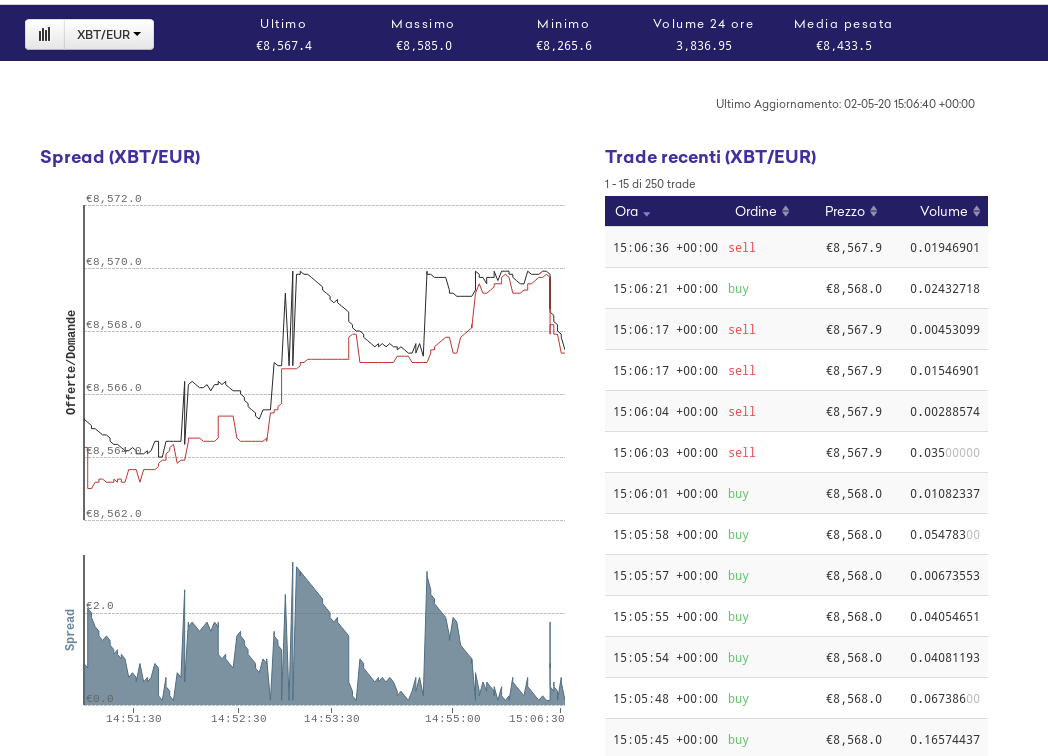
\includegraphics[width=10cm]{kraken_raw}
\end{center}
		\caption{\\~\\Figura: Elenco transazioni Bitcoin/Euro relative ad una finestra di minuti. I record mostrano l'ora in cui è avvenuto il trade, il tipo di operazione (buy / sell), il prezzo di scambio del titolo e la quantità di titoli scambiati. L'elenco dei dati di trade 'raw' è disponibile tramite le API kraken ed è la fonte grezza di dati finanziari utilizzati per calcolare i grafici OHLCV, fondamentali per l'analisi dei mercati. (fonte: https://www.kraken.com/)}
\end{fig}
\begin{fig}
\begin{center}
		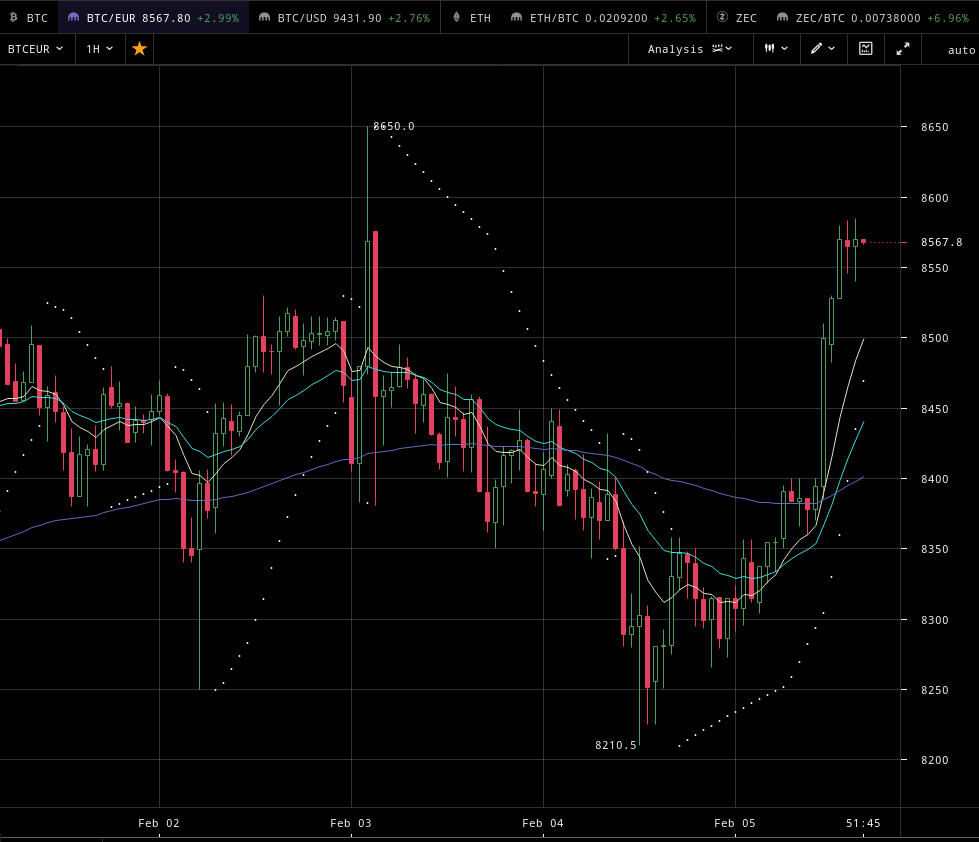
\includegraphics[width=\linewidth]{kraken_ohlcv}
\end{center}
		\caption{\\~\\Figura: Grafico OHLCV ricavato dai prezzi in Figura 1. Sulle ascisse è rappresentata l'ora mentre le ordinate sono il prezzo (in Euro) del titolo Bitcoin. Le "barre" orizzontali verdi e rosse sono le candele OHLCV: verdi se il prezzo è in crescita (\textit{open} minore di \textit{close}), rosse se in discesa (\textit{open} maggiore di \textit{close}). Le candele sono di durata 1 ora e, quindi i prezzi elencati nella precedente immagine rientrano soltanto in parte nell'ultima candela (rossa) delle 15:00 - 16:00, ancora aperta e, quindi, in creazione. La candela è rossa perchè, come si nota dai prezzi, il valore del titolo  è in discesa: partendo da circa 8.568 (probabilmente più alto nei record precedenti) si scende verso 8.567.\\
			Le linee colorate rappresentano le medie mobili dei prezzi di chiusura; usate per analisi tecnica, sono, rispettivamente, le medie a 10 (verde), 21 (azzurro) e 100 (blu) candele. Più candele sono considerate nella media e meno questa cambierà bruscamente, avendo, quindi, la media a 100 candele (cioè 100 ore) molto più lenta delle altre. (fonte: https://www.kraken.com/)}
\end{fig}

\\~\\Le immagini descrivono l'andamento dei prezzi scambio per scambio e le corrispondenti candele OHLCV come esposte dalla piattaforma di trading. I bordi orizzontali, che compongono i lati superiore ed inferiore della candela, sono il prezzo di apertura e quello di chiusura: se la candela è rossa, il prezzo di chiusura è minore di quello di apertura (significa che il prezzo dell'asset è sceso durante l'unità di tempo) e, quindi, il bordo superiore rappresenta il valore di \textit{open} e quello inferiore \textit{close}, mentre una candela verde indica una crescita del prezzo (\textit{open} è il lato inferiore mentre \textit{close} quello superiore). Le linee verticali della candela si estendono, invece, verso il prezzo minimo e massimo che l'asset ha toccato nel periodo di tempo fra apertura e chiusura della candela.
\\~\\
Le API di Kraken permettono di effettuare diversi tipi di operazioni, come:
\begin{itemize}
	\item scaricare lo storico dei prezzi di tutte le coppie valuta-criptovaluta disponibili dal 2013
	\item restare in attesa per ricevere in tempo reale i nuovi dati sugli scambi di titoli
	\item creare il proprio portafogli sulla piattaforma e piazzare ordini di acquisto e vendita
\end{itemize}
Tutte funzionalità ben sfruttate da Sentyment, che opera sul mercato in autonomia.



\section{Gudagnare con il trading}
E' importante notare che la ricchezza in possesso, calcolata in ogni istante, è data dalla quantità di budget e dalla quantità di titoli posseduti. Gli asset finanziari hanno un valore monetario indicato dal loro prezzo quindi, il possesso di alcuni di questi, anche se il budget da investire è azzerato, comporta, comunque, una ricchezza investita che si può recuperare rivendendo il titolo.\\
Si prende come esempio l'asset XBT/EUR, valuta di scambio fra Bitcoin e Euro. Partendo da un budget iniziale in Euro, bisogna decidere quando comprare titoli di Bitcoin e quando rivenderli per avere di nuovo Euro. Lo scopo della AI, quindi, non è soltanto massimizzare gli Euro in possesso, ma anche il numero di titoli Bitcoin, o del quantitativo di entrambi i titoli da avere in portafoglio, che porti all'aumento del loro valore.\\
A seconda delle aspettative sul rialzo o ribasso di un titolo è possibile agire in due modi: andare \textit{long} o andare \textit{short}. Andare \textit{long} vuol dire acquistare Bitcoin vendendo Euro, puntando ad un apprezzamento (aumento di valore) della criptovaluta; in questo caso, l’aspettativa è di un aumento del valore del cambio e si avrà, quindi, una visione rialzista (bullish) del mercato. Andare \textit{short} vuol dire vendere Bitcoin acquistando Euro, puntando, quindi, un apprezzamento dell'Euro nei confronti della criptomoneta. In questo caso, l’aspettativa è di una diminuzione di valore del cambio. Si aprirà, quindi, una posizione che mira ad una flessione del prezzo. La visione che il trader avrà del mercato sarà ribassista (bearish).\\~\\
Il punto centrale su cui si basano le strategie di investimento è indovinare se la valuta aumenterà o diminuirà di prezzo, per poi andare long o short a seconda della previsione. L'\textit{analisi tecnica} è un metodo riconosciuto e largamente utilizzato per anticipare, o prevedere, l'andamento dei prezzi e si basa sull'aspetto tecnico del mercato, utilizzando grafici e dati storici. In particolare, vengono analizzati prezzi, volumi scambiati e fasce temporali. Si utilizzano indicatori matematici, statistici e grafici. I segnali ed i suggerimenti ricavati da questi strumenti accompagnano i trader nelle loro decisioni in merito all'apertura e chiusura di posizioni di trading. L'analisi tecnica è un metodo di previsione dei prezzi basato sui dati storici.
\\~\\
%		\textbf{Altro su analisi tecnica?
%		https://www.xtb.com/it/scuola-di-trading/che-cosa-e-lanalisi-tecnica}
Supponendo che il mercato ad un certo punto cresca e si abbia "indovinato" un buon numero di previsioni, ci si ritroverà a possedere dei titoli che ora valgono un prezzo superiore rispetto al loro valore iniziale. Se i titoli crescono di valore, è bene, quindi, acquistarne finchè salgono, in questo modo si possiede un maggior numero di asset che andranno a valere sempre di più; in caso di perdita di valore del titolo, invece, generalmente, si dovrebbe vendere i titoli, per riacquistare del budget investito che ora stava perdendo valore e poterlo investire in altri titoli che crescono.\\
Quando si decide di acquistare, si sta effettuando la seguente operazione: dato un certo budget iniziale \textit{budget}, il valore del titolo \textit{price}, e la quantità di titolo acquistato \textit{equity} (Formula (1)) e supponendo di spendere sempre tutto il budget per acquistare il titolo
\\

\begin{equation}
equity=budget/price
\end{equation}
\\~\\
Mentre, all'occorrenza di un'operazione di vendita, utilizzando equity appena acquistata (Formula (2)):\\

\begin{equation}
budget=equity*price
\end{equation}

\\~\\
È possibile, in ogni momento, calcolare il ricavo o quantità di beni in possesso combinando il budget con equity, tenendo presente che, dopo un acquisto, il budget scende a zero e equity assume il valore indicato mentre, dopo una vendita, è equity a scendere a zero e si ritorna in possesso di budget. Lo stesso budget riacquistato verrà usato nuovamente per comprare dei titoli, facendo così crescere di nuovo equity, e così via. Un vincolo è quello di non poter effettuare due medesime operazioni di fila. 
\\~\\ 
Se si considera un certo budget iniziale \textit{initial\_budget}, il \textbf{guadagno} (\textit{gain}) in ogni istante è dato da:
\\
\begin{equation}
gain=(budget+equity*price)-initial\_budget
\end{equation}

\\~\\
Questa formula viene riutilizzata nel Capitolo 3 nell'ambito dello sviluppo degli strumenti di test.\\~\\
A questo punto, è necessario introdurre il concetto di \textit{fee}.\\
Le varie piattaforme di trading addebitano un costo per ogni singola operazione, di acquisto e di vendita, intestandosi una percentuale di budget speso dai trader come tassa per mantenere la piattaforma stessa.\\ Nel caso di operazioni di acquisto, la tassa è calcolata come percentuale del budget speso per comprare il titolo, quindi, viene scalata subito ed il risultato è l'acquisto di una quantità leggermente minore di titoli (la restante dei quali viene pagata alla piattaforma). Per le vendite, invece, la fee è tolta dal budget una volta che questo è ricalcolato vendendo equity, risultando in un ricavo leggermente minore di quello che si sarebbe ottenuto vendendo realmente l'intera quantità di titoli.\\
Nel caso di Kraken, la piattaforma di trading di riferimento su cui opera Sentyment, le fee sono del 0.26\%: significa che viene sottratto lo 0.26\% di budget che si intende investire, per ogni operazione. Per altri mercati, valute o piattaforme di trading, le fee possono variare e potrebbero non essere basate su una percentuale di acquisto, ma fisse (flat fee vs per share fee). Kraken applica una fee sempre fissa.
\\~\\
La presenza delle fee modifica abbastanza drasticamente il funzionamento del mercato e l'efficacia delle strategie di investimento, che devono essere adattate ad un mercato con fee; è necessario, quindi riscrivere le formule per il guadagno e per le operazioni di acquisto e vendita titoli, che ora comprendono la percentuale di fee.\\
Per gli acquisti, considerando un certo budget iniziale \textit{budget} (o il budget risultato di una precedente vendita), il valore del titolo \textit{price}, la quantità di titolo acquistato \textit{equity} e una tassa \textit{fee}:\\
\begin{equation}
equity=(budget*(1-fee))/price
\end{equation}
\\~\\
Per le vendite:\\
\begin{equation}
budget=(equity*price)*(1-fee)
\end{equation}
\\~\\ Dal momento che le budget e equity sono già calcolati, togliendo le fee per ogni operazione di acquisto e vendita, la formula del guadagno rimane la stessa.\\~\\
%		\textbf{ESEMPIO DI COME CAMBIEREBBE RISULTATO CON E SENZA FEE CON POCHI DATI DI ESEMPIO?}
Senza addentrarsi nelle diversità dei titoli e dei mercati, si può affermare che una strategia generale, e semplificata, per guadagnare facendo trading è \textit{compra basso, vendi alto}; nella realtà i segnali di acquisto possono essere dati da altri indicatori più complessi e non sempre è possibile capire quando un titolo sta toccando un prezzo particolarmente alto o basso: è facile analizzare i grafici a posteriori, ma non altrettanto semplice prevedere massimi e minimi locali online. Per questo, si utilizzano delle semplici strategie fondamentali che aiutano a capire l'andamento dei prezzi.


\section{Esempi di strategie}
Come già accennato, l'\textit{analisi tecnica} è lo studio dell'andamento dei prezzi dei mercati finanziari nel tempo, allo scopo di prevederne le tendenze future, mediante, principalmente, metodi grafici e statistici. In senso lato, è quella teoria di analisi secondo cui è possibile prevedere l'andamento futuro del prezzo di un bene quotato, studiando la sua storia passata. Viene utilizzata, assieme all'\textit{analisi fondamentale}, per la definizione delle decisioni di operatività finanziaria.\\ Volendo distinguere l'analisi fondamentale da quella tecnica, si può dire che, mentre l'analisi tecnica cerca di definire il prezzo futuro di un titolo, basandosi sugli aspetti formali dell'andamento delle quotazioni (derivati da grafici), l'analisi fondamentale si occupa di stabilire il prezzo corretto di un titolo in base alle caratteristiche economico-finanziarie intrinseche della società cui fa riferimento.\\~\\L'analisi tecnica si prefigge di analizzare, e comprendere, attraverso l'analisi del grafico, l'andamento dei prezzi il quale, a sua volta, rispecchia le decisioni degli investitori;  si basa, inoltre, sull'assunto fondamentale che, poiché il comportamento degli investitori si ripete nel tempo, al verificarsi di certe condizioni grafiche, anche i prezzi si muoveranno di conseguenza. Il compito principale dell'analisi tecnica è, quindi, quello di identificare un cambiamento di tendenza rispetto ad uno stadio iniziale, mantenendo una posizione di investimento fino a quando non vi sia prova che la tendenza stessa si sia di nuovo invertita.\\
Per individuare un trend si fa uso di indicatori tecnici, basati su prezzo e volume, calcolati a partire dai grafici: questi analizzano i movimenti di prezzo a breve termine e alcuni dei più noti ed usati sono Moving Average Crossover, MACD (moving average convergence / divergence), RSI (relative strength index) e Bollinger Bands.\\
Analizzando i grafici passati mediante queste strategie, è possibile ricavare i parametri per gli indicatori che meglio si adattano al mercato in analisi e riutilizzare l'indicatore, applicandolo ai dati futuri, per identificare nuovi trend.\\~\\

\subsection{Moving Average Crossover}
Questa strategia prevede il calcolo di una o più medie mobili a diverso periodo, le cui intersezioni nel grafico definiscono un segnale di buy o sell.\\
Il moving average \textit{crossover} si verifica quando, nel grafico di due medie mobili, ciascuna basata su diversi periodi, le linee di queste medie mobili si incrociano.\\ Non prevede la direzione futura ma mostra le tendenze. Questo indicatore utilizza due (o più) medie mobili, una più lenta ed una più veloce. La più veloce è una media mobile a breve termine. Per i mercati azionari di fine giornata, ad esempio, può essere un periodo di 5, 10 o 25 giorni, mentre, la più lenta è la media mobile di medio o lungo termine (ad esempio periodo di 50, 100 o 200 giorni). Una media a breve termine è più veloce perché considera i prezzi solo per un breve periodo di tempo ed è, quindi, più reattiva alle variazioni giornaliere dei prezzi. D'altra parte, una media mobile a lungo termine è considerata più lenta in quanto incapsula i prezzi per un periodo più lungo; tende, tuttavia, ad attenuare i disturbi che si riflettono spesso nelle medie mobili a breve termine.
\\
Una moving average, come una linea a sé stante, viene spesso sovrapposta nei grafici per indicare l'andamento dei prezzi. Un crossover si verifica quando una media mobile più veloce (cioè una media mobile di periodo più breve) attraversa una media mobile più lenta (cioè una media mobile di periodo più lungo).\\
In altre parole, accade quando la linea della media mobile del periodo più breve attraversa una linea della media mobile del periodo più lungo: questo punto di incontro viene utilizzato per comprare o vendere titoli. Quando la media veloce supera quella lenta, si ha un segnale di \textit{buy}, mentre \textit{sell} se viceversa.\\~\\
\begin{fig}
	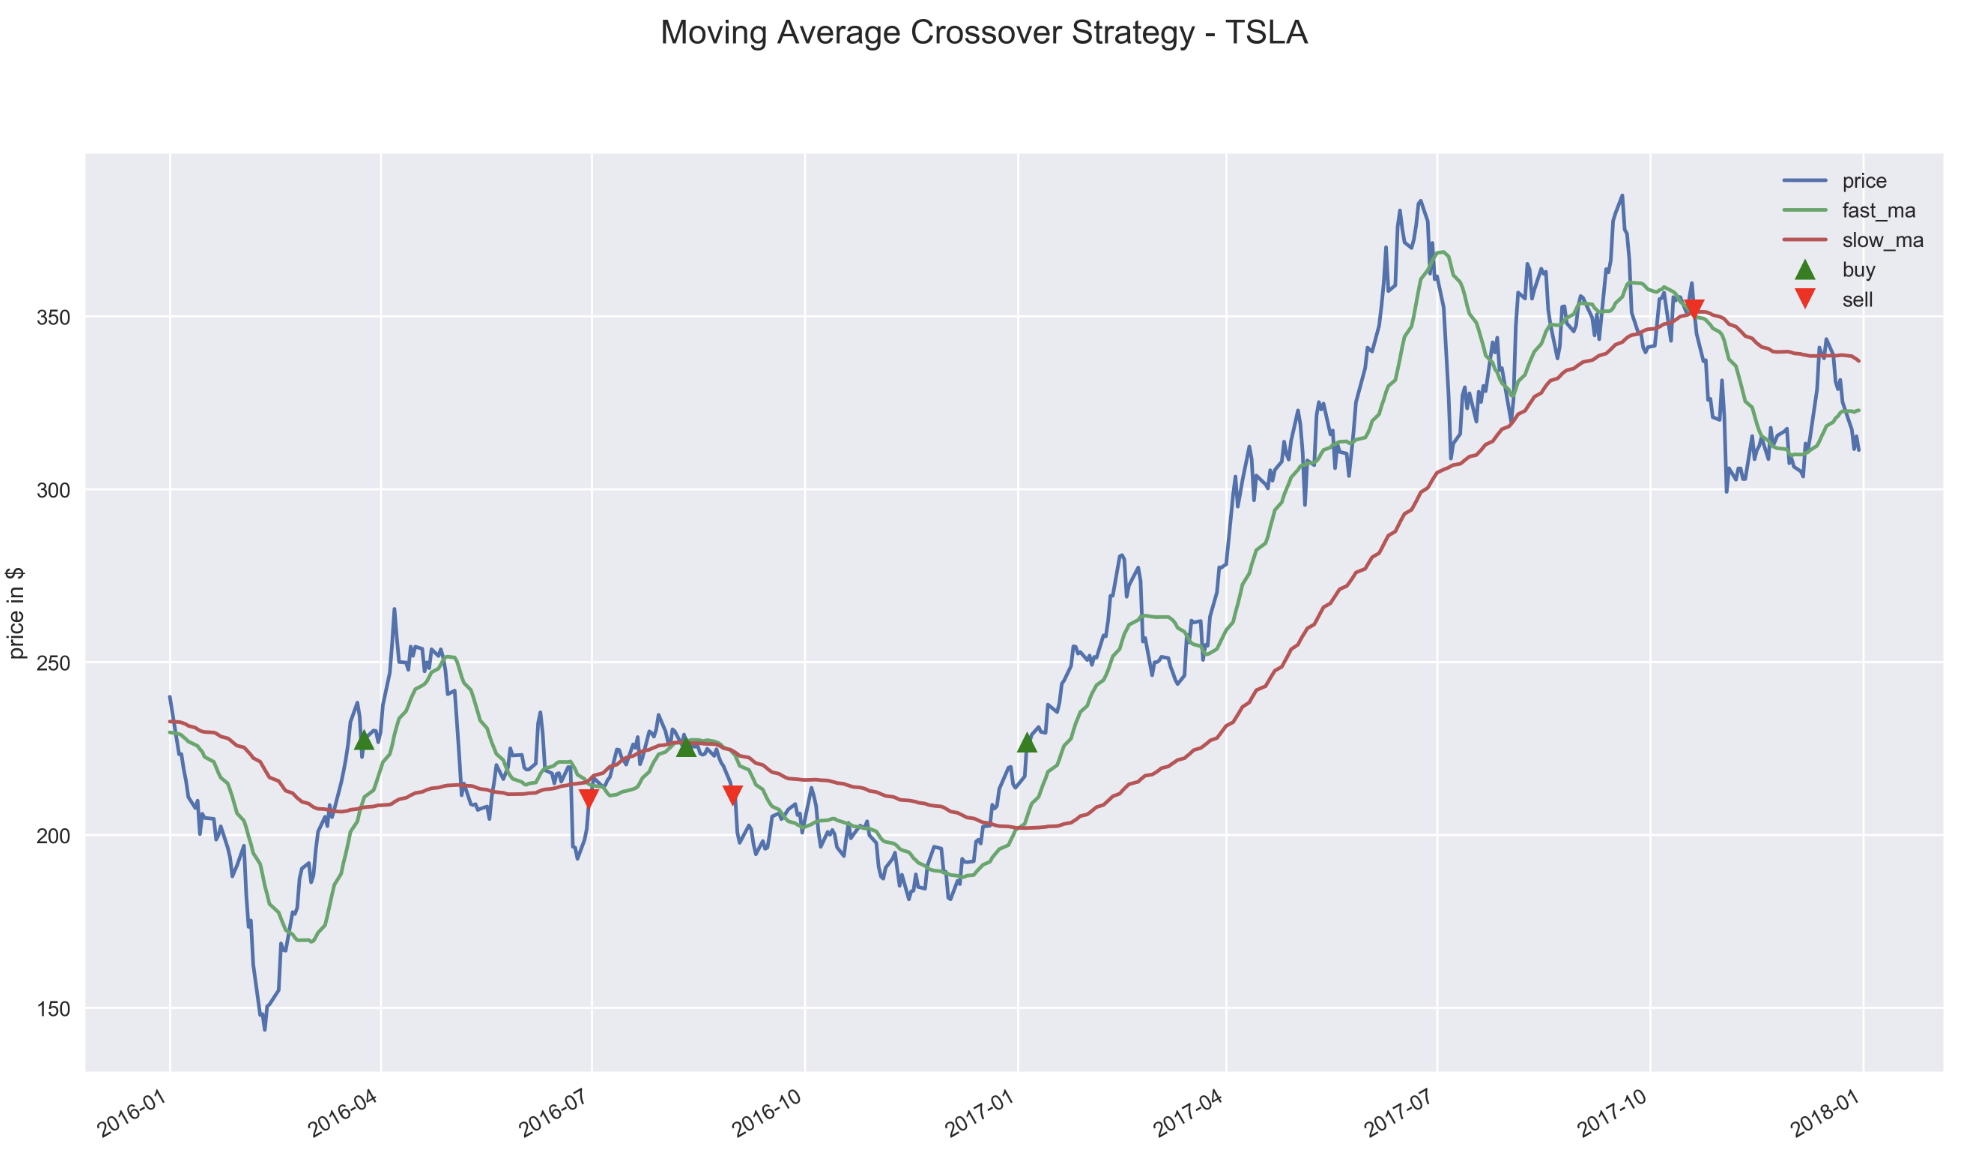
\includegraphics[width=\linewidth]{moving_avg}
	\caption{Figura: Andamento dei prezzi per il titolo TESLA/DOLLARO, accompagnato da due medie mobili a diverso periodo: fast\_ma a 20 giorni mentre slow\_ma a 100 giorni. Le frecce verdi e rosse indicano i segnali di buy e sell ricavati dalle intersezioni fra le medie.}
\end{fig}
\\~\\Esistono diverse declinazioni della strategia a medie mobili, come ad esempio SMA (simple moving average), che utilizza come segnale di buy / sell il crossover fra i prezzi di chiusura e la media mobile semplice; EMA usa una media esponenziale; MACD (moving average convergence / divergence) usa come prima statistica la differenza fra la media veloce e quella lenta e, come seconda statistica, la media di queste differenze.
%		\\\textbf{PARLARE DI TUTTE LE STRATEGIE? MACD, RSI, BOLLINGER?}
\\~\\
Calcolati gli indicatori statistici più adatti alla situazione, e scelti i parametri migliori (come i periodi delle medie da usare), si è costruito un modello di trend del titolo e si è in grado di prevedere quando il trend si ripropone. Prendendo l'esempio di una moving average crossover con una media veloce e una lenta, analizzato che per la maggior parte dei casi si riscontra un guadagno vendendo quando la media lenta supera quella veloce, e comprando quando accade l'opposto, allora, si può affermare che sarà molto probabile guadagnare ancora, in futuro, ripetendo le medesime operazioni.

\subsection{Buy-Hold}
Un altro esempio di strategia, molto più semplice di Moving Average Crossover e, in questo ambito, utilizzata più come base per confrontare l'efficacia di altre strategie, che come tecnica vera e propria per massimizzare i guadagni .\\
Buy and hold, comprare e detenere, chiamato anche trading di posizione, è una strategia di investimento in cui un investitore acquista titoli e li detiene a lungo, con l'obiettivo che i titoli aumentino gradualmente di valore per un lungo periodo di tempo. Ciò si basa sull'idea che, a lungo termine, i mercati finanziari offrano un buon tasso di rendimento, pur tenendo conto di un certo grado di volatilità. Questo punto di vista sostiene che la tempistica del mercato, ovvero il concetto che si può entrare nel mercato ai minimi e vendere ai massimi, non funziona; tentare tale tempismo dà risultati negativi, almeno per gli investitori piccoli o poco sofisticati quindi, è meglio per loro semplicemente acquistare e detenere.\\~\\ I segnali di buy e sell si riducono, quindi, semplicemente, a uno solo: comprare all'inizio del periodo considerato (appena si vuole utilizzare la strategia) e non vendere \textit{mai}. Supponendo che il valore del titolo continui sempre a crescere, sul lungo periodo, si avrà un aumento delle \textit{equity} acquistate e, quindi, un aumento della ricchezza posseduta. Infatti, facendo riferimento alla formula del guadagno (Formula (3)), se \textit{equity} sale e \textit{budget} rimane sempre a 0, il guadagno sale, essendo direttamente proporzionale al prezzo del titolo posseduto. La strategia, pertanto, segue l'andamento del mercato: se il valore del titolo sale, il guadagno associato sale mentre, in corrispondenza di un calo, anche la ricchezza posseduta nell'investimento scende.\\
Un vantaggio introdotto da questa strategia è la quasi totale assenza di costi dovuti alle fee. Effettuando una sola operazione di buy iniziale, in cui la fee viene pagata, non è più necessario vendere o comprare ulteriormente e, quindi, sempre nell'ottica di un aumento di valore del titolo a lungo termine, il guadagno aumenta senza dover spendere ulteriore capitale in fee associate ad altre operazioni.\\~\\

\begin{fig}
	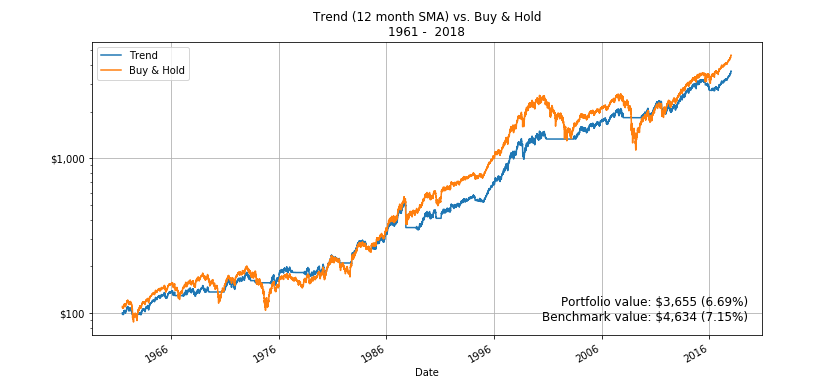
\includegraphics[width=16cm]{buy_hold}
	\caption \\~\\Figura: esempio dell'andamento di prezzi del titolo S\&P 500, rappresentato con una media mobile a 12 mesi, e valore della ricchezza prodotto da una strategia buy-hold. La media ammortizza la variazione di prezzo e rimane più costante, mentre buy-hold si vede assumere tutti i valori di prezzo del titolo. Come si può notare, buy-hold segue esattamente l'andamento del mercato: il valore del portafoglio (guadagno, Formula 3) dipende dal valore del titolo. Analizzando i prezzi dal 1966 al 2016 si nota una lenta salita e quindi buy-hold si rivela comunque efficace.
\end{fig}
\\~\\La strategia è tuttavia utilizzata quasi esclusivamente come \textit{benchmark}, metodo di confronto per le vere strategie che si applicano nel contesto di trading, o si sviluppano ed implementano nei vari algoritmi di AI per trading. Il minimo che un algoritmo, o nuova strategia, possa fare è quello di \textit{battere buy-hold}. Il metodo di confronto di due strategie è trattato nel Capitolo 4 ma, semplificando molto, si può affermare che, dal punto di vista esclusivamente del guadagno totale, considerando due strategie che partono e terminano entrambe nello stesso momento, una è migliore dell'altra se porta ad un guadagno finale maggiore. Nella realtà sono usati diversi indicatori aggiuntivi, oltre al guadagno, e va definito quale ha maggiore importanza per i fini dell'investitore. Una strategia potrebbe rivelarsi migliore di altre se si considera il guadagno, mentre potrebbe risultare la peggiore se la metrica usata è, per esempio, il rischio di perdita.\\~\\Ad ogni modo, qualsiasi sia il metro di paragone per il confronto delle strategie, buy-hold è la più semplice che si possa concepire e, se si volesse creare una nuova strategia, questa deve fornire risultati migliori comparata a buy-hold, altrimenti non può considerarsi molto efficace.


\section{Ruolo delle intelligenze artificiali e scopo della tesi}		
L'apprendimento automatico, e diverse tecniche hanno creato nuovi sistemi per individuare pattern, cosa che il cervello umano non è in grado di fare. Dal momento che la finanza è quantitativa, la AI, nel trading azionario, sta guadagnando terreno. Le società finanziarie hanno investito molto nell'intelligenza artificiale in passato e studiano ed implementano le applicazioni finanziarie di machine learning e del deep learning nelle loro operazioni.\\
L'analisi tecnica è, dunque, implementata in sistemi automatici, che sono molto più efficienti di un trader umano ed offrono diversi vantaggi. Le AI separano le informazioni prevedibili da qualsiasi "rumore casuale", gli algoritmi apprendono dall'accuratezza delle previsioni precedenti e si adeguano continuamente, abbastanza veloci da prevedere il mutamento della situazione del mercato, anche in un orizzonte di pochi giorni. Possono imparare dai successi e fallimenti e riconfigurare, ogni giorno, le approssimazioni del funzionamento interno del mercato, poiché viene alimentato con nuovi dati.\\
Oltre agli indiscutibili vantaggi computazionali di una macchina rispetto al cervello, ci sono altri aspetti da considerare che hanno portato alla crescita delle AI nel settore. Si può infondere la conoscenza degli esperti dell'ambito in un software che si auto adatta e migliora, senza avere gli svantaggi dell'errore umano; si può estendere per permettergli di gestire diversi ambiti, dal recupero della materia prima (i dati di trading) fino alla vendita del prodotto finito (vendita di strategie di investimento). È possibile costruire sistemi complessi che modellano intere realtà.\\~\\
Sentyment è uno di questi software descritti. Si occupa di raccogliere dati, elaborarli e, attraverso una AI, li analizza per produrre strategie di investimento. Il modulo di intelligenza artificiale è molto ampio: esistono molte AI che operano producendo costantemente nuovi segnali di buy / sell per le strategie e sono monitorate da una ulteriore, singola AI. Questo supervisore, \textit{meta-learner}, decide quale, fra le molte AI, sta avendo più successo e la promuove come attiva da utilizzare.\\
Lo scopo della tesi è sviluppare il supervisore ed inserirlo all'interno del complesso sistema di Sentyment, impiegando tecniche di test per intelligenze artificiali che permettano di scegliere un rappresentante migliore fra una serie di agenti che operano indipendentemente.
\\~\\
\begin{fig}
	\begin{center}
		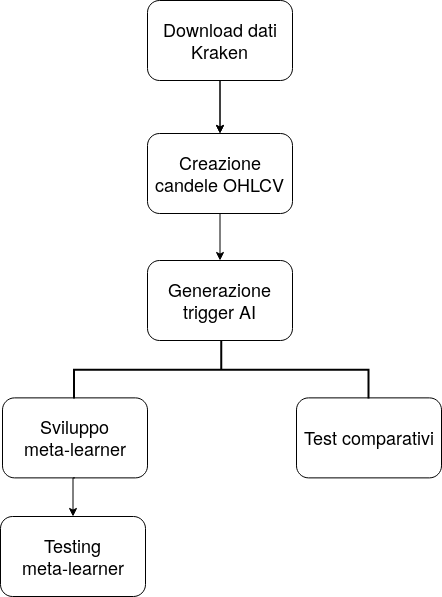
\includegraphics[width=10cm]{flowchart}
	\end{center}
	\caption{\\~\\Figura: Diagramma delle attività svolte, spiegate nel dettaglio in ogni relativo capitolo. La fase preliminare di download dati comporta la successiva analisi esplorativa degli stessi e fornisce l'input per il resto del sistema. Il passo successivo è la creazione di candele OHLCV, cioè il tipo di dato utilizzato dalle AI. A questo punto la AI Sentyment può mettere in moto i suoi algoritmi per produrre le strategie di investimento, ovvero l'elenco di operazioni buy / sell (\textit{trigger}) per ogni istante di tempo. Da qui si sono svolte due differenti attività: l'analisi dei risultati prodotti dalla AI (test comparativi) e lo sviluppo della AI supervisore (\textit{meta-learner}), con successiva analisi e testing dei suoi risultati.}
\end{fig}



\newpage
\chapter{AI per financial prediction e Sentyment}
\label{cap2}
La predizione del mercato azionario è stata una questione importante nel campo della finanza, ingegneria e matematica, a causa del suo potenziale guadagno finanziario. Data la grande quantità di capitale negoziato attraverso il mercato azionario, questo è visto come una grande opportunità ed ha richiamato molti investimenti. La previsione del mercato azionario, inoltre, comporta la sfida di dimostrare se il mercato finanziario sia prevedibile oppure no. Dal momento che non c'è stato consenso sulla validità dell'ipotesi che nel mercato ci sia spazio per la predizione, i ricercatori hanno molto faticato per dimostrarne la prevedibilità\cite{nn1}. L'\textit{ipotesi del mercato efficiente} (EMH: Efficient Market Hypotesis) è un'ipotesi in economia finanziaria che afferma che i prezzi delle attività riflettono tutte le informazioni disponibili. Una conseguenza diretta è che è impossibile "battere il mercato" in modo coerente basandosi sul rischio poiché i prezzi di mercato dovrebbero reagire solo a nuove informazioni. È una teoria che fa sorgere molte controversie e, come tale, non ancora dimostrata, il che lascia spazio ai tentativi di sviluppo di un algoritmo che sia in grado di prevedere parte dell'andamento dei mercati.\\~\\
Con l'avvento di computer più veloci, e vaste informazioni su Internet, i mercati azionari sono diventati più accessibili agli investitori strategici o al pubblico generale. Internet fornisce la fonte principale di informazioni ed ha un impatto significativo sui mercati azionari, e le tecniche di estrazione ed utilizzo delle informazioni a supporto del processo decisionale hanno raggiunto un'importanza critica. Per prevedere il mercato azionario con precisione, vari algoritmi e modelli di predizione sono stati proposti da molti ricercatori, sia accademici che nell'industria.\\~\\

\section{Stato dell'arte delle AI}
Da quando il mercato azionario è stato introdotto per la prima volta, molti hanno tentato di prevederne il comportamento utilizzando vari strumenti computazionali come \textit{Linear egression} (LR), \textit{Neural Network} (NNs), \textit{Genetic Algorithm} (GA), \textit{Support Vector Machine} (SVMs), \textit{Case-based Reasoning} (CR) e altri.\\~\\
Nell'ultimo decennio, Neural Network sono state ampiamente utilizzate, ed in molti casi hanno mostrato prestazioni migliori rispetto ad altri approcci. Una \textbf{rete neurale} (NN "Neural Network"), è un modello matematico/informatico di calcolo basato sulle reti neurali biologiche. Tale modello è costituito da un gruppo di interconnessioni di informazioni costituite da neuroni artificiali e processi che utilizzano un approccio di connessionismo di calcolo. Nella maggior parte dei casi, una rete neurale artificiale è un sistema adattivo che cambia la propria struttura in base ad informazioni esterne, od interne, che scorrono attraverso la rete stessa durante la fase di apprendimento.\\~\\
Il primo modello di previsione del mercato azionario basato su Neural Network è stato implementato da White\cite{whitenn}. Ha usato \textit{Feed Forward Neural Networks} (FFNN)\footnote{Una rete neurale feed-forward ("rete neurale con flusso in avanti") o rete feed-forward è una rete neurale artificiale dove le connessioni tra le unità non formano cicli, differenziandosi dalle reti neurali ricorrenti. In questa rete neurale le informazioni si muovono solo in una direzione, avanti, rispetto a nodi d'ingresso, attraverso nodi nascosti (se esistenti) fino ai nodi d'uscita. Nella rete non ci sono cicli. Le reti feed-forward non hanno memoria di input avvenuti a tempi precedenti, per cui l'output è determinato solamente dall'attuale input. } per decodificare regolarità precedentemente non rilevate nei movimenti di prezzo degli asset, come fluttuazioni di prezzo di azioni ordinarie, ed ha mostrato come cercare tali regolarità usando FFNNs. Dal tentativo iniziale di White, un numero di ricercatori ha partecipato allo sviluppo di un modello di previsione del mercato azionario accurato. Phua et al. \cite{puann} ha utilizzato Neural Network con Genetic Algorithm per prevedere l'indice di scambio del mercato azionario di Singapore\footnote{L'indice FTSE Straits Times (STI) è un indice di borsa ponderato per la capitalizzazione che è considerato l'indice di riferimento per il mercato azionario di Singapore. Tiene traccia delle prestazioni delle prime 30 società quotate alla Borsa di Singapore.}, ottenendo un tasso di accuratezza dell'81\%. Kim e Han \cite{kimnn} hanno anche combinato Neural Network con Genetic Algorithm e pronosticato Korea Composite Stock Index 200\footnote{Korea Composite Stock Index (KOSPI): indice di borsa azionario della Corea del Sud, che ospita più di 780 società quali Samsung, Hyundai e Kia motors}. He raggiunto l'82\% di accuratezza nel prevedere sia le tendenze in aumento ed in calo del mercato azionario.\\~\\
Genetic Algorithm è stato studiato e dimostrato essere efficace nell'esplorare uno spazio complesso in modo adattivo, guidato dal meccanismo evolutivo di riproduzione, crossover e mutazione.\\
Un \textbf{algoritmo genetico} è un algoritmo euristico\footnote{Un algoritmo euristico, o \textit{euristica}, è un particolare tipo di algoritmo progettato per risolvere un problema più velocemente, nel caso in cui i metodi classici siano troppo lenti nel calcolo (ad esempio, in caso di elevata complessità computazionale) o per trovare una soluzione approssimata, nel caso in cui i metodi classici falliscano nel trovare una soluzione esatta.} utilizzato per tentare di risolvere problemi di ottimizzazione per i quali non si conoscono altri algoritmi efficienti di complessità lineare o polinomiale. L'aggettivo "genetico", ispirato al principio della selezione naturale ed evoluzione biologica, deriva dal fatto che gli algoritmi genetici attuano dei meccanismi concettualmente simili a quelli dei processi biochimici scoperti dalla biologia.\\
In sintesi, gli algoritmi genetici consistono in algoritmi che permettono di valutare diverse soluzioni di partenza (come se fossero diversi individui biologici) e che, ricombinandole  ed introducendo elementi di disordine (mutazioni genetiche casuali), producono nuove soluzioni che vengono valutate scegliendo le migliori nel tentativo di convergere verso soluzioni "di ottimo". Nonostante questo utilizzo nell'ambito dell'ottimizzazione, data la natura intrinsecamente casuale dell'algoritmo genetico, non vi è modo di sapere, a priori, se sarà effettivamente in grado di trovare una soluzione accettabile al problema considerato. La soluzione trovata sarà frutto di una procedura casuale e, quindi, difficilmente riproducibile. 
\\~\\
Di recente, molti ricercatori hanno impiegato Genetic Algorithm per migliorare le prestazioni delle tecniche di AI. Nell'ambito delle Neural Network, Genetic Algorithm  è comunemente usato per selezionare la topologia di rete e determinare il numero ottimale di layer nascosti e di elementi di elaborazione.\\~\\
Molti ricercatori hanno confrontato le Neural Network con approcci statistici per il riconoscimento di pattern \cite{nng}\cite{nns}. Yoon et al. \cite{nny} ha sottolineato la superiorità di Neural Network sull'analisi discriminante classica. Garliauskas \cite{nng} ha, inoltre, esaminato la previsione del mercato azionario utilizzando Neural Network in combinazione con un approccio alle \textit{funzioni kernel}\footnote{Le funzioni kernel sono una classe di algoritmi per l'analisi di pattern, schemi, il cui elemento maggiormente conosciuto sono le Support Vector Machine (SVM). Lo scopo generale dell'analisi di pattern è di trovare, e studiare, tipi generici di relazioni. Le funzioni kernel si approcciano al problema mappando i dati in uno spazio di caratteristiche multidimensionale, trasformando i dati in un insieme di punti dello spazio euclideo.} ed il metodo dell'errore di previsione ricorsivo\footnote{Errore di predizione: è una misura di quanto bene il modello prevede la variabile di risposta, o di come i campioni sono classificati nella categoria corretta.}.\\
Garliauskas \cite{nng} ha concluso che, nel prevedere le serie temporali finanziarie, le Neural Network hanno prestazioni migliori rispetto ai metodi statistici classici. In generale, numerosi studi hanno dimostrato che le Neural Network hanno la capacità di prevedere i mercati azionari in modo più accurato rispetto ad altri metodi \cite{nny}\cite{nnk}\cite{nnp}\cite{nns2}.

\subsection{Supporto di informazioni relative agli eventi}
Sebbene gli studi precedenti fossero limitati ad analisi quantitativa, diversi studi recenti sono stati eseguiti sulla base dell'analisi qualitativa. Molti credevano che l'integrazione di una conoscenza degli eventi nelle Neural Network risultasse promettente per una migliore previsione del mercato azionario \cite{know-nn}\cite{news-nn}\cite{know-nn2}\cite{news-nn2}. Kohara \cite{know-nn2} ha studiato alcune metodologie per migliorare i modelli predittivi multivariati\footnote{Il modello multivariato è un comune strumento statistico che utilizza più variabili per prevedere i possibili risultati. Gli analisti della ricerca utilizzano modelli multivariati per prevedere i risultati degli investimenti in diversi scenari, al fine di comprendere l'esposizione che un portafoglio ha a particolari rischi. Ciò consente, ai gestori di portafoglio, di mitigare meglio i rischi identificati attraverso l'analisi della modellazione multivariata. La \textbf{simulazione Monte Carlo} è un modello multivariato ampiamente utilizzato che crea una distribuzione di probabilità che aiuta a definire una gamma di possibili risultati di investimento.} nella previsione del prezzo delle azioni utilizzando Neural Network e conoscenza pregressa. Ha usato le informazioni dai titoli dei giornali per migliorare la capacità di previsione. I loro risultati sperimentali hanno dimostrato che, l'utilizzo della conoscenza degli eventi unita alle Neural Network ha ridotto significativamente il tasso di errore di previsione intorno al livello di significatività del 5\% con profitto del 40\%.\\~\\
Inoltre, Hong e Han \cite{know-nn} hanno confrontato le Neural Network con informazioni sugli eventi rispetto al modello \textit{Random Walk} (RW)\footnote{In matematica, una passeggiata aleatoria (Random Walk) è la formalizzazione dell'idea di prendere passi successivi in direzioni casuali. Matematicamente parlando, è il processo stocastico più semplice.} e, rispetto a Neural Network, senza informazioni sull'evento. Neural Network con informazioni sull'evento hanno una media dello 0,527\% di errore, che è un errore minore rispetto ad altri modelli. Hanno dimostrato che le previsioni basate su Neural Network sono notevolmente superiori a Random Walk e che l'effetto dell'informazione sugli eventi esiste.\\
Nella previsione mercato azionario, inoltre, molti ricercatori hanno riconosciuto che fattori qualitativi, quali effetti politici ed eventi internazionali, hanno svolto un ruolo molto importante. Hanno, dunque, proposto che un sistema di previsione del mercato azionario debba incorporare fattori sia quantitativi che qualitativi. I loro studi hanno, infine, dimostrato che le Neural Network che si basano sui fattori sia quantitativi che qualitativi sono di gran lunga superiori a quelle basati solo su fattori quantitativi \cite{fuzzy-nn1}\cite{fuzzy-nn2}.

\subsection{Punti chiave nelle predizioni finanziarie}
Numerosi ricercatori hanno mostrato il loro ufficiale punto di vista sull'\textit{ipotesi del mercato efficiente} (EMH: efficient market Hypotesis) in ambito accademico \cite{emh1}\cite{emh2}. EMH afferma che l'attuale prezzo di mercato riflette l'assimilazione di tutte le informazioni disponibili\cite{emh3}. L'informazione rilevante per un mercato è contenuta nei prezzi e, ogni volta che sorgono nuove informazioni, il mercato corregge se stesso e le assorbe, quindi, il mercato è efficiente e non c'è spazio per la predizione\cite{emh4}.\\~\\
È in corso un lungo dibattito sulla validità di EMH, ma non è stato raggiunto un consenso. Negli ultimi anni, molti i ricercatori hanno affermato che, sicuramente, EMH deve essere falso\cite{emh4}. Diversi studi sono stati condotti sui dati dei mercati azionari al fine di dimostrare che il mercato è prevedibile. Se qualche sistema di calcolo avesse la capacità di mostrare previsioni con ragionevole accuratezza, basandosi sui dati storici di mercato, allora la validità di EMH potrebbe essere messa in discussione.\\
Tsibouris e Zeidenberg\cite{emh0} hanno utilizzato le Neural Network per prevedere il mercato azionario basandosi soltanto sui prezzi passati come input. I loro risultati empirici hanno mostrato un certo livello di capacità predittiva e respinto la forma debole di EMH\footnote{La forma debole dell'\textit{ipotesi di mercato efficiente} (EMH, efficient market hypotesis) afferma che i prezzi passati, i valori storici e le tendenze non possono prevedere i prezzi futuri. I prezzi delle azioni riflettono soltanto tutte le informazioni attuali}.\\
Eyden \cite{nn-eyden} ha sviluppato, inoltre, un sistema che modella le prestazioni della borsa azionaria di Johannesburg ed il loro sistema ha fornito prove significative dimostrando la sua capacità di prevedere le direzioni del mercato azionario, quindi, di nuovo, dissentendo da EMH.\\~\\
Dalla parte opposta, invece, vari studi sono basati sull'ipotesi di mercato efficiente. Fung et al. \cite{news-nn} ha indagato sull'immediato impatto delle notizie di giornale sulle serie storiche basate su EMH. Hanno presentato un sistema basato su EMH per prevedere il comportamento futuro del mercato azionario utilizzando informazioni non quantificabili (notizie dai giornali) e le previsioni sono state fatte solo in base al contenuto dell'articolo. Alla fine, il loro risultato empirico ha indicato che l'approccio basato su EMH è più redditizio rispetto alla semplice strategia di trading basata su Buy-Hold\footnote{Buy and Hold: strategia di investimento, usata spesso come base per confrontare altre strategie. Un investitore acquista titoli e li detiene a lungo, con l'obiettivo di aumentare gradualmente, col tempo, il loro valore. Il guadagno segue l'andamento del mercato: il valore del titolo può salire o scendere. È la strategia minimale da "battere" se si vogliono sviluppare nuove strategie: compra e detieni, senza fare niente.}. Come è stato discusso, diversi studi hanno concluso di accettare, o confutare, EMH. La questione dell'efficienza del mercato, dunque, non è ancora pienamente indagata e porta alla necessità di ulteriori ricerche.\\~\\
Un certo numero di ricercatori ha usato la cronologia dei dati numerici delle serie temporali per la previsione dei mercati azionari ed ha raggiunto una ragionevole accuratezza delle previsioni rifiutando l'ipotesi di EMH \cite{nn-eyden}\cite{emh0}.\\Tuttavia, ci sono vari fattori che influenzano i prezzi delle azioni, come le prestazioni e la robustezza di un'azienda, le tendenze del mercato, la psicologia degli investitori, il coinvolgimento del governo, i cambiamenti nell'attività economica e così via. Molti ricercatori, quindi, hanno concordato sull'esistenza di una correlazione significativa tra gli eventi che rappresentano i fattori sopra citati ed i mercati azionari \cite{news-nn}\cite{know-nn2}. Hanno utilizzato le informazioni relative agli eventi in aggiunta a quelle numeriche delle serie temporali e raggiunto un certo livello di precisione nelle previsioni. Poiché, però, ogni evento ha un diverso livello di impatto in termini di intervallo di tempo in cui l'evento stesso può influenzare il mercato, ogni evento dovrebbe essere ponderato in base al suo livello di impatto, che è definito sulla base della conoscenza preliminare costruita in precedenza. In aggiunta, il web è visto come la principale fonte di informazione sugli eventi per la previsione di mercato, contenendo le più aggiornate e preziose informazioni. Sono necessarie, pertanto, tecniche automatiche di \textit{web mining}\footnote{Il web mining è la raccolta sistematica di dati provenienti dal web, organizzati e visualizzati al fine di far emergere informazioni utili. Prevede l'impiego di tecniche di data mining al fine di estrapolare dati da server e pagine web.} per ottenere un livello più elevato di accuratezza della previsione in tempi brevi.

\subsection{Metodi di previsione}

\begin{fig}
	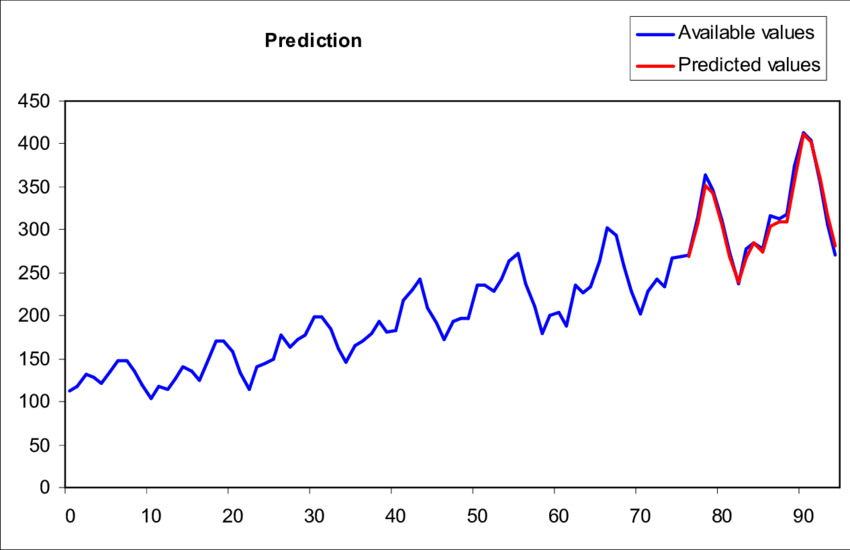
\includegraphics[width=15cm]{time_series}
	\caption{\\~\\Figura: esempio di utilizzo di una tecnica per predizione. Si suppone di analizzare il grafico dell'andamento di un titolo (serie storica), in cui le ascisse sono il tempo e le ordinate il prezzo dell'asset. Come si può notare, molto spesso, nelle serie storiche finanziarie, i pattern si ripetono nel tempo e, applicando metodi di regressione o intelligenza artificiale, è possibile prevedere quando questi si ripresenteranno.}
\end{fig}

\subsubsection{Predizione tradizionale di serie storiche}
I modelli statistici tradizionali sono ampiamente utilizzati in economia per la previsione di serie storiche\footnote{In statistica descrittiva, una serie storica o temporale ("time series") si definisce come un insieme di variabili casuali ordinate rispetto al tempo, ed esprime la dinamica di un certo fenomeno nel tempo. Le serie storiche vengono studiate sia per interpretare un fenomeno, individuando componenti di trend, di ciclicità, di stagionalità e/o di accidentalità, sia per prevedere il suo andamento futuro. }. Questi modelli sono in grado di modellare relazioni lineari tra fattori che influenzano il mercato ed il valore del mercato. In economia, ci sono due tipi di previsione delle serie: univariata (regressione semplice) e multivariata (regressione multivariata) \cite{emh2}. Un esempio ampiamente usato di modello univariato è Box-Jenkins\footnote{Il modello autoregressivo a media mobile, detto anche ARMA, è un tipo di modello matematico lineare che fornisce, istante per istante, un valore di uscita basandosi sui precedenti valori in entrata ed in uscita. A volte denominato modello di Box-Jenkins, dal nome dei suoi inventori, viene utilizzato, in statistica, per lo studio delle serie storiche dei dati.}, che contiene solo una variabile nell'equazione ricorrente. Mostra un processo complesso di adattamento dei dati ai parametri appropriati del modello. Nelle loro equazioni sono inclusi i valori passati delle medie mobili dei prezzi.\\~\\
Sebbene Box-Jenkins mostri una buona capacità di previsione a breve termine, richiede una grande quantità di dati per fornire un'alta precisione \cite{23}. I modelli multivariati sono modelli univariati ampliati per "scoprire i fattori causali che incidono sul comportamento dei dati" \cite{34}. Come implica il nome, l'equazione del modello contiene più di una variabile. Un certo numero di studi ha confrontato il modello statistico multivariato con Neural Network. Sebbene i modelli multivariati siano stati ampiamente utilizzati per prevedere i mercati azionari, diverse tecniche di machine learning stanno ora sostituendo i loro ruoli.\\~\\
In letteratura, molti ricercatori hanno affermato che le Neural Network superano notevolmente i metodi statistici tradizionali \cite{nng}\cite{nns}. Lawrence \cite{nn1} ha confrontato le Neural Network con tecniche statistiche e di regressione. Ha usato un sistema che utilizza Neural Network con Genetic Algorithm. Il sistema con le AI ha mostrato la sua capacità di prevedere correttamente i movimenti del mercato il 92\% delle volte, mentre Box-Jenkins ha mostrato un tasso di precisione soltanto del 60\%. Diversi sistemi che utilizzano Neural Network, inoltre, hanno mostrato prestazioni costantemente migliori rispetto a modelli di regressione lineare multipla \cite{33} \cite{36}. Una delle ricerche più peculiari è stata eseguita da Yoon et al. \cite{nny}. Il loro sistema basato su Neural Network ha predetto la tendenza del prezzo delle azioni con il 91\% di precisione, rispetto al 74\% prodotto utilizzando l'\textit{analisi discriminante multipla} \footnote{Multiple Discriminant Analysis (MDA) è una tecnica statistica di riduzione della dimensionalità multivariata. È utilizzata dai pianificatori finanziari per valutare i potenziali investimenti quando devono essere prese in considerazione diverse variabili. Questa tecnica riduce le differenze tra alcune variabili in modo che possano essere confrontate con un'altra variabile. L'analisi discriminante multipla è correlata all'analisi discriminante, che aiuta a classificare un set di dati impostando una regola o selezionando un valore che fornirà la separazione più significativa.}. Così, secondo loro, si può concludere che Neural Network hanno costantemente prestazioni migliori rispetto alle tecniche statistiche e di regressione. 

\subsubsection{Neural Network}
\begin{fig}
	\begin{center}
			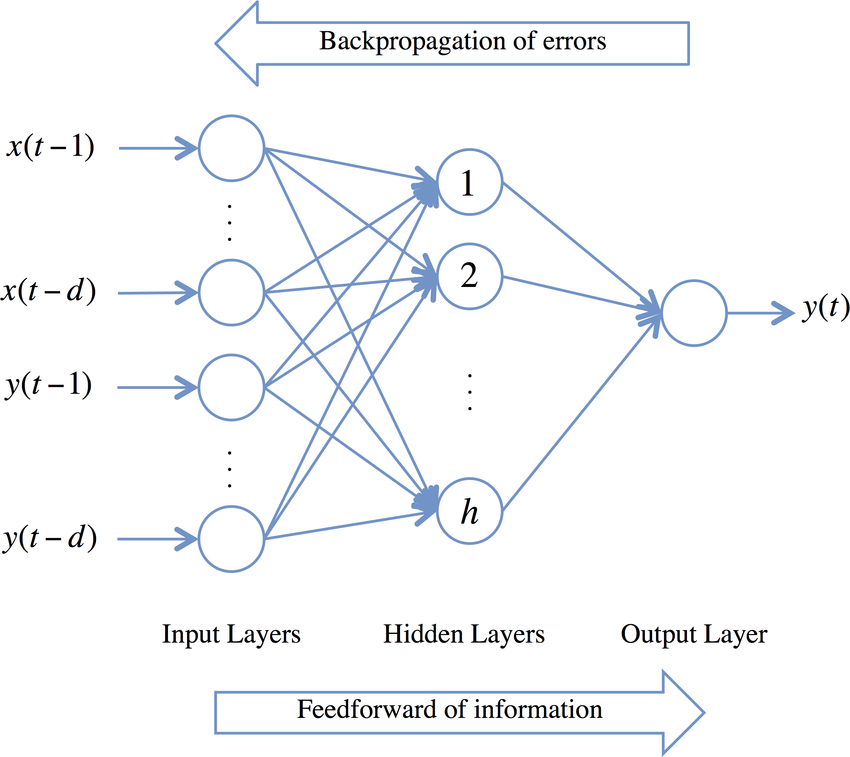
\includegraphics[width=13cm,height=10cm]{nn}
	\end{center}

	\caption{\\~\\Figura: Schema semplificato di Backpropagation Neural Nework. Una Neural Network è un'interconnessione di un gruppo di nodi chiamati neuroni. Ha un livello di neuroni di input, un numero variabile di livelli intermedi (\textit{hidden layers}) e un livello di output. I segnali si propagano dagli input attraverso gli strati nascosti, fino all'output. Nel caso di backpropagation, durante il training, i pesi, e gli altri parametri della rete sono modificati propagando l'errore dall'output verso gli input}.
\end{fig}

\\~\\In letteratura è stato dimostrato che Neural Network offre la capacità di prevedere le direzioni del mercato in modo più preciso rispetto ad altre tecniche esistenti. La capacità delle Neural Network di scoprire relazioni non lineari tra le coppie input / output di training li rendono ideali per la modellazione con sistemi dinamici non lineari come i mercati azionari \cite{nn1}. Uno dei vantaggi è la capacità di poter apprendere le relazioni attraverso i dati stessi, anziché considerare la forma funzionale della relazione. Dato che le Neural Network sono conosciute come approssimatori universali, ogni relazione può essere modellata con un qualsiasi grado di precisione, quando sufficienti dati vengono forniti per la modellazione. Forniscono, inoltre, un livello di tolleranza al rumore ed alla rappresentazione incompleta dei dati.\\
Un altro vantaggio è che Neural Network ha proprietà di apprendimento adattive non lineari, non parametriche, ed ha un effetto molto pratico nella modellazione e predizione. La loro natura non lineare mostra un grande potenziale per risolvere molti problemi complessi. A causa delle caratteristiche di cui sopra dei mercati azionari, le Neural Network possono essere applicate alla predizione del mercato azionario. In primo luogo, è difficile modellare i dati di borsa a causa della loro complessità, quindi, il modello non lineare è vantaggioso. E? spesso richiesto, inoltre, un ampio set di serie temporali correlate in input per modellare uno specifico asset.\\~\\Parlando, invece, degli aspetti negativi, Neural Network ha il problema della scatola nera, cioè che non rivela il senso ed il valore di ogni variabile ed il modo in cui pesa le indipendenti variabili \cite{nn1}. Dato che il ruolo individuale di ogni variabile non può essere determinato, è impossibile da capire come la rete produce il prezzo futuro delle azioni.\\
Un altro grosso problema, con le Neural Network, è il sovrallenamento. Quando le reti si adattano troppo bene ai dati, il sistema perde la capacità di generalizzare. Siccome la capacità di generalizzazione è fondamentale per prevedere lo stock futuro prezzi, il sovrallenamento è un problema serio. Questo, di solito, avviene per due motivi principali: quando le Neural Network hanno troppi nodi o periodi di training troppo lunghi (\textit{epoch} \footnote{Un epoch è quando un \textit{intero} dataset di training viene passato in avanti ed indietro attraverso la rete neurale solo una volta per allenarla.}). Il sovrallenamento, tuttavia, può essere prevenuto eseguendo procedure di test e train o \textit{cross validation}.\\~\\Per quanto riguarda il rumore tremendo, e le caratteristiche non stazionarie nei dati di borsa, Lawrence et al. \cite{nn1} ha sottolineato che, quando l'addestramento delle Neural Network è difficile per dati molto rumorosi, le reti cadono in una soluzione ingenua come prevedere sempre l'output il più comune. Le Neural Network, inoltre, hanno alcune limitazioni nell'apprendimento dei pattern quando i dati di input hanno un'alta dimensionalità. Dash e Liu \cite{2} pongono l'accento sulla selezione delle \textit{feature}\footnote{Nell'apprendimento automatico e nel riconoscimento di pattern, una "feature" (caratteristica) è una proprietà misurabile individuale o caratteristica di un fenomeno osservato. La scelta di feature informative, discriminanti ed indipendenti è un passaggio cruciale per algoritmi efficaci nel riconoscimento, nella classificazione e nella regressione dei modelli. Il concetto di feature è correlato a quello della variabile esplicativa utilizzata nelle tecniche statistiche come la regressione lineare.} e suggeriscono che ridurre il il numero di variabili in input, a volte, porta ad un miglioramento di prestazioni del modello per un determinato set di dati. La riduzione e trasformazione delle feature irrilevanti, o ridondanti, possono ridurre il tempo di esecuzione e produrre risultati più generalizzati \cite{2}.\\~\\ Ricerche recenti tendono a utilizzare diverse tecniche di AI \textit{ibride}\footnote{Un sistema intelligente \textit{ibrido} indica un sistema software che impiega, in parallelo, una combinazione di metodi e tecniche provenienti da diversi sottocampi di intelligenza artificiale, come, ad esempio: \textit{neuro-fuzzy systems}, \textit{evolutionary neural network}, \textit{genetic fuzzy systems}, \textit{reinforcement learning} con \textit{fuzzy}, \textit{neural}, o \textit{evolutionary}, etc.}. Hiemstra \cite{11} ha proposto \textit{sistemi esperti fuzzy}\footnote{La logica fuzzy è una logica in cui si può attribuire a ciascuna proposizione un grado di verità diverso da 0 e 1, e compreso tra di loro. È una logica polivalente, ossia un'estensione della logica booleana. Con grado di verità, o valore di appartenenza, si intende quanto è vera una proprietà: questa può essere, oltre che vera (= a valore 1) o falsa (= a valore 0), come nella logica classica, anche parzialmente vera e parzialmente falsa.} per prevedere i rendimenti del mercato azionario. Suggerì che, combinando le Neural Network con la logica fuzzy, si possa catturare la complessità del mapping funzionale e non è richiesta la specifica della funzione da approssimare. Tsaih et al. \cite{41} ha integrato la tecnica basata su regole e le Neural Network per prevedere la direzione di cambio dello stock S\&P 500\footnote{L'indice Standard \& Poor 500, noto come S\&P 500 o semplicemente S\&P, è stato realizzato da Standard \& Poor's nel 1957 e segue l'andamento di un paniere azionario formato dalle 500 aziende statunitensi a maggiore capitalizzazione.} \textit{futures}\footnote{I futures (future contracts) sono contratti a termine standardizzati per poter essere negoziati facilmente in una borsa valori, e sanciscono l'impegno ad un acquisto differito ad un prezzo prefissato. } su base giornaliera.

\subsubsection{Support Vector Machine}
Support Vector Machine (SVM) basato su teoria dell'apprendimento statistico, è stato sviluppato da Vapnik \cite{44} ed i suoi colleghi alla fine degli anni '70. È diventato un argomento caldo di studio intensivo grazie al suo successo applicato a compiti di classificazione e regressione, soprattutto nella previsione di serie temporali e applicazioni correlate alla finanza \cite{46}. Support Vector Machine è una tipologia molto specifica di algoritmi di apprendimento caratterizzato dal controllo della capacità della funzione di decisione, l'uso delle funzioni del kernel e la dispersione della soluzione \cite{43}. Fondato sulla teoria del \textit{principio di minimizzazione del rischio strutturale}\footnote{La minimizzazione del rischio strutturale (SRM) è un principio induttivo in uso nell'apprendimento automatico. Comunemente, in machine learning, un modello generalizzato deve essere selezionato a partire da un set di dati finito, con il conseguente problema di overfitting: il modello diventa troppo fortemente adattato alle particolarità dei dati di training e generalizza male i nuovi dati. Il principio SRM affronta questo problema bilanciando la complessità del modello con il suo successo nell'adattare i dati di addestramento.}, in cui stima una funzione minimizzando l'errore di generalizzazione, Support Vector Machine si dimostra alla fine molto resistente al problema del sovrallenamento (\textit{overtraining}), raggiungendo un ottimo risultato nella generalizzazione.\\ Un'altra proprietà chiave è che addestrare Support Vector Machine equivale a risolvere un problema di programmazione linearmente vincolato. Pertanto, la soluzione di Support Vector Machine è relativamente unica e globalmente ottimale, a differenza del training delle Neural Network, che richiede un'ottimizzazione non lineare con pericolo di rimanere bloccati ai minimi locali.\\~\\ 

\begin{fig}
	\begin{center}
		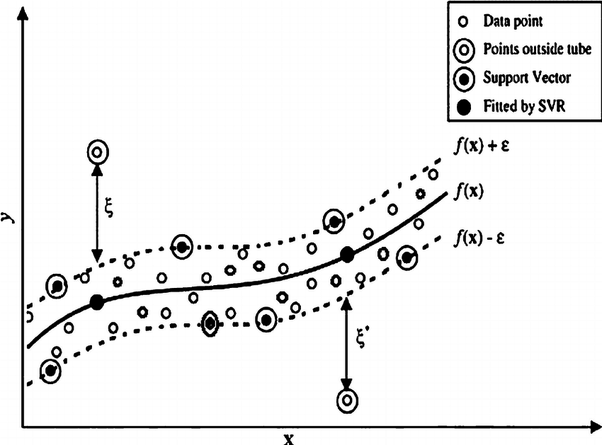
\includegraphics[width=12cm,height=8cm]{svm1}[h]
	\end{center}
	\caption{\\~\\Figura: Support Vector Machine applicato al compito di regressione: nel caso di funzioni non lineari, queste vengono mappate in spazi multidimensionali per mezzo di metodi kernel. Dopodichè viene applicata la tecnica dei vettori di supporto per delineare gli estremi della funzione da approssimare. Si ottiene un'approssimazione che, in ogni punto, discosta al massimo di \varepsilon \text{ dai valori noti della funzione.}}
\end{fig}

\\~\\Di recente, diverse applicazioni di Support Vector Machine a problemi di previsioni finanziarie sono state documentate \cite{15}\cite{38}\cite{39}. Uno degli studi ben noti che utilizzano Support Vector Machine per la predizione del mercato è stato eseguito da Kim \cite{15}. Ha applicato Support Vector Machine alle previsioni finanziarie e confrontato il risultato rispetto a \textit{backpropagation}\footnote{In machine learning, in particolare deep learning, backpropagation è un algoritmo ampiamente utilizzato nel training di reti neurali feedforward per l'apprendimento supervisionato. L'algoritmo di backpropagation funziona calcolando il gradiente della funzione di perdita rispetto a ciascun peso della \textit{chain rule}, calcolando il gradiente uno strato alla volta, ripetendo all'indietro dall'ultimo strato per evitare calcoli ridondanti di termini intermedi.} Neural Network e Case Based Reasoning (CBR). I risultati sperimentali hanno mostrato che Support Vector Machine ha avuto performance migliori di Neural Network e Case Based Reasoning. Poiché Support Vector Machine si basa sul principio di minimizzazione del rischio strutturale, la generalizzazione implementata risulta migliore rispetto alle tecniche tradizionali.

\subsubsection{Case Based Reasoning}
\begin{fig}
	\begin{center}
		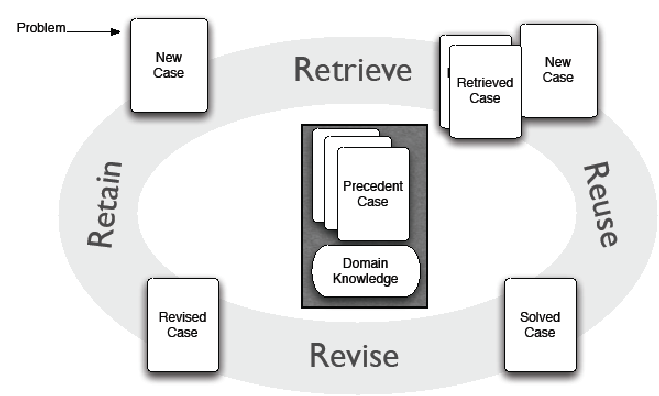
\includegraphics[width=13cm,height=8cm]{cbr}
	\end{center}

	\caption{\\~\\ Figura: Il processo di risoluzione di nuovi problemi basandosi sulle soluzioni di problemi anteriori, esempio generale di algoritmo CBR. Dato un problema, recuperare in memoria dei casi rilevanti per risolverlo (\textit{Retrieve}). Adattare la soluzione del caso precedente al problema attuale (\textit{Reuse}). Avendo mappato la soluzione precedente al caso attuale, bisogna provare la nuova soluzione e, se necessario, rivedere la nuova soluzione (\textit{Revise}). Dopo che la soluzione è stata adattata al problema attuale, memorizzare l'esperienza come nuovo caso (\textit{Retain})}.
\end{fig}

\\~\\Sebbene le Neural Network offrano capacità di apprendimento relativamente buone rispetto ad altre tecniche, non possono sempre esplicitare il perché arrivano ad una particolare soluzione. Non garantiscono, inoltre, sempre una soluzione completamente certa, non assicurano di arrivare ripetutamente alla stessa soluzione dato lo stesso dataset di training, né possono garantire di trovare la soluzione ottimale\cite{40}. Tuttavia, a differenza delle reti neurali, in genere i \textit{sistemi esperti}\footnote{Un sistema esperto è un programma che cerca di riprodurre le prestazioni di una o più persone esperte in un determinato campo di attività, ed è un'applicazione o una branca dell'intelligenza artificiale. Sono spesso implementati attraverso euristiche o fuzzy logic e si dividono in due categorie principali: basati su regole e basati su alberi.} forniscono spiegazioni per le loro soluzioni. I sistemi esperti acquisiscono, principalmente, la conoscenza da individui esperti nell'ambito. Le organizzazioni hanno conoscenze collettive e competenze che hanno accumulato nel corso degli anni. Queste conoscenze possono essere acquisite, ed archiviate, utilizzando Case Based Reasoning. È una tecnica di ragionamento che riutilizza i casi passati per trovare una soluzione al nuovo problema. Case Based Reasoning non solo acquisisce la conoscenza dell'organizzazione, ma fornisce anche spiegazioni per le soluzioni derivate. Per questa ragione, è comunemente applicato a molti problemi.\\~\\ Kim \cite{17} ha proposto un nuovo modello ibrido di Genetic Algorithm e Case Based Reasoning per la previsione del mercato azionario. Dal suo studio preliminare, ha scoperto che la scelta del peso delle feature, e del sottoinsieme delle stesse, è molto importante per migliorare le prestazioni delle predizioni del sistema. Ha, quindi, usato Genetic Algorithm come metodo di selezione del sottoinsieme di feature nel sistema Case Base Reasoning. Ha confrontato i risultati di quattro diversi modelli per testare l'efficacia del modello proposto. I modelli a confronto sono: CBR convenzionali (COCBR), pesatura delle feature utilizzando Genetic Algorithm per CBR (FWCBR), selezione delle feature usando Genetic Algorithm per CBR (FSCBR) e ottimizzazione simultanea usando Genetic Algorithm per CBR (SOCBR). I risultati empirici hanno mostrato che SOCBR raggiunge una precisione di previsione superiore rispetto a COCBR, FWCBR e FSCBR. Kim ha concluso che il modello ibrido di GA e CBR offre un valido approccio alternativo alla previsione del mercato azionario.

\subsubsection{Informazione sugli eventi}
Nei mercati azionari, ci sono molti fattori che possono influenzare il prezzo dei titoli. Questi fattori possono essere derivati dai comunicati stampa sulle piccole aziende o dalle notizie delle superpotenze dell'economia mondiale. Questi episodi sono chiamati \textit{events} \cite{29}. Il motivo principale per cui incorporare conoscenza degli eventi nella previsione del mercato azionario si basa sul presupposto che il prezzo futuro di un'azione dipende in parte da vari aspetti politici ed eventi internazionali, oltre ai vari indicatori economici. Pertanto, molti studi hanno utilizzato informazioni sugli eventi (fattori qualitativi) nonché dati quantitativi nella previsione dei mercati azionari.\\~\\ Uno degli studi popolari che utilizzano la conoscenza degli eventi e la \textit{conoscenza pregressa} è stato realizzato da Kohara et al. \cite{know-nn2}. I ricercatori hanno incorporato la conoscenza preliminare nella previsione di mercato, come informazioni sui giornali su eventi nazionali ed esteri. La conoscenza dell'evento è estratta dai titoli dei giornali in conformità con alcune conoscenze preliminari. La conoscenza pregressa è l'informazione che deriva da precedenti esperienze, pertanto, in base alla conoscenza precedente, decisioni differenti possono essere prese se un evento particolare può influenzare positivamente o meno le tendenze del mercato azionario.\\~\\\\
\begin{fig}
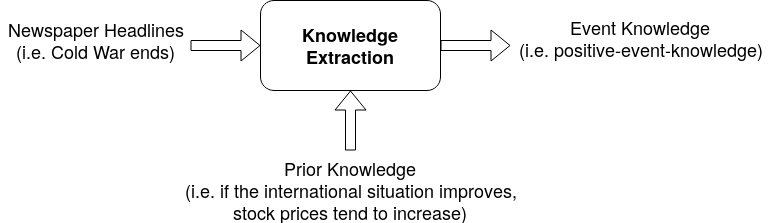
\includegraphics[width=\linewidth]{prior_knowledge}
\caption{\\~\\Figura: Estrazione di conoscenza sugli eventi: basandosi sulle notizie di giornale e avendo coscienza dell'impatto che possono avere certi eventi sull'economia, è possibile stimare se un certo evento può influire positivamente o negativamente sul mercato.}
\end{fig}

\\~\\Kohara et al. \cite{know-nn2} hanno selezionato diversi indicatori economici (tasso di interesse, prezzo del petrolio grezzo e media dei prezzi di chiusura di New York Dow Jones) e forniti insieme alla conoscenza degli eventi come dati di training per Neural Network. I loro risultati sperimentali hanno mostrato che incorporare la conoscenza di eventi ha migliorato la capacità di previsione delle Neural Network, riducendo il tasso di errore del 5\% del livello di significatività. Intanto, risulta cruciale \textit{come} incorporare l'impatto delle informazioni sulle notizie nei modelli di serie storiche. Maheu e McCurdy \cite{26} hanno specificato un modello GARCH\footnote{In econometria, un modello autoregressivo a eteroschedasticità condizionata generalizzato o modello GARCH (Generalized AutoRegressive Conditional Heteroskedasticity) è un modello utilizzato nell'analisi delle serie storiche. È una funzione dei valori assunti dal processo agli istanti precedenti.} con salti per serie di ritorno, che può essere direttamente misurato dai dati dei prezzi. Si è supposto che il processo latente delle notizie abbia due componenti separati, eventi di cronaca normali ed insoliti. Queste differenti notizie sono identificate attraverso il loro impatto sulla \textit{volatilità} del rendimento\footnote{In finanza, la volatilità è una misura della variazione percentuale del prezzo di uno strumento finanziario nel corso del tempo. Corrisponde alla \textit{Deviazione standard}. Di solito indica il livello di rischio associato ad un titolo: possedendo un titolo più volatile si è più esposti alle oscillazioni del suo valore.}.\\~\\ I modelli precedenti forniscono quadri generali per incorporare gli impatti delle notizie di giornale. Questi metodi non forniscono, però, un approccio per la distinzione delle notizie influenti o significative per un determinato titolo, a fronte di migliaia di articoli di ogni genere. Questi metodi,peratnto, nella pratica, non possono garantire un miglioramento significativo. \\~\\
In letteratura, un certo numero di ricercatori ha affermato che i prezzi delle azioni sono significativamente correlati con le informazioni relative agli eventi e molti hanno tentato di utilizzare sia informazioni sugli eventi che dati numerici di serie temporali come dati in input. Fawcett e Provost \cite{4} hanno formulato il problema di previsione del mercato come un'attività di monitoraggio della relazione tra le notizie ed i prezzi delle azioni. Fung et al. \cite{news-nn} hanno proposto un sistema che prevede il cambiamenti nell'andamento del mercato analizzando l'influenza di informazioni qualitative (notizie di giornale). In particolare, hanno studiato l'impatto immediato delle notizie sulle serie storiche basate sull'ipotesi di mercato efficiente. Hanno proposto un nuovo algoritmo statistico di \textit{segmented regression}\footnote{La regressione segmentata (segmented regression), nota anche come piecewise regression o broken-stick regression, è un metodo di analisi di regressione in cui la variabile indipendente è suddivisa in intervalli ed un segmento di linea separato è adattato a ciascun intervallo. L'analisi di regressione segmentata può anche essere eseguita su dati multivariati partizionando le varie variabili indipendenti. La regressione segmentata è utile quando le variabili indipendenti, raggruppate in gruppi diversi, mostrano relazioni diverse tra le variabili in queste regioni.} per identificare le tendenze nelle serie temporali. In letteratura viene sempre più riconosciuta l'incorporazione della conoscenza pregressa e conoscenza degli eventi nei modelli di previsione come Neural Network.

\subsubsection{Informazione sugli eventi nel Web}
L'evoluzione di Internet, con l'infrastruttura di informazioni globale, ha provocato un'esplosione della quantità di informazioni disponibili. Enormi moli di dati relativi a eventi che possono avere grande influenza sul mercato azionario sono disponibile sul web. Considerando che i giornali vengono aggiornati una o due volte al giorno, le fonti di notizie in tempo reale sono aggiornate frequentemente quasi istantaneamente. Queste informazioni non contengono solo notizie globali e regionali ma anche citazioni preziose di influenti banchieri, politici e analisti finanziari. Le informazioni che consistono in notizie o citazioni sono viste come principali motori del mercato delle obbligazioni, delle valute e azionario nel mondo. Hong e Han \cite{13} hanno affermato che, con l'aumento della popolarità di Internet, molti giornali espanderanno i loro servizi fornendo notizie sul web, per essere più competitivi e aumentare il profitto. Le notizie includono articoli sulla situazione politica, le condizioni sociali, eventi internazionali, politiche governative, psicologia dei trader e così via; informazioni che vediamo e comprendiamo attraverso Internet. Tali informazioni sono formulate sotto forma di testo, indicati come documenti, quindi tecniche di \textit{text mining}\footnote{Text mining è la scoperta da parte del computer di informazioni nuove, precedentemente sconosciute, estraendo automaticamente informazioni da diverse fonti di testo.	È il processo di estrazione di informazioni di alta qualità dal testo. Le informazioni sono in genere derivate dall'elaborazione di modelli e pattern attraverso mezzi come l'apprendimento automatico e statistico di pattern. L'estrazione del testo di solito comporta il processo di strutturazione del testo di input (\textit{parsing}), estrazione di pattern all'interno dei dati strutturati e, infine, la valutazione e l'interpretazione dell'output.} sono necessarie.\\~\\
Hong e Han \cite{13} hanno introdotto un sistema automatizzato (KBNMiner) che acquisisce conoscenza degli eventi da Internet, per la predizione dei tassi di interesse. Questo studio
mostra una chiara idea di conoscenza dell'evento usando un sistema automatizzato. KBNMiner è progettato per adottare una base di conoscenza preliminare, che viene vista come "conoscenza esperta", come base su cui raccogliere informazioni sugli eventi da Internet automaticamente e quindi applicare le informazioni a un modello di Neural Network per la previsione dei tassi di interesse. Ciò che si distingue in questo studio è che la tecnica di web mining che hanno applicato per la previsione dei tassi di interesse può anche essere utilizzata per previsione del mercato azionario.

\subsubsection{Lavori futuri}
In questa sezione si sono esaminati i recenti sviluppi dei modelli di previsione del mercato azionario. Confrontando vari modelli di predizione, si è scoperto che le Neural Network offrono l'abilità di prevedere le direzioni del mercato in modo più accurato rispetto ad altre tecniche esistenti. La capacità di Neural Network di imparare relazioni non lineari dalle coppie di input / output di training consente loro di modellare sistemi dinamici non lineari, come i mercati azionari, più precisamente \cite{23}.\\Anche altri modelli come Support Vector Machine e Case Based Reasoning sono diventati popolari nella previsione del mercato azionario. Support Vector Machine ha mostrato la sua corretta applicazione nei problemi di classificazione e di regressione, in particolare nella previsione di serie storiche e applicazioni finanziarie correlate \cite{46}. Case Based Reasoning è una tecnica di ragionamento che riutilizza casi passati per trovare una soluzione al nuovo problema. Case Based Reasoning cattura la conoscenza e la competenza di un'organizzazione fornendo spiegazioni per le soluzioni derivate. Per questa ragione, Case Based Reasoning è comunemente applicato a molti problemi.\\ Studiando diversi punti chiave dei mercati azionari, inoltre, si è scoperto che molti ricercatori hanno riconosciuto che fattori qualitativi come effetti politici ed eventi internazionali possono avere un impatto significativo sui prezzi delle azioni. È stato esaminato che Neural Network basate sia sui fattori quantitativi che qualitativi sono di gran lunga superiori a quelle basate solo su fattori quantitativi. Il web, inoltre, è considerato come la principale fonte di notizie sugli eventi per la predizione del mercato azionario, contenendo informazioni sugli eventi più recenti e latenti. Pertanto, per prevedere il mercato, tecniche di web mining sono necessarie per avere una maggiore accuratezza e per fare predizioni in un tempo più breve.\\~\\ Per ulteriori ricerche, in primo luogo, un database contenente conoscenza preliminare dovrebbe essere costruito analizzando eventi storici nei mercati azionari. Sulla base delle conoscenze precedenti, verrà sviluppato lo schema di attribuzione di peso degli eventi e ciascun evento dovrebbe essere pesato di conseguenza. Il modello proposto che incorpora i pesi degli eventi nei dati numerici delle serie temporali, infine, dovrebbe essere confrontato empiricamente con altri modelli.

\newpage
\section{Sentyment}
A differenza degli algoritmi appena citati, Sentyment si concentra sulla creazione di strategie di investimento, invece che la previsione dell'andamento nel tempo di un particolare titolo azionario. Gestisce contemporaneamente più asset. Non si può paragonare agli algoritmi nello stato dell'arte sul piano della precisione di previsione, perchè la funzione che cerca di massimizzare non è la stessa delle AI accademiche. Questo software commerciale ha come scopo il rispetto delle politiche scelte dall'utente in merito a propensione al rischio e interessi personalizzati e la massimizzazione del guadagno attraverso l'ottimizzazione di alcuni indicatori come, appunto, il guadagno prodotto dalla strategia o il numero di operazioni vincenti.\\ A differenza degli algoritmi sopra citati, in cui lo scopo è \textit{prevedere quale valore avrà la funzione} in un certo istante, ciò che trova Sentyment è invece \textit{quale operazione fra buy, sell o hold conviene eseguire} al fine di massimizzare il guadagno, in un certo istante.\\~\\
Ciò premesso, è comunque ovvio il fatto che il sistema abbia una certa capacità di previsione del mercato, di identificazione dei pattern ricorrenti o addirittura un'integrazione di informazioni sugli eventi. Per poter competere con gli altri sistemi presenti sul mercato deve fare sicuramente uso di una o più fra le tecniche descritte in questo capitolo. La AI, tuttavia, verrà trattata come una \textit{black-box} e non saranno, quindi, rivelati dettagli sulla sua implementazione, ma verranno considerati soltanto gli input e gli output.\\~\\ L'analisi comparativa con altri sistemi risulta, quindi, difficile in quanto gli obiettivi dei software sono differenti. È comunque possibile misurare rispetto ad indicatori assoluti o comparare fra loro le diverse AI che compongono Sentyment.

\subsection{Cenni all'architettura}
Sentyment è il prodotto di un'azienda milanese che opera nel settore informatico-finanziario. Nexid Edge è un ramo del gruppo NEXiD votato per perseguire l'innovazione tecnologica e sviluppare soluzioni di digital business rivoluzionarie. SentYment è la nuova Business Unit dedicata all'intelligenza artificiale.\\
L'obiettivo è offrire alle organizzazioni un accesso senza pari a tecnologie all'avanguardia che uniscono il meglio della tecnologia e dell'imprenditorialità per elevare la saggezza collettiva. Al momento, grazie all'intensa collaborazione con Nexid Finance, Nexid Edge è attiva nel fornire progetti di consulenza digitale end-to-end, per offrire ai clienti un'esperienza di \textit{augmented consulting}. \footnote{Nexid, Srl. URL: https://nexid.it/}\\
In questo documento, tuttavia, si fa riferimento a "Sentyment" intendendo l'applicazione sviluppata, e non la divisione AI di Nexid.
\\~\\
Essendo il fine ultimo della tesi l'inserimento un nuovo modulo operativo in Sentyment, è necessario prendere familiarità con il software ed i dati che tratta.\\
L'applicazione di intelligenza artificiale era già esistente ed in grado di raccogliere dati da Kraken e produrre le strategie, ma mancava di un'architettura modulare, di componenti separati che assolvessero a ruoli precisi e definiti e di un'interfaccia ad API per interrogare il sistema in esecuzione. Era, quindi, necessario sviluppare da zero \textit{data module} e \textit{coordinator} e permettere l'integrazione del resto del sistema già esistente nella nuova architettura a moduli. Era, inoltre, richiesto lo sviluppo della nuova AI di controllo, supervisore che scegliesse la migliore fra le AI in esecuzione.\\
Tutti i moduli del sistema sono scritti in Python3, comprese le AI stesse. Alcune loro parti sono state riscritte in Cython e Go per migliorare le prestazioni.
\\~\\
	\begin{fig}
	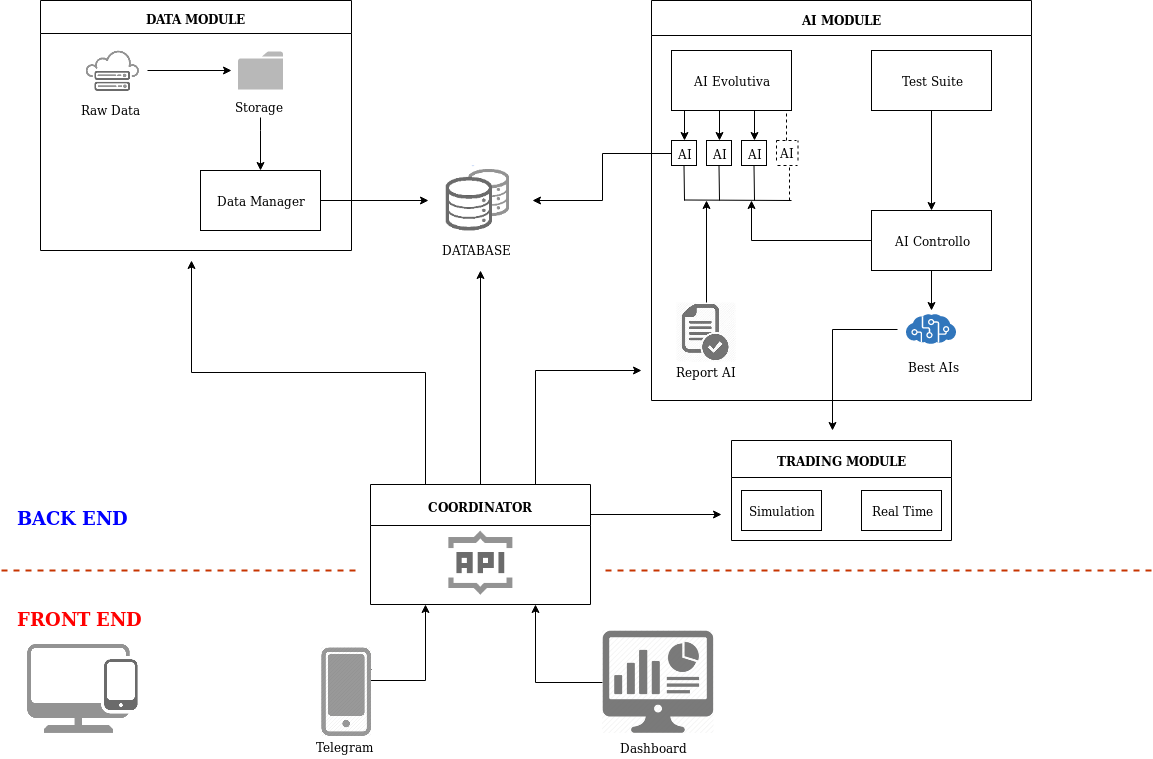
\includegraphics[width=\linewidth]{Sentyment}
	\caption{\\~\\Figura: Architettura di Sentyment. Nei riquadri sono mostrati i quattro principali componenti, suddivisi al loro interno in ulteriori sotto-moduli. Il grafico è diviso in \textit{front-end} e \textit{back-end}, che rappresentano rispettivamente le interfacce esposte all'utente utilizzatore del sistema, e la parte di logica non accessibile dall'esterno}
\end{fig}
\\~\\

Verranno ora brevemente presentati i componenti di Sentyment.
\begin{itemize}
	\item \textit{data module} raccoglie i record di trade raw tramite le API Kraken, gestisce la creazione e scrittura delle candele OHLCV e permettere l'accesso a tutti i dati ed i database da parte degli altri componenti. I sotto-moduli si spartiscono i compiti: quando i dati di trade sono scaricati e salvati su uno storage temporaneo da \textit{raw data}, allora \textit{data manager} li copia sul database permanente e, in automatico, scatta la creazione delle nuove candele OHLCV, che sono create allo scoccare della nuova ora, a partire dai dati appena scaricati (o minuto/giorno, a seconda delle configurazioni scelte). Le nuove candele create, infine, sono inserite nel database.
	\item \textit{coordinator} implementa le interfacce esposte per il controllo e l'interrogazione dello stato di Sentyment. È l'unico punto di accesso al sistema in esecuzione. Tramite delle API esposte su server è possibile conoscere quali asset sono attualmente in fase di scaricamento e le informazioni riguardo le configurazioni delle candele che si vogliono creare; è, inoltre, possibile impostare i timeframe delle candele (orarie, giornaliere), attivare o disattivare i download dati e forzare la creazione di specifiche candele.
	\item \textit{AI module} è la parte preesistente di intelligenza artificiale. Contiene le numerose AI che creano le strategie di investimento ed il supervisore che sceglie la migliore fra queste, a intervalli fissati. È, inoltre, presente un modulo che crea report che descrivono l'andamento delle AI, i dati che stanno processando e le statistiche calcolate per ognuna di esse, per misurarne la performance online.
	\item \textit{trading module} si occupa di seguire le strategie create dalle AI per effettuare direttamente operazioni di acquisto e vendita tramite le API di Kraken. È collegato ad un portafoglio Kraken che contiene un certo budget ed è libero di fare trading. Oltre ad agire sul mercato vero, le AI operano anche in un ambiente simulato che permette di riprodurre, e monitorare, quale sarebbe stato il loro comportamento nel mercato reale, o in nuovi mercati non ancora raggiunti, al fine di calcolare ulteriori statistiche e tracciare l'evoluzione delle AI.
\end{itemize}

Come già accennato, sono stati sviluppati \textit{data module} e \textit{coordinator}, ridisegnando la preesistente architettura di Sentyment ed integrando gli altri componenti. Durante la riprogettazione, si sono potute scegliere liberamente la logica di implementazione e le tecnologie da impiegare, con la restrizione di dover utilizzare Python3, con \textit{sqlalchemy}\footnote{SQLAlchemy è un toolkit SQL open-source e object-relational mapper (ORM) per Python} come \textit{ORM}\footnote{l'Object-Relational Mapping (ORM) è una tecnica di programmazione che favorisce l'integrazione di sistemi software aderenti al paradigma della programmazione orientata agli oggetti con sistemi RDBMS (Relational Database Management System). Un prodotto ORM fornisce, mediante un'interfaccia orientata agli oggetti, tutti i servizi inerenti alla persistenza dei dati, astraendo, nel contempo, le caratteristiche implementative dello specifico RDBMS utilizzato.} e \textit{flask}\footnote{Flask è un micro framework web scritto in Python. Ha un nucleo semplice ma estendibile: ci sono, ad esempio, estensioni per la validazione delle form, la gestione del caricamento dei file, varie tecnologie di autenticazione ed altro} per implementare il server e le API.\\
Prima di sviluppare la AI supervisore, sono state testate le AI singolarmente attraverso alcune metodologie di test che saranno descritte di seguito. È stato svolto un lavoro di analisi dei dati prodotti dalle AI, confrontandoli con alcune strategie di base e con altre intelligenze artificiali sviluppate al fine di misurarne le prestazioni e, solo dopo, le AI sono state confrontate fra di loro. I metodi ritenuti migliori per il confronto sono stati scelti in seguito ad un'analisi del contesto ed alla natura finanziaria dei dati.

\begin{fig}
	\begin{center}
		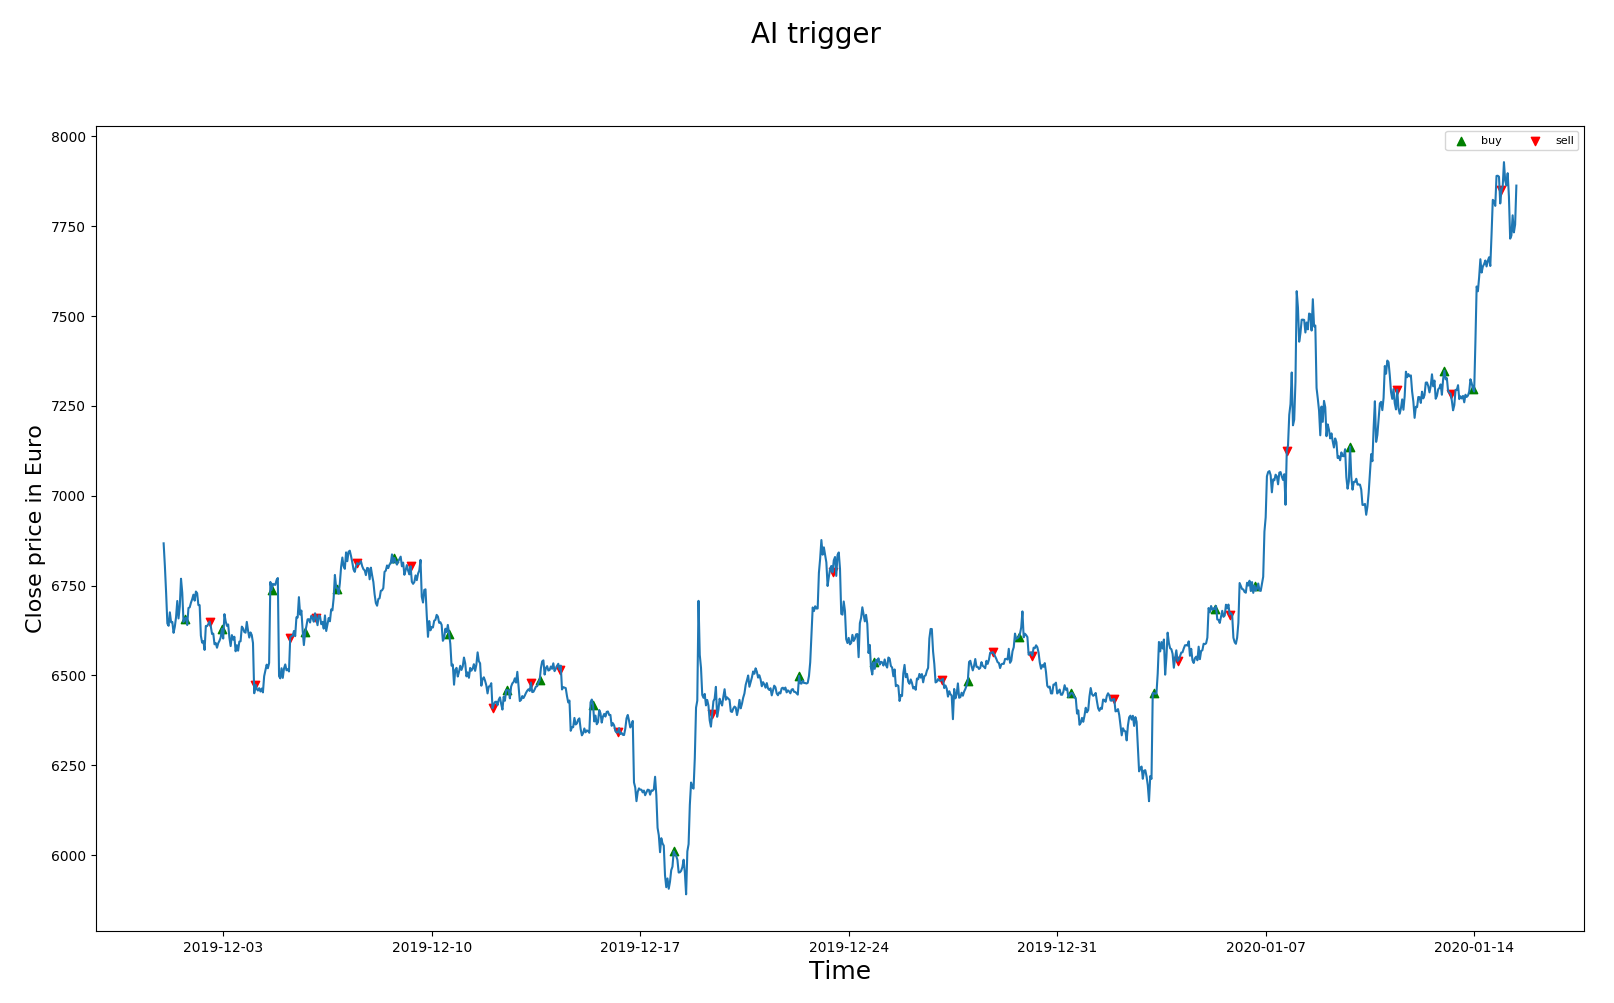
\includegraphics[width=\linewidth]{ai_trigger_big}
	\end{center}
	\caption{Figura: esempio dei \textit{trigger} generati da una delle AI di Sentyment. Il grafico fa riferimento ai prezzi di chiusura del ticker BITCOIN-EURO relativi ad un certo periodo temporale, da fine 2019 a inizio 2020. Come si può notare, la AI cerca quasi sempre di effettuare buy nei punti di minimo, mentre i segnali di sell sono spesso nei punti più alti che seguono un picco basso.}
\end{fig}

\subsection{Strumenti e tecnologie utilizzati}
Sentyment è quasi totalmente scritta in Python3, tranne per alcune parti in cui si ha bisogno di elevate performance che sono, quindi, state riscritte in Cython\footnote{Cython è un linguaggio di programmazione che mira ad essere un superset del linguaggio di programmazione Python, progettato per fornire prestazioni di tipo C con codice scritto principalmente in Python con sintassi aggiuntiva opzionale ispirata al C}. Queste comprendono, ad esempio, gran parte del codice delle AI, ma non solo.\\
Si fa uso estensivo di librerie di analisi dati quali \textit{numpy}\footnote{NumPy è una libreria open source per il linguaggio di programmazione Python, che aggiunge supporto a grandi matrici ed array multidimensionali, insieme ad una vasta collezione di funzioni matematiche di alto livello, per poter operare efficientemente su queste strutture dati.}, \textit{pandas}\footnote{Pandas è una libreria software scritta per il linguaggio di programmazione Python per la manipolazione e l'analisi dei dati. In particolare, offre strutture dati ed operazioni per manipolare tabelle numeriche e serie temporali. Il nome deriva dal termine "panel data", termine econometrico per set di dati che include osservazioni su più periodi di tempo per gli stessi individui.} e \textit{matplotlib}\footnote{Matplotlib è una libreria per la creazione di grafici per il linguaggio di programmazione Python e la libreria matematica NumPy. Fornisce API orientate agli oggetti che permettono di inserire grafici all'interno di applicativi} per visualizzare i grafici dei dati, soprattutto nella parte di sviluppo e analisi.\\
Queste librerie sono i classici strumenti utilizzati nell'analisi dati con Python e sono i più utilizzati; le alternative attualmente presenti non offrono le stesse funzionalità con la medesima efficienza e, per questo, erano anche i \textit{tool} già usati nella prima versione di Sentyment.\\
Pandas, in particolare, permette di importare grandi quantità di dati direttamente da database, o da file, ed è in grado di gestirli in modo efficiente indicizzandoli e garantendo un accesso rapido. Un ampio set di operazioni statistiche sui dati lo rende uno strumento indispensabile in \textit{data science} ed ampiamente utilizzato. Basti pensare ad un AI a cui servono in input moltissimi dati: quando questi sono salvati su database, è facile eseguire piccole letture e query puntuali ed aggregate ma, quando, invece, si ha bisogno di portarne in memoria un gran numero per processarli con funzioni al di là delle potenzialità di \textit{SQL}, serve un ulteriore strumento capace di gestire l'accesso efficiente alla memoria e che offra direttamente queste funzioni di analisi (esempio con funzione \textit{resample} nel Capitolo 3).\\~\\ Il database scelto è di tipo \textit{relazionale}. Si è scelta l'opzione relazionale, invece di \textit{noSQL}, in quanto i dati sono tutti perfettamente strutturati (schema dati in dettaglio nel Capitolo 3): la sorgente principale da cui partono tutte le elaborazioni è rappresentata dai dati di trading \textit{raw} forniti da Kraken. Questi hanno ciascuno un riferimento al \textit{timestamp}, alla tipologia dell'operazione di trade, la quantità di titoli venduti / acquistati ed il loro volume. Sostanzialmente, non servono altre informazioni per la creazione delle candele OHLCV, che sono anch'esse strutturate ed esplicitano \textit{open}, \textit{high}, \textit{low}, \textit{close}, \textit{volume}, \textit{timestamp} finale e altri dati secondari. Le AI lavorano tutte sulle candele e necessitano soltanto degli attributi appena citati.\\~\\
L'unica eccezione, in cui dati non sono perfettamente strutturati, sono le AI. Sono memorizzate come un insieme di parametri che permettono la loro ricreazione in un secondo momento, se necessaria, e sono salvati in formato \textit{JSON}.\footnote{JSON, acronimo di JavaScript Object Notation, è un formato adatto all'interscambio di dati fra applicazioni client/server. È basato sul linguaggio JavaScript, ma ne è indipendente.} Dato che i parametri sono diversi, non strutturati, e con possibilità di molteplici valori nulli, la memorizzazione in JSON, già adottata nella prima versione di Sentyment, sembrava comunque adatta, permettendo una compressione più efficiente dei dati ed un accesso orientato al documento. Di una specifica AI si vogliono conoscere i suoi parametri, ma il nome / \textit{id} della AI é noto: per esempio, in seguito ad un'analisi durante un nuovo ciclo di test / sviluppo, si vuole continuare dalla AI più promettente fra quelle della precedente iterazione e, quindi, si accede al documento che contiene tutti i parametri della AI scelta.\\
I JSON dei parametri delle AI non sono scritti su database, ma sono dei file che risiedono direttamente su file system nelle directory di Sentyment, strutturate in modo da poter accedere ai parametri di una certa AI usando il suo identificativo. In sviluppi futuri, potrebbe essere più adatto l'uso di un database non relazionale per la memorizzazione delle AI, oppure sfruttare i tipi di dato JSON presenti in ormai tutti i RDMBS moderni e, quindi, salvare tutto nello stesso database.\\~\\
Fra i database relazionali è stato scelto \textit{Mysql}\footnote{MySQL o Oracle MySQL è un Relational database management system (RDBMS) composto da un client a riga di comando e un server. È un software libero rilasciato a doppia licenza ed è sviluppato per essere il più possibile conforme agli standard ANSI SQL e ODBC SQL. I sistemi ed i linguaggi di programmazione che supportano MySQL sono molto numerosi.} perché meglio si sposa con l'ORM di \textit{sqlalchemy}.\\~\\
Sqlalchemy permette di manipolare database SQL direttamente da Python. Mappa lo schema tabellare dei dati in uno a oggetti più facilmente processabile dal linguaggio di programmazione scelto, in questo caso Python. Grazie alla tecnologia degli ORM, il modello dei dati è sempre disponibile come classe del linguaggio e risulta, quindi, più comodo il loro accesso e manipolazione: ora si lavora con collezioni di oggetti, invece che con un semplice elenco di record contenenti alcuni campi.\\
L'ORM mette anche a disposizione un motore di astrazione per le \textit{query}. Tramite un modello ad API le query eseguite in Python sono tradotte nel dialetto SQL del DBMS sottostante. Al programmatore resta il compito di scrivere le query usando l'\textit{expression language}\footnote{Expression Language (EL) è un linguaggio per creare una rappresentazione interpretabile di conoscenze specifiche. In questo caso, è un linguaggio creato da sqlalchemy appositamente per rappresentare query SQL nel linguaggio di Python.} di sqlalchemy, il sistema usato per rappresentare strutture dei database relazionali e espressioni usando Python.\\~\\
\textit{Flask}, infine, è un microframework per Python ed implementa \textit{coordinator}, il web server che espone le informazioni disponibili sullo stato di esecuzione di Sentyment. È molto minimalista, se mantenute le impostazioni di default, e serve soltanto documenti JSON e non pagine HTML.\\
In futuri sviluppi, le informazioni fornite dal web server in JSON potrebbero essere processate da un'ulteriore componente che le esporrebbe, in modo più user-friendly, attraverso un software di front-end e permetterebbe l'interrogazione di \textit{coordinator}, attraverso le API, in maniera più intuitiva.

\newpage
\begin{fig}
	\begin{center}
		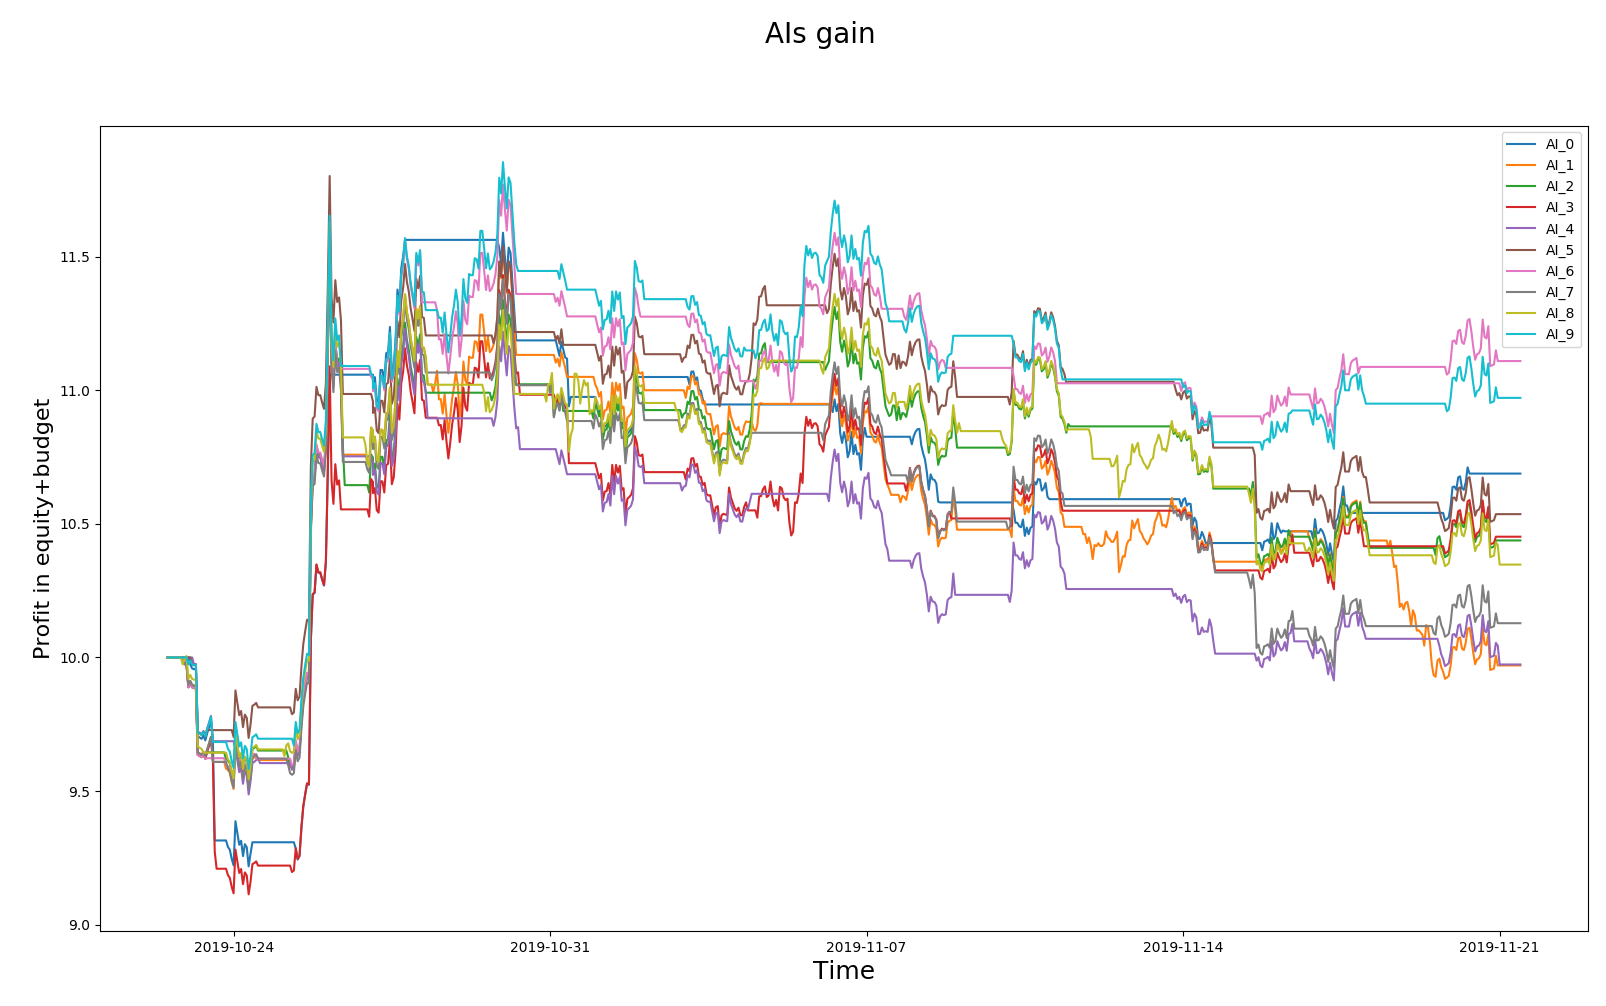
\includegraphics[width=\linewidth]{ai_gains}
	\end{center}
	\caption{Figura: grafico comparativo dei risultati prodotti da 10 differenti AI di Sentyment. È analizzata la funzione guadagno (\textit{gain}, Formula (3)). Questo frammento di dataset, che fa riferimento ai prezzi di BITCOIN-EURO di fine 2019, è particolarmente rappresentativo e compare spesso all'interno dell'intero documento. Si nota come le AI abbiano tutte un comportamento diverso, ma ciascuna con pattern simili: nella settimana del 24 ottobre, a inizio grafico, tutte quante prevedono un aumento del prezzo del titolo e investono capitale, per poi riscontrare un grosso guadagno rappresentato dalla ripida pendenza che tutte le AI mostrano. Seguono altre situazioni simili, in cui le varie linee del guadagno mostrano delle "colline" simili per ciascuna AI.}
\end{fig}

\newpage
\chapter{Elaborazione dati di trading}
\label{cap3}
In questo capitolo si andrà principalmente a descrivere il lavoro svolto dal software di raccolta e gestione dati, \textit{data module}, e alcuni dettagli della sua implementazione. Attraverso l'analisi delle operazioni svolte dal programma si darà anche un ulteriore sguardo ai dati, a come sono organizzati dalla piattaforma di trading e all'interno del software di Nexid, e a come si processano per ottenere un formato utile per l'elaborazione da parte delle AI.\\
Anche se Sentyment comprendeva già una parte di logica di scaricamento dati, in seguito alla sua riorganizzazione è stato necessario riscrivere questa parte di software convertendola interamente in un modulo separato, sempre attivo e pronto a scaricare, con cui si può interagire attraverso \textit{coordinator}. Svolge diverse attività fra cui scaricare grazie alle API di Kraken, creare le candele OHLCV a partire dai dati scaricati e gestire il database.\\~\\
I requisiti dell'applicativo sono i seguenti:
\begin{itemize}
	\item Scaricare dati di trade \textit{raw} per diversi tipi di asset, restando aggiornati in tempo reale con l'arrivo di nuovi
	\item Fornire la possibilità di scaricare dati passati
	\item Creare candele OHLCV a partire dai dati scaricati e poter sceglierne i parametri (lunghezza candela, periodo da considerare)
	\item Salvare su database tutti i dati scaricati
\end{itemize}

\section{Download dati Kraken}
L'input di tutto il sistema sono i dati di trade. Un modulo intero è dedicato alla logica di scaricamento dati, il cui fine è soltanto fornire i suddetti dati alle intelligenze artificiali, che rappresentano la parte principale del software. Tutta l'architettura è orientata al dato; le AI stesse ignorano l'esistenza di \textit{data module}, perché di fatto accedono direttamente al database per prelevare i dati, ignorando chi lo abbia riempito. Un metodo strutturato per "riempire" il database e preparare i dati per le AI è quindi un passo iniziale e fondamentale per tutta l'architettura.\\~\\
Le Web API di Kraken consistono in delle richieste HTTP GET e POST\footnote{GET e POST sono metodi di richiesta supportati da HTTP, un protocollo a livello applicativo usato come principale sistema per la trasmissione d'informazioni sul Web.} e si dividono in \textit{pubbliche} e \textit{private}: tutte le attività svolte da \textit{data module} fanno uso soltanto delle interfacce pubbliche, mentre quelle private, le quali necessitano di un API Key\footnote{Una chiave per API (API Key) è un identificatore univoco utilizzato per autenticare un utente, uno sviluppatore o il programma chiamante un'API. Tuttavia, vengono in genere utilizzati per autenticare un progetto con l'API anziché un utente umano. Spesso si usano per accedere a quelle API che forniscono servizi a pagamento o per superare limitazioni di utilizzo.}, servono per collegare un portafoglio con budget e permettono di eseguire operazioni di acquisto e vendita di titoli. Sono utilizzate soprattutto dal modulo di trading.\\
Le API pubbliche permettono molti tipi di operazioni fra cui, le più usate:
\begin{itemize}
	\item \textbf{Get tradable asset pairs}: elenco di tutti gli asset trattati da Kraken, i \textit{ticker}\footnote{Il ticker è un’abbreviazione che identifica le società che vengono quotate su un mercato finanziario. Quando una società decide di ‘diventare pubblica’, sceglie il tipo di mercato sui cui essere quotata e il ticker di identificazione.}, con associato il nome usato e altre informazioni. Sono 110 in totale le coppie di valute di scambio fra una criptovaluta e la sua controparte in Euro o Dollaro. Alcuni esempi:
	\begin{itemize}
		\item XXBTZEUR: ticker che rappresenta la valuta Bitcoin-Euro (XBT-EUR)
		\item XXBTZUSD: Bitcoin-Dollaro (XBT-USD)
		\item XETHZEUR: Ethereum-Euro (ETH-EUR)
		\item XETHZUSD: Ethereum-Dollaro (ETH-USD)\\
		
		Non ci sono soltanto valute di scambio fra Euro / Dollaro e una criptovaluta, ma bensì anche scambi fra criptovaluta e criptovaluta, come, ad esempio:
		\item ADAETH: valuta di scambio fra le due criptovalute Cardano (ADA)\footnote{Cardano è una piattaforma che gestisce la criptovaluta ADA. Il progetto è guidato dall'ex co-fondatore di Ethereum. Lo scopo di Cardano è creare una piattaforma adatta allo sviluppo di smart contracts e un sistema di pagamento.} ed Ethereum (ETH)
		\item XZECXXBT: Zcash (ZEC)\footnote{Zcash è una criptovaluta che offre privacy e trasparenza selettiva delle transazioni. I pagamenti Zcash sono pubblicati su una blockchain pubblica, ma il mittente, il ricevente e il valore della transazione possono rimanere privati. Come Bitcoin Zcash ha una fornitura fissa totale di 21 milioni di unità.} e Bitcoin (XBT)\\
		
		Gli asset che scambiano due criptovalute fanno parte dei ticker gestiti da Kraken e quindi sono comunque scaricati e memorizzati nel database, ma non verranno usati nel resto del progetto.
		
	\end{itemize}
	
	L'elenco è scaricato in una fase iniziale di setup del modulo dati e ha lo scopo di memorizzare su database i nomi usati da Kraken per tutti gli asset che fornisce, in modo da poterli utilizzare nelle altre API per la fase successiva, in cui si richiede l'elenco di trade di uno specifico ticker.\\Come si può notare sono usati nomi particolari per rappresentare i ticker ed è quindi necessario memorizzare il mapping fra nome reale e nome usato da Kraken per poi poter utilizzare le API che seguono.\\
	
	\item \textbf{Get recent trades}: Ora che si conoscono i nomi dei ticker usati da Kraken si possono usare per richiedere, per ciascuno di essi, l'elenco delle transazioni di mercato. Questa è in assoluto la API più usata dal modulo dati: riceve i dati di trade \textit{raw} che costituiscono l'input principale da cui partono le successive elaborazioni. I dati di trade sono memorizzati e saranno usati per creare le candele OHLCV, l'input per le intelligenze artificiali.\\
	Attraverso questa API è possibile sia richiedere dei dati storici in un certo periodo di tempo passato, sia ricevere aggiornamenti sui nuovi dati disponibili. In entrambi i casi va specificato come parametro il ticker di cui si vuole conoscere l'elenco degli scambi. Come secondo parametro è necessario un riferimento temporale che indichi quali trade sono richiesti di preciso (parametro \textit{since}).\\~\\ Esempio di documento JSON restituito dalla chiamata a questa interfaccia, usando come parametri il ticker XXBTZEUR e il riferimento a gennaio 2020:
	\begin{verbatim}
	{
	  "error":[],
	  "result":
	  {
	    "XXBTZEUR":
	    [
        ["6410.20000","0.07588465",1577833204.9008,"b","m",""],
        ["6410.00000","0.02911527",1577833220.5154,"s","l",""],
        ["6410.00000","0.02910911",1577833261.2323,"s","l",""],
        ["6435.50000","0.08000000",1577842069.8177,"s","l",""], ...
	    ]
	    "last":"1577842069817694680"
	  }
	}
	\end{verbatim}

	Otre ad alcuni metadati utili per riutilizzare le API, sono principalmente elencati una serie molto lunga di record formati da sei campi: \textit{price}, \textit{volume}, \textit{time}, \textit{buy/sell}, \textit{market/limit}, \textit{miscellaneous}.\\ Prendendo come esempio il primo record:
	\begin{itemize}
		\item \textit{price}: 6410.20000. Siccome la valuta è Bitcoin-Euro, il numero indica il valore di un titolo Bitcoin espresso in Euro.
		\item \textit{volume}: 0.07588465. La quantità di titoli Bitcoin scambiati in quell'istante.
		\item \textit{time}: 1577833204.9008. Timestamp associato all'operazione in formato unix timestamp.\footnote{Nei sistemi operativi Unix e Unix-like il tempo viene rappresentato come offset in secondi rispetto alla mezzanotte del 1º gennaio 1970. I decimali rappresentano la frazione di secondo.}
		\item \textit{buy/sell}: "b". Indicazione del tipo di operazione: 'b' (buy) o 's' (sell).
		\item \textit{market/limit}: "m". Indica se comprare a prezzo di mercato (m) o se applicare un limit. Un limit order è un ordine inserito nell’order book con un prezzo limite specifico. Quando è inserito un limit order, l’operazione verrà eseguita solo se il prezzo di mercato raggiunge il prezzo limite. È quindi possibile usare limit order per comprare a un prezzo più basso o per vendere a un prezzo più alto rispetto all’attuale prezzo di mercato.
		\item \textit{miscellaneous}: "". Spazio per eventuali commenti o casi particolari.
	\end{itemize}
	
	
	Il campo \textit{last} serve da passare come nuovo parametro \textit{since} nella prossima chiamata, a indicare di scaricare ancora i dati dal punto in cui ci si era fermati. Siccome il volume dei dati di trade è molto elevato,\footnote{I dati di trade di Bitcoin per il solo anno 2019 hanno un'occupazione dell'ordine di grandezza dei 10 Gb.} viene diviso in frammenti; per continuare a scaricare frammento per frammento si sfrutta la combinazione di questi due parametri.
	
	\item \textbf{Get OHLC data}: Kraken offre anche la possibilità di scaricare direttamente le candele OHLCV create a partire dai dati di trade raw, ma questa funzionalità è già implementata all'interno di Sentyment stesso. Ad ogni modo, sono comunque riportati alcuni esempi di dati scaricati tramite questa API.\\
	Esempio di documento JSON restituito dalla chiamata, con parametri il ticker XXBTZEUR, il timestamp di gennaio 2020 e la lunghezza di candela a un minuto:
	\begin{verbatim}
	{
	  "error":[],
	  "result":
	  {
	    "XXBTZEUR":
	    [
	      [1582093500,"9384.7","9384.7","9384.6","9384.6","9384.6",
	        "0.35398923",9],
	      [1582093560,"9384.6","9384.7","9384.0","9384.0","9384.5",
	        "0.04147968",5],
	      [1582093620,"9384.1","9384.1","9384.0","9384.0","9384.0",
	        "0.40413908",5],
	      [1582136640,"9433.6","9433.6","9433.5","9433.5","9433.5",
	        "0.33265963",4], ...
	    ],
	    "last":1582136580
	  }
	} 
	\end{verbatim}
	
La struttura del documento è simile a quella restituita nell'esempio precedente, con la differenza che ora i record sono composti da attributi diversi. Prendendo come esempio il primo record:
	\begin{itemize}
		\item \textit{time}: 1582093500. Timestamp finale della candela. La candela delle 12:00 comprende i trade dalle 11:00 alle 11:59.
		\item \textit{open, high, low, close}: rispettivamente 9384.7, 9384.7, 9384.6, 9384.6. Prezzo di apertura e chiusura della candela, minimo e massimo.
		\item \textit{vwap}: 9384.6. Prezzo medio della candela.\footnote{In finanza, Volume Weighted Average Price (VWAP) è il rapporto tra il valore scambiato e il volume totale scambiato in un determinato orizzonte temporale. È una misura del prezzo medio al quale un titolo viene negoziato nell'orizzonte di negoziazione.}
		\item \textit{volume}: 0.35398923. Somma totale della quantità di titoli scambiati durante l'intervallo di tempo della candela.
		\item \textit{count}: 9. Numero di operazioni buy / sell realmente eseguite all'interno della durata della candela.
	\end{itemize}
\end{itemize}
Il significato e la definizione degli attributi delle candele verranno trattati in dettaglio più avanti.\\
Il modulo di scaricamento è molto semplice e interroga solamente le API di Kraken, memorizzando di volta in volta blocchi di dati su database. L'unica difficoltà incontrata risulta essere la comprensione di alcuni parametri delle API, che si dimostrano non perfettamente documentate e pertanto è lasciato ai programmatori scoprire il significato di alcune interfacce.\\ %TODO: spiega meglio con un esempio, altrimenti non si capisce
Per esempio il parametro \textit{last}, che dovrebbe indicare l'ultimo timestamp fra i record ritornati nella chiamata e che va passato come parametro \textit{since} nella successiva chiamata, per ripartire dall'ultimo trade, è controverso. La documentazione, riguardo alla API "Get recent trades" riporta, per il parametro \textit{since}: "\textit{return trade data since given id}", intendendo quindi che si tratti di un identificatore. Curiosamente in moltissimi casi (soprattutto nei dati OHLC, che hanno tutti timestamp preciso all'ora) ha lo stesso valore del timestamp e quindi questo potrebbe significare che i timestamp sono usati come id. Quando, però, il valore ha dei decimali, che nel caso di un unix timestamp indicano frazioni di secondo, questi sono aggiunti in coda all'identificatore con un \textit{padding}\footnote{Il padding è una delle numerose pratiche che prevedono l'aggiunta di dati all'inizio, a metà o alla fine di un messaggio. È usato per rendere uniforme un certo dato, allineandolo alla lunghezza specificata: se la lunghezza del messaggio finale deve assumere precisamente un certo valore ma il testo contenuto è più breve, si aggiungono tanti valori di padding quanti la differenza fra la lunghezza del messaggio da inviare e quella del testo contenuto.} a 0 di nove cifre. Quando si richiedono i dati a partire da un certo timestamp che non ha decimali, quindi, bisogna aggiungere il padding altrimenti l'id richiesto non viene trovato nei database di Kraken. In risposta è invece ritornano il record con id minore di tutti, che è quello che più si avvicina al valore richiesto, estremamente basso rispetto a tutti gli altri id presenti nel database dato che ha nove cifre mancanti.\\~\\
Tutte queste informazioni si possono inferire analizzando molte chiamate con argomenti particolari ma non vi è una documentazione completa che espone chiaramente l'uso corretto del parametro e il risultato sono dei comportamenti inaspettati nei programmi che usano le API. Una volta capito il problema è facile aggirarlo, ma la scelta progettuale di utilizzare i timestamp convertiti a id è discutibile e inoltre non chiaramente documentata.


\section{Creazione candele OHLCV}
%TODO: Formule di ohlcv e esempi con immagini e tabelle di creazione
Una volta memorizzati tutti i dati di trade raw e disponibili per le letture, è il momento di creare il dato aggregato che riassume le operazioni di scambio e che rappresenta la principale fonte di input per le intelligenze artificiali.\\~\\
Le candele sono interamente generate grazie alla libreria di Python \textit{pandas}, chiamando il metodo \textit{resample}\footnote{Da documentazione pandas: https://pandas.pydata.org/pandas-docs/stable/reference/api/pandas.DataFrame.resample.html}:
\begin{verbatim}
def resample(self, rule, ... ):
	Resample time-series data.
	
	Convenience method for frequency conversion and resampling of time series.
	Object must have a datetime-like index (DatetimeIndex, PeriodIndex, 
	or TimedeltaIndex), or pass datetime-like values to the on or level keyword.
	
\end{verbatim}
È un metodo della classe DataFrame, quindi viene chiamato a partire da un oggetto contenente il dataset da ricampionare per creare la candela; come parametro è usato \textit{rule}, un \textit{timedelta} che rappresenta la lunghezza della candela.
\\~\\
Supponendo di avere dunque tutti i dati raw disponibili nel database e di voler creare candele con timeframe di un'ora, per tutto il mese di gennaio 2020, il procedimento seguito è il seguente:\\

\begin{algorithmic}
	\State $start\_timestamp\gets \text{"2020-01-01 00:00"}$
	\State $end\_timestamp\gets \text{"2020-02-01 00:00"}$
	\State $candle\_length\gets \text{"01:00"}$
	\State $OHLCVs\gets \{\}$
	\\
	\For{$window \gets start\_timestamp$ \textbf{to} $end\_timestamp$, \textbf{step} $candle\_length$}
	\State $end\_window\gets window+candle\_len$
	\State $raw\_trades\gets \{ \text{db prices with timestamp between window - end\_window}\}$
	\State $OHLCVs\gets OHLCVs \cup resample(raw\_trades, candle\_len)$
	\EndFor
	\\\text{Commit OHLCVs to database}
\end{algorithmic}
\\~\\
Dal punto di vista concettuale, il metodo citato aggrega i dati creando un nuovo record contenente i quattro attributi \textit{open}, \textit{high}, \textit{low}, \textit{close}, \textit{volume}. Come già accennato:

\begin{itemize}
	\item \textit{open} è il prezzo di apertura della candela, quindi il primo fra i prezzi della finestra di ora considerata.
	\item \textit{high} è il maggiore fra tutti i prezzi nell'intervallo.
	\item \textit{low} rappresenta il prezzo più basso raggiunto.
	\item \textit{close} è l'ultimo fra i prezzi all'interno dell'intervallo di tempo considerato.
	\item \textit{volume}: numero di titoli scambiati all'interno delle operazioni, durante l'intervallo. Il numero di buy e sell può cambiare da candela a candela, possono esserci situazioni in cui molte operazioni sono effettuate oppure nessuno scambio avviene (e quindi la candela assume valori open, high, low, close identici alla candela precedente). Oltre al numero di scambi, cambia anche il numero di titoli comprati e venduti all'interno delle singole operazioni.
\end{itemize}
Per meglio chiarire come avviene il calcolo dei valori OHLCV, è riportato un esempio numerico. Si considera sempre lo stesso intervallo, inizio gennaio 2020, ma la candela creata è di lunghezza \textit{cinque minuti} in quanto i dati di una candela oraria sarebbero troppo numerosi da visualizzare, dell'ordine di qualche centinaio di trade.\\I trade raw sono raffigurati nella prima Tabella, mentre la candela risultante è contenuta nella seconda Tabella. Sono tralasciati i metadati e tutti gli altri campi superflui.
\begin{fig}
	\begin{center}
		\begin{tabular}{||c c c||} 
			\hline
			time & price & volume \\ [0.5ex] 
			\hline\hline
			2020-01-01 00:00:04 & 6410.2 & 0.0291153 \\
						\hline
			2020-01-01 00:00:20 & 6410 & 0.0291091 \\
						\hline
			2020-01-01 00:01:01 & 6410 & 0.0619882 \\
						\hline
			2020-01-01 00:01:03 & 6410.1 & 0.00267014 \\
						\hline
			2020-01-01 00:01:11 & 6410.6 & 0.00000692 \\
						\hline
			2020-01-01 00:01:11 & 6410.6 & 0.00000002 \\
						\hline
			2020-01-01 00:01:11 & 6410.6 & 0.001 \\
						\hline
			2020-01-01 00:01:12 & 6410.6 & 0.0389935 \\
						\hline
			2020-01-01 00:01:42 & 6410.3 & 0.015 \\
						\hline
			2020-01-01 00:02:42 & 6412.3 & 0.00443888 \\
						\hline
			2020-01-01 00:03:00 & 6412.1 & 0.0078 \\
						\hline
			2020-01-01 00:03:06 & 6411.3 & 0.01\\
						\hline
			2020-01-01 00:03:06 & 6411.2 & 0.024148 \\
						\hline
			2020-01-01 00:03:10 & 6410 & 0.220904 \\
						\hline
			2020-01-01 00:03:12 & 6410 & 0.0460962\\ 
						\hline
			2020-01-01 00:03:12 & 6410 & 0.00090377\\
						\hline
			2020-01-01 00:03:13 & 6410 & 0.002 \\
						\hline
			2020-01-01 00:03:13 & 6408.5 & 0.0740962 \\
						\hline
			2020-01-01 00:03:13 & 6406 & 0.00773502 \\
						\hline
			2020-01-01 00:03:15 & 6409.9 & 0.0828255 \\
						\hline
			2020-01-01 00:04:03 & 6402.1 & 0.293174 \\
						\hline
			2020-01-01 00:04:04 & 6402.1 & 0.21 \\
						\hline
			2020-01-01 00:04:04 & 6402.2 & 0.055969 \\
						\hline
			2020-01-01 00:04:04 & 6402.9 & 0.0934388 \\
						\hline
			2020-01-01 00:04:04 & 6403.1 & 0.060497 \\
						\hline
			2020-01-01 00:04:13 & 6401.7 & 0.0515177 \\
						\hline
			2020-01-01 00:04:41 & 6401.7 & 0.0407859 \\
						\hline
			2020-01-01 00:04:41 & 6401.7 & 0.017461 \\
						\hline
			2020-01-01 00:04:52 & 6401.6 & 0.0758846 \\ [1ex]
			\hline			
		\end{tabular}
	\end{center}
	\caption{\\~\\Tabella: elenco di prezzi del titolo BITCOIN-EURO per i primi cinque minuti di gennaio 2020. Il primo scambio disponibile è stato effettuato alle 00:00:04 e in totale sono presenti 29 scambi.}
\newpage
\end{fig}
\begin{fig}
	\begin{center}
		\begin{tabular}{||c c c c c c||} 
			\hline\hline
			time & open & high & low & close & volume \\ [0.5ex] 
			\hline
			2020-01-01 00:05:00 & 6410.2 & 6412.3 & 6401.6 & 6401.6 & 1.5576 \\ [1ex]
			\hline
\end{tabular}
\end{center}
\caption{\\~\\Tabella: Candela OHLCV risultante dal ricampionamento dei record nella Tabella precedente. Il timestamp della candela è quello dell'ultimo record e rappresenta tutti gli scambi avvenuti fino alle 05:00, partendo dall'ultima candela di cinque minuti.}
\end{fig}

\section{Creazione strategie}
Le strategie di investimento sono create a partire dalle candele OHLCV appena create e memorizzate nel database. Si possono analizzare diversi tipi di candele, ma, per gli scopi di Sentyment, sono usate quelle giornaliere e, soprattutto, orarie.\\ A prescindere da qual è la logica secondo cui sviluppare una strategia, discusso nel Capitolo 1, è importante notare che queste producono un elenco di segnali, detti anche \textit{trigger} della AI, che indicano i punti in cui comprare o vendere un titolo. I segnali buy / sell sono rappresentati da un numero fra { -1, 0, 1 }, dove -1 rappresenta \textit{sell}, 0 \textit{hold} e 1 \textit{buy}. Questi segnali sono associati ad un determinato timestamp, che fa riferimento al momento nel tempo in cui la AI ha deciso di effettuare la scelta.\\~\\ Per quanto riguarda Sentyment, i trigger sono disponibili come file csv\footnote{text} prodotti da tutte le AI che operano, in uno storico di dati che parte circa dal 2013. Avendo tutta la storia delle AI è possibile analizzarne le scelte per calcolare statistiche come la \textit{performance} o il \textit{guadagno}. Non è noto come Sentyment produce le strategie, se mediante dei metodi di analisi tecnica come MACD, SMA o altri indicatori visti nel Capitolo 1, o se utilizza soltanto una Neural Network per tentare di approssimare la funzione dei prezzi. In ogni caso, i dati prodotti sono trattati come il risultato di una analisi e non ci si pone il problema di evincere la tecnica con la quale sono stati prodotti. \\~\\ È possibile, però, spiegare come sono prodotti i segnali di acquisto e vendita a partire da dei semplici indicatori. Se si prende come esempio una semplice strategia come quella descritta nell'introduzione, MACD (Moving Average Convergence Divergence)

%TODO: grafico prezzi close candele + SMA 2 medie / MACD 2 medie con crossover in cui segni i buy sell freccine rosse

%TODO e poi tabella coi segnali tipo quelle sotto


\newpage
\chapter{Test per intelligenze artificiali}	
\label{cap4}
% https://www.forbes.com/sites/cognitiveworld/2020/01/03/how-do-you-test-ai-systems/#48ba5d76afd5

I test sono in realtà un elemento chiave per il funzionamento dei progetti di intelligenza artificiale. Non si sviluppa semplicemente un algoritmo AI fornendo dati di training e mettendolo in produzione; è necessario verificare effettivamente che i dati di addestramento svolgano un lavoro sufficientemente buono per classificare accuratamente con una generalizzazione sufficiente senza incorrere in \textit{overfitting}\footnote{Si parla di overfitting (adattamento eccessivo, "sovradattamento") quando un modello statistico molto complesso si adatta ai dati osservati (il campione) perché ha un numero eccessivo di parametri rispetto al numero di osservazioni. Un modello assurdo e sbagliato può adattarsi perfettamente se è abbastanza complesso rispetto alla quantità di dati disponibili.} o \textit{underfitting}\footnote{Underfitting ("sottoadattamento") si verifica quando un modello statistico non è in grado di approssimare adeguatamente la struttura sottostante dei dati. Un modello underfitted è un modello in cui mancano alcuni parametri o termini che apparirebbero in un modello correttamente specificato. Il sottoadattamento si verificherebbe, ad esempio, quando si adatta un modello lineare a dati non lineari. Tale modello tenderà ad avere scarse prestazioni predittive.}. Questo viene realizzato usando tecniche di validazione e mettendo da parte un sottoinsieme dei dati di training da usare durante la fase di validazione. In sostanza, si tratta di una sorta di test di qualità in cui si vuole assicurare che l'algoritmo e i dati, oltre a iperparametri \footnote{Iperparametri sono quei parametri i cui valori sono decisi prima che inizi il processo di training. Si differenziano dai parametri che sono invece ricavati dal training stesso e vanno a comporre i settaggi dell'algoritmo AI. Gli iperparametri sono invece parametri del modello di training} e metadati associati, lavorino tutti insieme per fornire i risultati predittivi sperati.\\
Se si sbaglia nella fase di validazione, bisognerebbe tornare indietro, cambiare i parametri e ricostruire di nuovo il modello, magari con dati di training migliori. Fatto ciò, si torna indietro e si utilizzano nuovi casi di test per verificare che il modello funzioni davvero come dovrebbe. Sebbene sembrino tutti aspetti del test e della validazione, questo accade durante la fase di addestramento della AI, prima che il modello sia messo in funzione.\\~\\
Anche in fase di training, si stanno testando diversi aspetti. Innanzitutto, bisogna assicurarsi che l'algoritmo AI stesso funzioni. Non ha senso modificare gli iperparametri e allenare il modello se l'algoritmo è implementato in modo errato. Tuttavia, in realtà, è difficile avere un algoritmo non corretto perché la maggior parte di questi sono già inseriti nelle varie librerie AI: se si necessita di \textit{K-Means Clustering}, \textit{Support Vector Machine} o diversi tipi di reti neurali, basta semplicemente chiamare quella funzione di libreria in Python \textit{scikit-learn} o qualunque sia lo strumento scelto. Gli sviluppatori AI non dovrebbero scrivere gli algoritmi da zero a meno non si abbia davvero una buona ragione per farlo; ciò significa che se non li si sta codificando da zero, non c'è molto da testare per quanto riguarda la correttezza del codice reale - si suppone che gli algoritmi abbiano già superato i loro test, per quanto possibile. In un progetto AI, il QA non sarà mai focalizzato sull'algoritmo AI stesso o sul codice, supponendo che sia stato implementato come dovrebbe.\\
Restano dunque due cose da testare nella fase di addestramento per il modello AI stesso: i dati di training e i le configurazioni degli iperparametri. In quest'ultimo caso, è possibile testare mediante l'uso di metodi di validazione, tra cui \textit{k-fold cross validation} e altri approcci. Ciò contribuirà a determinare se le impostazioni dell'iperparametro sono corrette.\\
Pertanto, tutto quello che rimane da testare sono i dati stessi per il modello AI. Ciò significa non solo qualità dei dati, ma anche completezza. Il modello di formazione rappresenta adeguatamente la realtà di ciò si sta cercando di generalizzare? Si è inavvertitamente incluso del \textit{bias} informativo o indotto dall'uomo nei dati di training? Si sta ignorando parte dei dati che funzionano in allenamento ma falliranno durante la predizione perchè i dati del mondo reale sono più complessi? Il QA per il modello di intelligenza artificiale ha a che fare con la garanzia che i dati di training includano un campione rappresentativo del mondo reale ed eliminino il più possibile \textit{bias} umani.\\~\\
Un sistema ben validato e ben generalizzato che utilizza dati di addestramento rappresentativi e algoritmi da una fonte già testata e comprovata dunque dovrebbe dare i risultati previsti. Ma cosa succede quando non si ottengono quei risultati? La realtà è ovviamente più complessa. Nel mondo reale accadono cose che non avvengono nell'ambiente di test e può accadere che nella fase di "inferenza", quando il modello è reso operativo, non si incontrino i risultati sperati.\\
I problemi che sorgono con i modelli nella fase di inferenza sono quasi sempre problemi di dati o disallineamenti nel modo in cui il modello è stato addestrato rispetto ai dati del mondo reale. Se si è certi che l'algoritmo funziona e che i dati del modello di training e gli iperparametri sono stati configurati al meglio, significa che quando i modelli falliscono, si hanno problemi di disadattamento dei dati o del mondo reale. Se dei dati di input sono errati, è necessario trovarli ed analizzarli. Se il modello non sta generalizzando bene, se c'è qualche sfumatura dei dati che deve essere aggiunta per addestrare ulteriormente il modello, allora è necessario passare attraverso un ciclo completamente nuovo di sviluppo di un modello di intelligenza artificiale con nuovi dati di addestramento e configurazioni di iperparametri per affrontare il giusto livello di adattamento a tali dati. Indipendentemente dal problema, le organizzazioni che rendono operativi i modelli di intelligenza artificiale hanno bisogno di un approccio solido in base al quale possono tenere sotto controllo le prestazioni dei modelli e controllare la versione di quelli in funzione.\\~\\
I progetti di intelligenza artificiale sono davvero unici in quanto ruotano attorno ai dati. I dati sono l'unica cosa che nei test è garantita crescere e cambiare continuamente. Pertanto, è necessario considerare le AI come anche in continua crescita e cambiamento. \cite{aitest}

\section{Test per Sentyment AI}
Si è dunque introdotto cosa rappresentano i test durante il ciclo di sviluppo di una AI. Quanto descritto fa sicuramente parte del processo di sviluppo di Sentyment e tutti i suoi parametri e iperparametri sono scelti in base a processi iterativi di test.\\ L'ambito di questa sezione, tuttavia, è descrivere i processi di test per una già esistente AI al fine di dare una misura puntuale delle sue prestazioni, e non l'integrazione di un processo di testing all'interno del suo sviluppo. Sentyment è una AI da considerarsi come \textit{black-box} e pertanto non vi è dato modo di aggiungere o modificare componenti del modulo di AI, che si considera già completo nella sua implementazione e nelle varie fasi che compongono un processo di sviluppo di una AI.\\~\\ La domanda che ci si pone a questo punto è \textit{come dare una misura di prestazioni di un algoritmo di AI per previsione} (in senso assoluto) e \textit{come confrontare questa misura con altri strumenti simili}.\\ Considerando l'ambito in cui opera l'algoritmo, non esiste un metodo generalmente riconosciuto come migliore. Esistono diversi approcci e ognuno utilizza una metrica diversa. Sentyment è inoltre molto diversa dagli altri algoritmi di AI per previsione di mercato e risulta quindi difficile trovare dei competitori con cui confrontare, a causa del fatto che molto spesso gli strumenti di trading sono proprietari e gli algoritmi accademici effettuano soltanto una previsione di serie storiche, e non una generazione di strategie vere e proprie.\\~\\
Per i test con altri strumenti, la soluzione pensata rimane all'interno dell'ambito di Sentyment e prevede di testare fra di loro le diverse AI che compongono l'organismo. Come accennato, Sentyment è composta da numerose AI che creano ognuna la sua strategia e soltanto una viene scelta, periodicamente, come migliore. La scelta della migliore comporta la definizione di una qualche metrica che possa dare modo di confrontare le AI fra di loro. La stessa metrica è implementata nell'algoritmo del \textit{meta-learner} come funzione obiettivo da massimizzare, che comporterà la scelta della migliore AI rispetto a tale misura.\\ Il fine ultimo di questa parte di test è quindi definire un metodo di confronto da poter implementare all'interno di \textit{meta-learner}, grazie al quale poter scegliere quantitativamente e in automatico la migliore strategia fra quelle disponibili.\\~\\ Per quanto riguarda, invece, la misura delle prestazioni assolute dell'algoritmo di Sentyment, vanno fatte alcune considerazioni.\\ Si vuole dare una misura delle performance di Sentyment tralasciando il fatto che sia composta da diverse AI; si assume che la migliore sia già stata scelta e si prende il software come uno strumento unico da testare. In questo caso non si vuole dare una percentuale di accuratezza sulle previsioni del valore di un titolo, ma invece una misura qualitativa di quanto guadagno produce la strategia di investimento, considerando diversi intervalli temporali, anche rispetto ad altre possibili strategie ed algoritmi di investimento.\\ Il confronto è svolto a posteriori. A differenza dei precedenti test, che monitorano costantemente le AI mentre producono nuovi risultati al fine di aggiornare il sistema scegliendo la migliore, se sta andando meglio della scelta precedente, lo scopo di questa seconda fase di test è invece prendere dei risultati passati e confrontarli con alcuni algoritmi offline. Tali algoritmi producono strategie di investimento ma hanno a disposizione l'intero dataset dei prezzi. In questo modo non è necessario effettuare alcuna previsione di mercato perchè i dati sono già tutti disponibili e ci si concentra nel trovare il massimo. In particolare, si punta ad ottenere il massimo guadagno comprando e vendendo titoli nel periodo di tempo considerato, per poi confrontare il guadagno con quello prodotto da Sentyment.\\ Questi algoritmi dovrebbero sicuramente ottenere prestazioni migliori di Sentyment perchè hanno già a disposizione i dati. Il confronto fra due differenti metodi, uno online e uno offline, pone sullo stesso piano due algoritmi che in realtà non dovrebbero essere paragonati, mettendo in posizione di vantaggio i metodi offline. Tuttavia si vuole soltanto dare una valutazione qualitativa delle performance di Sentyment anche rispetto alla migliore situazione possibile.\\~\\ Per questi motivi, riassumendo, si sono definite due fasi distinte di test:
\begin{itemize}
	\item Test comparativi fra AI: le diverse AI che compongono Sentyment sono continuamente sottoposte a confronto e periodicamente si analizzano i risultati per scegliere, ciclicamente a distanza di un periodo di tempo da definire, quale fra di loro è la migliore e deve essere utilizzata. Operazione svolta dallo strumento di AI sviluppato con questo preciso compito, \textit{meta-learner}.
	\item Test qualitativi assoluti: a posteriori si analizzano i risultati ottenuti da Sentyment confrontandoli con algoritmi offline per dare una misura qualitativa delle sue prestazioni. %TODO: e giustificare lo svliuppo di meta-learner, mostrando un miglioramento delle performance in seguito alla scelta intelligente di una fra le tante AI, rispetto a una scelta casuale o non ponderata.
\end{itemize}

\section{Metriche}
Su quale base si può affermare che una strategia di investimento sia migliore di un'altra? Va definita una metrica secondo cui misurare in modo che, data una certa strategia calcolata in un dataset, da un certo istante iniziale ad uno finale, si è in grado di produrre tale metrica come un valore numerico e quindi confrontarla con i valori prodotti da un'altra strategia, ordinando in modo decrescente i risultati e prendendo il primo come migliore.\\ La scelta della metrica è il punto centrale: a seconda di quali \textit{feature} (caratteristiche, indicatori) scegliere si avranno risultati molto diversi. Per esempio, se si sceglie di confrontare due strategie sul piano del guadagno finale apportato, quella che fa guadagnare di più vince. Ma se si considera, per esempio, la propensione al rischio, la stessa strategia che prima ha vinto potrebbe ora perdere, perchè magari molto rischiosa e, se si fosse considerato un altro dataset, in certe condizioni potrebbe condurre ad una perdita disastrosa anche dal punto di vista del guadagno.\\~\\ Per questi motivi, dopo una attenta analisi delle possibili feature, si è scelto di considerare le seguenti:
\begin{itemize}
	\item Perdita massima.
	\item Somma dei guadagni (\textit{gross profit}). Per ogni operazione vincente (apertura e successiva chiusura con ricavo positivo), il guadagno prodotto.
	\item Somma delle perdite (\textit{gross loss}). Per ogni operazione non vincente, la perdita subita.
	\item \textit{Profit factor}. Rapporto fra somma dei guadagni e somma delle perdite.
\end{itemize}
Ognuno di questi aspetti contribuisce alla metrica finale ed esprime una certa caratteristica che si considera importante come feature di una strategia di investimento. I punti chiave sono, in linea con lo scopo di Sentyment, il rispetto per la propensione al rischio (espressa dalla somma delle perdite e dalla perdita massima, una misura di volatilità) e la massimizzazione del guadagno. L'impatto delle operazioni non vincenti è maggiore rispetto al ricavo da operazioni vincenti o del profitto, perchè si vuole tenere sotto controllo la volatilità e le perdite dovute ad operazioni rischiose.\\ La metrica finale è una \textit{somma pesata} dei valori prodotti da queste singole misure, in modo da riassumere le metriche in un singolo risultato numerico finale, confrontabile. I quattro indicatori sono pesati per un coefficiente che indica l'importanza del termine all'interno della somma e i valori dei pesi sono stati scelti empiricamente.\\~\\Data la perdita massima, \textit{max\_loss}, la somma dei guadagni delle operazioni vincenti, \textit{gross\_profit}, la somma delle perdite delle operazioni non vincenti, \textit{gross\_loss}, il peso del fattore di vincita rispetto al rischio, \textit{w\_gross\_profit} il rapporto fra vincite e perdite e il peso, \textit{profit\_factor} e \textit{w\_profit\_factor}, la formula finale della metrica, \textit{performance}, è:
\begin{equation}
%TODO: cerca altri riferimenti di sta formula se ci sono, visto che è cambiata
\begin{split}
performance=((gross\_profit-gross\_loss)/max\_loss)*w\_gross\_profit+\\profit\_factor*w\_profit\_factor
\end{split}
\end{equation} 
\\Non sono mai considerati i valori netti di guadagno perché, ai fini del confronto con altre AI, risulta più espressivo considerare il rapporto fra guadagno e perdita piuttosto che un valore assoluto di guadagno. L'informazione che racchiude un alto guadagno, isolata a sè, non ha lo stesso valore che può avere la stessa vincita in seguito ad una grossa perdita. È inutile puntare a guadagni sempre più alti quando il rischio che si deve correre per ottenerli supera le aspettative di un investitore. Per questo motivo ci si basa soltanto sul profitto (rapporto fra vincite e perdite) e sul rischio.\\~\\
La formula (6) è calcolata su ogni strategia prodotta dalle diverse AI, considerando un periodo di tempo che parte dall'ultima volta in cui si è scelta la migliore fra le AI, fino all'ultimo dato possibile prodotto. Avendo a disposizione l'elenco dei prezzi con associata l'operazione buy / sell / hold prodotta dalla strategia, è possibile simulare le suddette operazioni per ricavare i guadagni delle singole e quindi stabilire se si trattava di un'operazione vincente (guadagno positivo) o non vincente e il guadagno associato. Questa formula è utilizzata soltanto all'interno del \textit{meta-learner} ed è lo \textit{score} usato per allenare l'agente.
\begin{fig}
	\begin{center}
		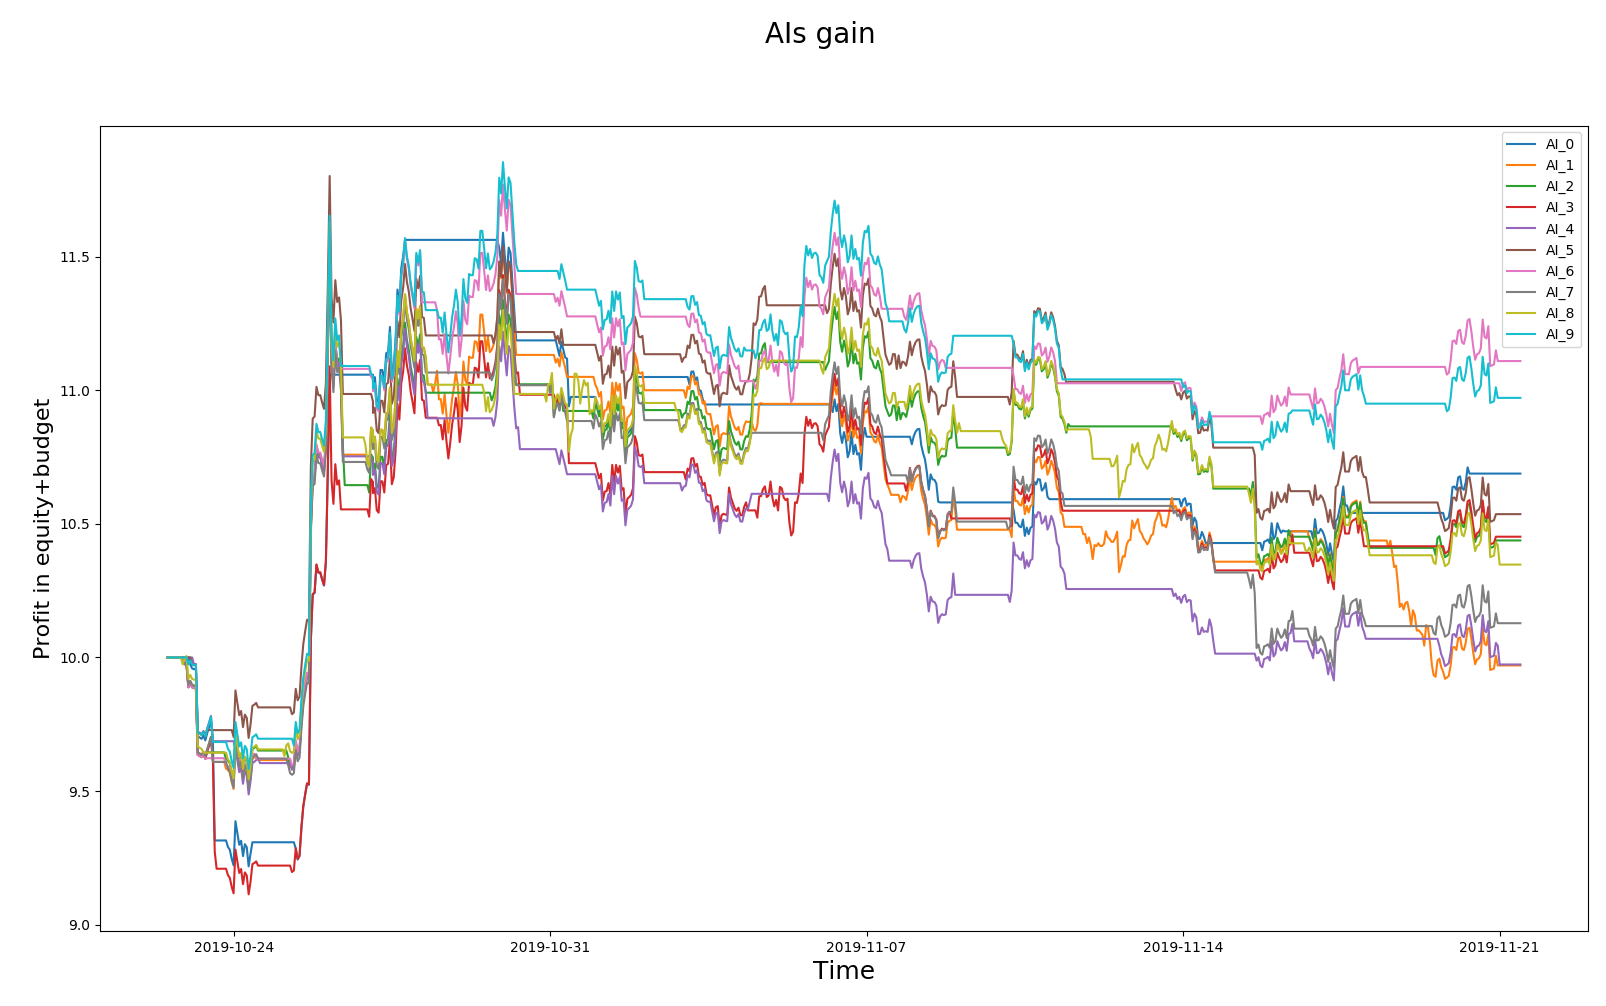
\includegraphics[width=\linewidth]{ai_gains}%TODO: no AI-GAINs ma ai_performance!
	\end{center}
	\caption{Figura: grafico comparativo dei risultati prodotti da 10 differenti AI di Sentyment. In questo caso è analizzata la funzione \textit{performance} (Formula 6) per ciascuna delle AI prese in considerazione. La funzione è calcolata partendo dall'inizio del dataset (BITCOIN-EURO a partire da inizio 2014, fino a inizio 2020) e aggiungendo continuamente step di 200 candele orarie. Il risultato è quindi la performance cumulativa. Alcune AI si posizionano sempre in alto rispetto ad altre ed è per questo motivo che è necessario sceglierne una migliore fra tutte. Le migliori si sorpassano spesso lungo il tempo e infatti andrebbero scambiate a periodi di tempo da stabilire.}
\end{fig}
\section{Test comparativi e Meta-learner}
%https://tams.informatik.uni-hamburg.de/publications/2019/MSc_Ronja_Gueldenring.pdf
Verrà ora affrontato il tema centrale della tesi: sviluppare una AI supervisore in grado di scegliere un rappresentante migliore fra una serie di agenti intelligenti.\\
Sentyment è composta da numerose AI che creano strategie di investimento e ognuna opera indipendentemente dalle altre, producendo costantemente dati relativi ai nuovi trade aggiornati in tempo reale e differenziandosi leggermente dalle altre. Le AI attive sono solitamente 12, ma il numero potrebbe variare a seconda degli iperparametri scelti durante il ciclo di test. Per ogni AI sono noti i suoi \textit{trigger}, cioè le operazioni di buy / sell relative ad un certo istante di tempo che l'agente ha prodotto.

\begin{fig}
    \begin{center}
    	\begin{tabular}{||c c ||} 
    		\hline
    		time & trigger \\ [0.5ex] 
    		\hline\hline
    		2020-01-13 18:00:00 & 1 \\
    		\hline
    		2020-01-13 19:00:00 & 0 \\
    		\hline
    		2020-01-13 20:00:00 & 0 \\
    		\hline
    		2020-01-13 21:00:00 & 0 \\
    		\hline
    		2020-01-13 22:00:00 & 0 \\
    		\hline
    		2020-01-13 23:00:00 & -1 \\ [1ex] 
    		\hline
    	\end{tabular}
    \end{center}
	\caption{Tabella: elenco di record che rappresentano il risultato prodotto da una delle AI di Sentyment. Sono state considerate le candele orarie: per ogni ora si ha il segnale di buy / sell / hold. I trigger sono rappresentati da un valore numerico: 0 per hold, 1 per buy e -1 sell. In questa tabella è stata aperta una posizione di acquisto il 13 gennaio 2020 alle ore 18:00 ed è stato venduto il titolo alle 23:00}
\end{fig}
\begin{fig}
	\begin{center}
		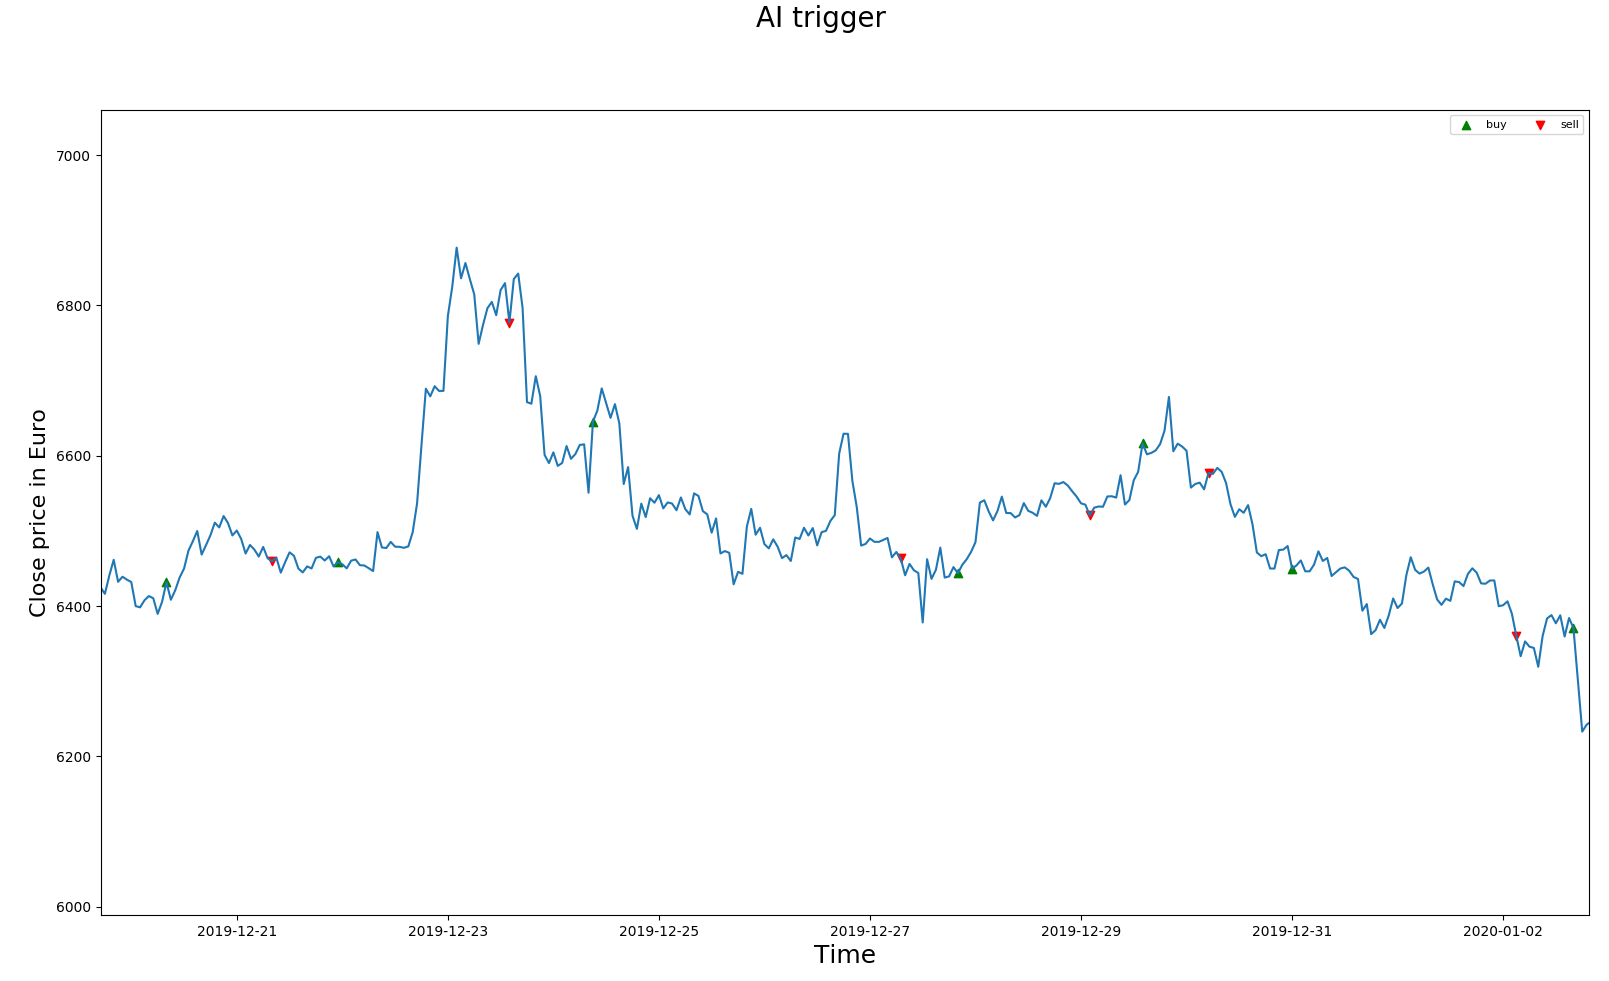
\includegraphics[width=\linewidth]{ai_trigger}
	\end{center}
	\caption{Figura: Esempio di grafico dei prezzi di chiusura di BITCOIN-EURO in un certo periodo, e i \textit{trigger} di una AI di Sentyment. Si nota che i segnali buy / sell non corrispondono esattamente fra una AI e l'altra, confrontando questo grafico con la prossima immagine, ma sono leggermente spostati. Ognuna produce strategie differenti e, anche se probabilmente molte AI identificano gli stessi trend nel grafico, alcune potrebbero decidere di comprare o vendere leggermente prima, o dopo, rispetto alle altre.}
\end{fig}
\begin{fig}
	\begin{center}
		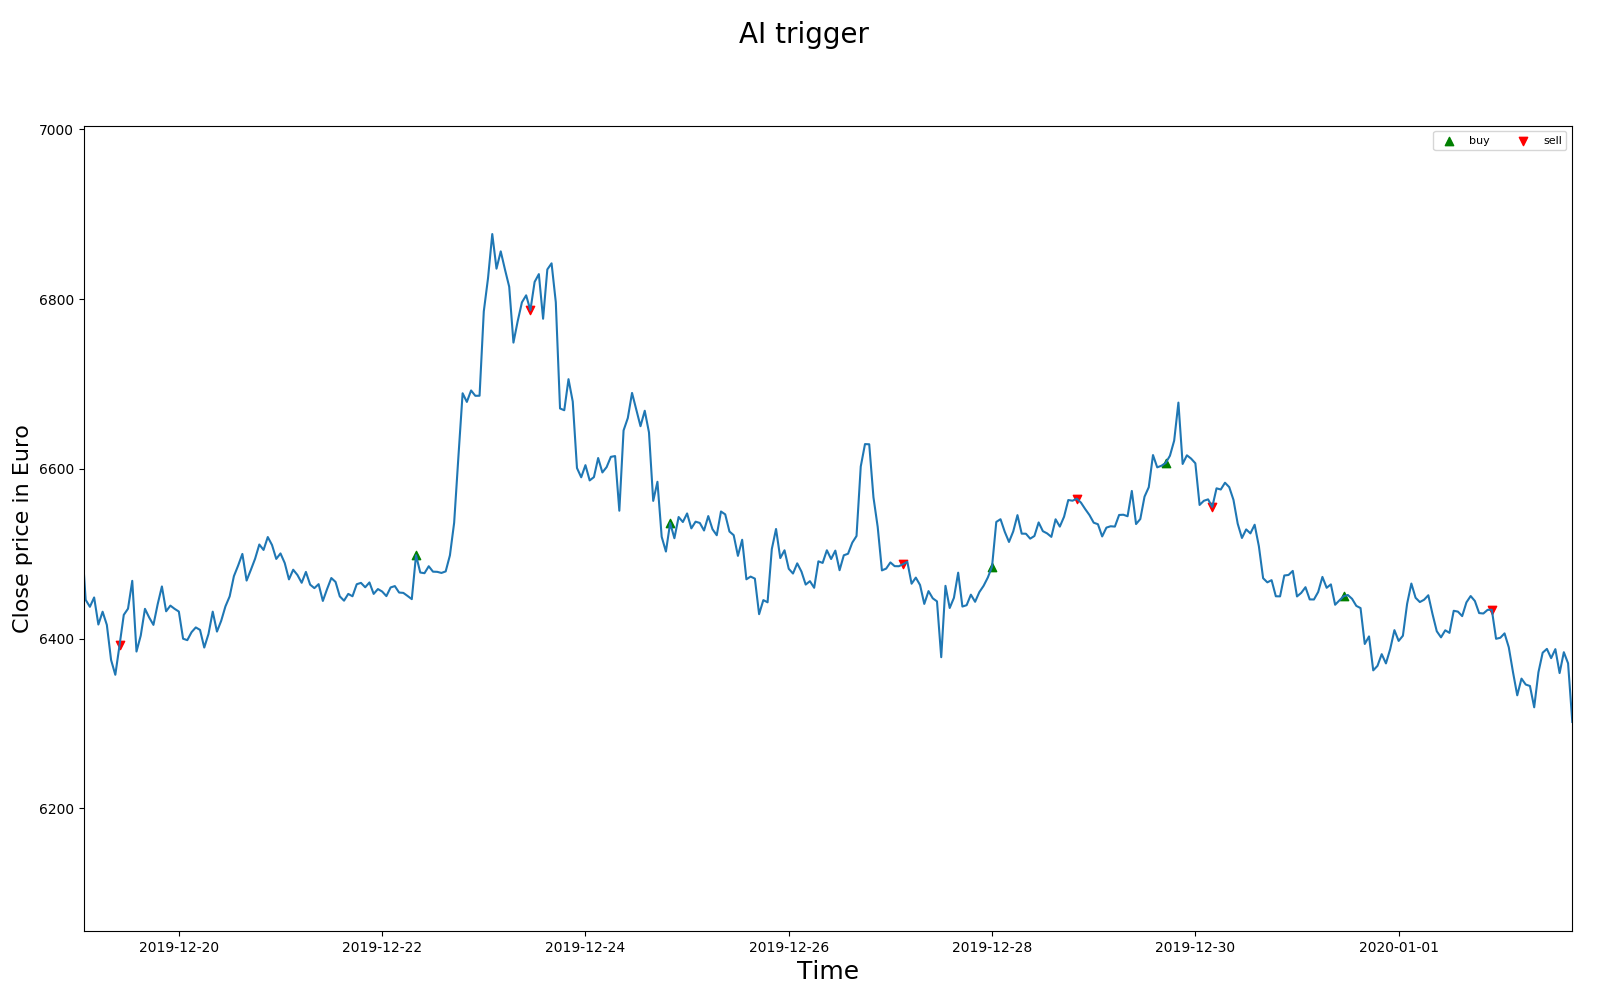
\includegraphics[width=\linewidth]{ai_trigger2}
	\end{center}
	\caption{Figura: Secondo grafico dei prezzi di chiusura per lo stesso ticker e periodo temporale del precedente. È considerata una differente AI questa volta, e i segnali buy / sell sono leggermente diversi.}
\end{fig}
\\~\\
Inizialmente si può supporre di raccogliere dati per alcune settimane e poi utilizzare questo dataset per scegliere una AI, quindi ricominciare la fase di osservazione, in cui si raccolgono dati per alcune settimane, e ripetere il ciclo; in una fase più avanzata, però, anche il tempo lungo cui prendere le misure diventa un parametro del supervisore e deve essere deciso.
Unendo l'elenco di operazioni di ogni AI per un certo periodo con il dataset OHLCV dei prezzi (Tabella 2), è possibile calcolare uno \textit{score} basato su numerose statistiche, descritto nella precedente sezione. La AI supervisore, fondandosi su questo score, sceglie qual è la AI che lo massimizza di più rispetto alle altre, tenendo conto anche del fatto che il punteggio varia a seconda del periodo di tempo considerato e anche all'interno dello stesso dataset, se si scelgono punti iniziali e finali differenti.\\
\begin{fig}
	\begin{center}
	\begin{tabular}{||c c c c c ||} 
		\hline
		time & price & trigger\_AI\_1 & trigger\_AI\_2 & trigger\_AI\_3 \\ [0.5ex] 
		\hline\hline
		2020-01-13 18:00:00 & 153.3 & 1 & 1 & 0\\
		\hline
		2020-01-13 19:00:00 & 153.3 & 0 & 0 & 0\\
		\hline
		2020-01-13 20:00:00 & 152.9 & 0 & 0 & 1\\
		\hline
		2020-01-13 21:00:00 & 153.5 & 0 & 0 & -1\\
		\hline
		2020-01-13 22:00:00 & 153.5 & 0 & -1 & 0\\
		\hline
		2020-01-13 23:00:00 & 153.7 & -1 & 0 & 0\\ [1ex] 
		\hline
	\end{tabular}
	\end{center}
	\caption{Tabella: elenco di record contenenti le scelte di alcune AI, unito ai prezzi di chiusura delle candele associate. Questi dataset sono tutto ciò che il supervisore necessita in input per essere allenato e operare la sua scelta.}
\end{fig}
\\~\\Un approccio di machine learning che si adatta particolarmente al contesto descritto è il \textit{reinforcement learning}, tecnica di apprendimento automatico che punta a realizzare agenti autonomi in grado di scegliere azioni da compiere per il conseguimento di determinati obiettivi tramite interazione con l'ambiente in cui sono immersi.
L'apprendimento per rinforzo \cite{rl} è uno dei tre paradigmi principali dell'apprendimento automatico, insieme a \textit{supervised} e \textit{unsupervised learning}\footnote{L'apprendimento supervisionato (supervised learning) è una tecnica di apprendimento automatico che mira a istruire un sistema in modo da consentirgli di elaborare automaticamente previsioni sui valori di uscita di un sistema rispetto ad un input sulla base di una serie di esempi ideali, costituiti da coppie di input e di output, che gli vengono inizialmente forniti.\\ L'apprendimento non supervisionato (unsupervised) consiste nel fornire al sistema una serie di input (esperienza del sistema) che egli riclassificherà ed organizzerà sulla base di caratteristiche comuni per cercare di effettuare ragionamenti e previsioni sugli input successivi. Al contrario dell'apprendimento supervisionato, durante l'apprendimento vengono forniti all'apprendista solo esempi non annotati, in quanto le classi non sono note a priori ma devono essere apprese automaticamente. }. A differenza degli altri due, questo paradigma si occupa di problemi di decisioni sequenziali, in cui l'azione da compiere dipende dallo stato attuale del sistema e ne determina quello futuro.\\
La qualità di un'azione è data da un valore numerico di "ricompensa", ispirata al concetto di reinforcement, che ha lo scopo di incoraggiare comportamenti corretti dell'agente. Questo tipo di apprendimento è solitamente modellato tramite i processi decisionali di Markov\footnote{Un processo decisionale di Markov (MDP, Markov Decision Process) è un estensione di Markov Chain e fornisce un framework matematico per la modellazione di processi decisionali. Si basa sull'assunto che la decisione futura dipende soltanto dalle condizioni presenti e non da quelle passate. È alla base di molti algoritmi di reinforced learning} e può essere effettuato con diverse tipologie di algoritmi.\\~\\
Questa tecnica si basa sul presupposto che all'interno di un sistema si possano: scegliere degli output sulla base degli input ricevuti, valutare l'efficacia degli output rispetto ad un preciso parametro di riferimento e cambiare il meccanismo di scelta degli input per massimizzare la valutazione di efficacia.\\
Quando si effettua una scelta efficace allora la valutazione di efficacia manda in output un premio proporzionale all'efficacia della scelta. Quando invece è effettuata una scelta inefficace allora l'output della valutazione manda una penalità proporzionale. Osservando le scelte e le ricompense, si cerca di modificare la funzione matematica che regola le scelte in modo da massimizzare la quantità e la qualità dei "premi".\\

\begin{fig}
	\begin{center}
			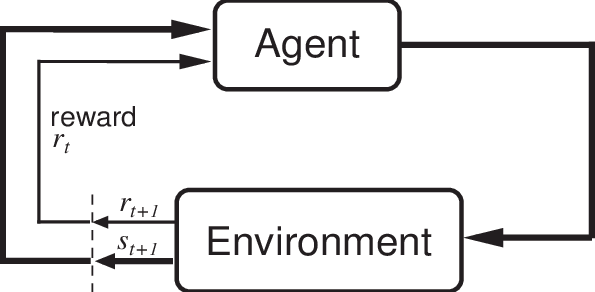
\includegraphics[width=10cm]{rl}
	\end{center}
	\caption{Figura: Idea generale di \textit{reinforcement learning}: un agente interagisce con l'ambiente per imparare dall'esperienza. Per ogni istante di tempo \textit{t} l'agente è in un certo stato \textit{S\textsubscript{t}} ed esegue l'azione \textit{A\textsubscript{t}}. Come risultato, passa in un nuovo stato \textit{S\textsubscript{t+1}} e riceve una ricompensa \textit{R\textsubscript{t+1}}}
\end{fig}

\\~\\Nel contesto di Sentyment il supervisore rappresenta l'agente che opera le scelte. L'ambiente (i dati in input) sono i dataset di qualche settimana che, a ogni iterazione del ciclo di scelta della nuova AI rappresentante, sono forniti all'algoritmo di reinforcement learning. La scelta che il supervisore deve operare ad ogni passo è decidere quale fra le dodici AI sta, secondo lui, agendo meglio delle altre; mentre l'output della scelta, ovvero la valutazione di efficacia, è il risultato di una funzione di score calcolata con indicatori statistici finanziari a partire dai trigger della AI scelta, il cui risultato viene confrontato con quello prodotto dalle altre AI competitori.\\~\\Ritorna ancora una volta il concetto di \textit{score}, o \textit{metrica}. La metrica (formula (6)) guida l'agente supervisore nelle sue scelte: verrà ricompensato positivamente se, ad ogni iterazione, sceglie la AI fra le 12 che produce lo score massimo fra tutte le altre, mentre la scelta si considera negativa se non si verifica questa condizione.

\subsection{Multi-armed bandit e Meta-learner}
Una soluzione nota che si adatta alla situazione e fa uso di tecniche di reinforcement learning, implementata usando diversi algoritmi. La versione classica di \textit{multi-armed bandit} discosta leggermente da questo ambito ma può essere revisionato per trarre vantaggio dalla sua semplicità.\cite{rl}\\ Nella teoria delle probabilità, multi-armed bandit è un problema in cui un insieme fisso limitato di risorse deve essere allocato tra scelte concorrenti (alternative) in un modo che massimizza il guadagno atteso, quando le proprietà di ciascuna scelta sono conosciute solo parzialmente al momento dell'allocazione e possono essere meglio comprese col passare del tempo o allocando risorse per la scelta. Questo è un classico problema di apprendimento per rinforzo che esplicita il dilemma del compromesso tra esplorazione (\textit{exploration}) e sfruttamento (\textit{exploitation}).\\ Il nome deriva dall'immaginare un giocatore d'azzardo in una fila di slot machine, che deve decidere su quali macchine giocare, quante volte giocare ogni macchina e in quale ordine giocarle, e se continuare con la macchina corrente o provarne un'altra. Nel problema, ogni macchina fornisce una ricompensa casuale da una distribuzione di probabilità specifica per quella macchina. L'obiettivo del giocatore è massimizzare la somma dei premi guadagnati attraverso una sequenza di tiri della leva. Il compromesso cruciale che il giocatore deve affrontare ad ogni prova è tra "sfruttamento" della macchina che ha il più alto profitto atteso e "esplorazione" per ottenere maggiori informazioni sui guadagni previsti delle altre macchine.


%TODO: epsilon greedy e funzione Q(...) di apprendimento! https://lilianweng.github.io/lil-log/2018/01/23/the-multi-armed-bandit-problem-and-its-solutions.html
\begin{fig}
	\begin{center}
		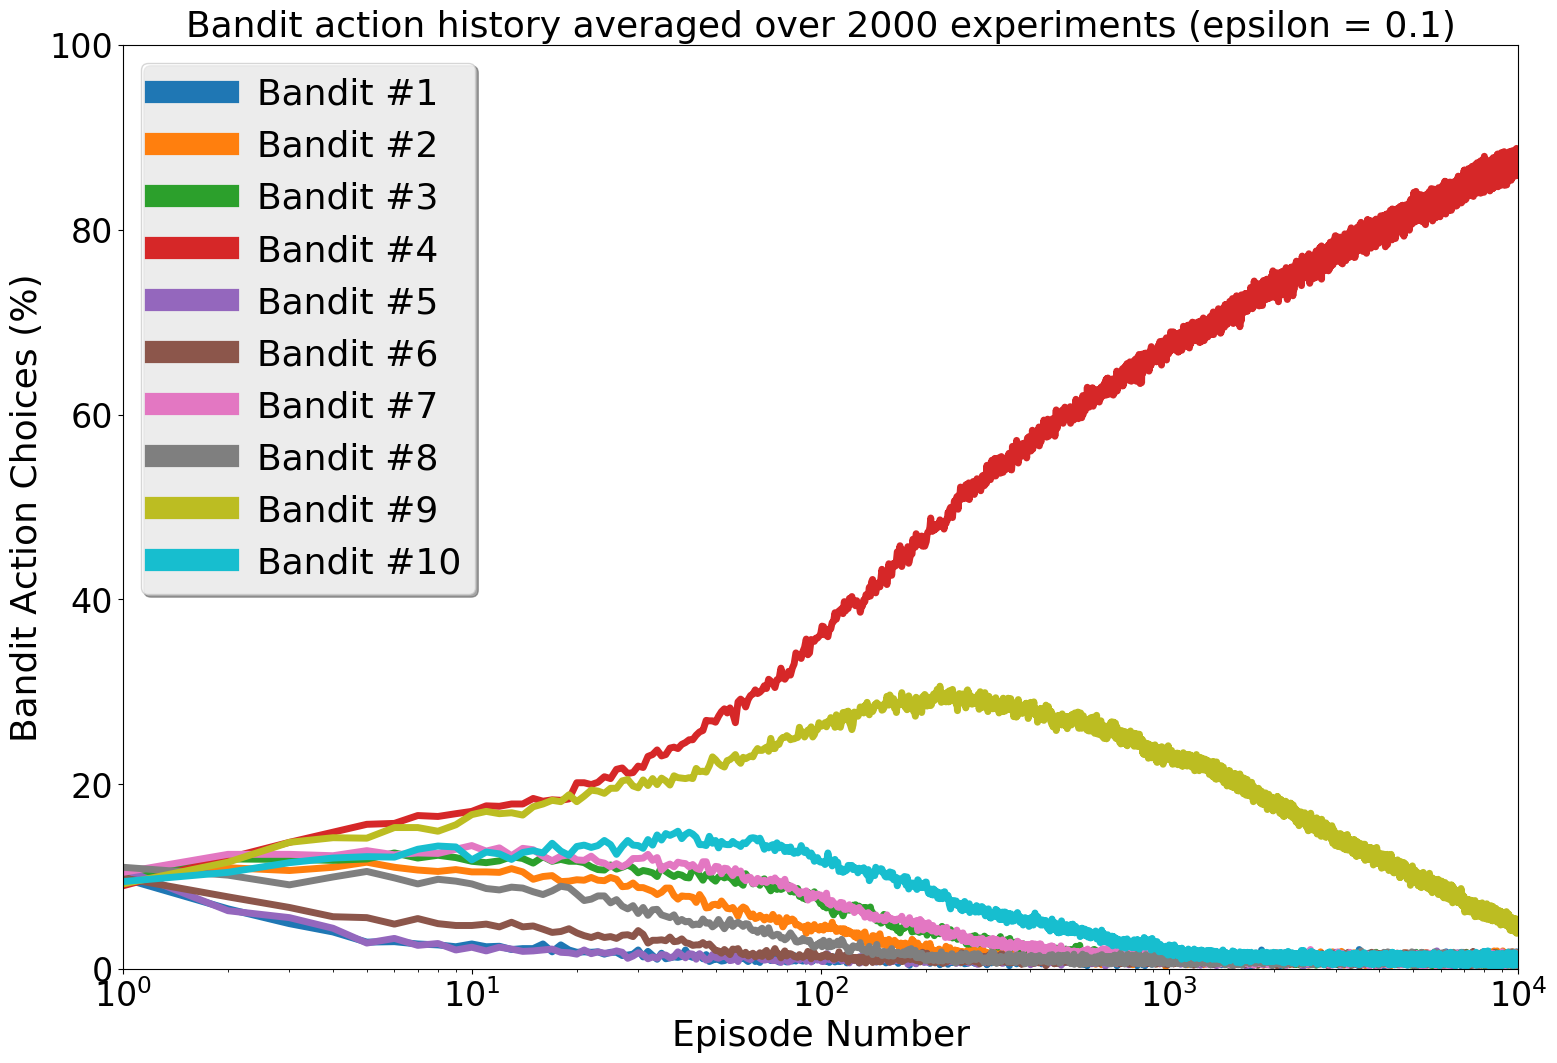
\includegraphics[width=\linewidth]{bandit1}
	\end{center}
	\caption{\\~\\Figura: Esempio di scelte effettuate durante il training di un agente multi-armed bandit. Al crescere del numero di scelte effettuate (Episode number), si avrà una concentrazione sempre maggiore della scelta su uno specifico bandit, quello che, secondo l'algoritmo, è il più promettente. In questo caso si può notare come il bandit preferito sia il numero 4. Già dopo 10\textsuperscript{2} scelte, i competitori si riducono praticamente a due soltanto, il bandit 4 e il 9. Poco dopo, però, è il numero 4 ad essere scelto sempre più spesso nella fase di training.}
\end{fig}
\\~\\La versione adattata prevede di scegliere un dataset di prezzi e trigger delle AI e suddividerlo in un numero di \textit{step}. Per ogni step, è calcolato lo \textit{score} di ciascuna delle AI in gioco. L'agente effettua la sua scelta valutando fra esplorare nuove soluzioni, con possibilità di trovare un nuovo migliore, oppure scegliere di nuovo la AI che si è mostrata migliore nelle precedenti iterazioni. Questa scelta è guidata dal \textit{tasso di apprendimento} (\textit{epsilon}), un parametro che determina il comportamento dell'agente variando da 0 a 1, dove 0 rappresenta il non-apprendimento, la scelta si protrae sempre uguale, mentre 1 farebbe sì che l'agente si interessi solo delle informazioni recenti.\\ A seconda della scelta effettuata, cioè puntare sul vecchio migliore o esplorare un nuovo concorrente, l'agente riceve una \textit{ricompensa}. L'implementazione dell'algoritmo multi-armed bandit prevede soltanto una ricompensa positiva (1, il bandit scelto vince questo giro) o negativa (0, il bandit non è vincente); la ricompensa positiva si ha quando l'agente, in questo step, ha scelto l'AI che ha prodotto lo score più alto rispetto a tutte le altre. Viceversa, la ricompensa sarà negativa.\\ Continuando nelle scelte attraverso i vari step, fino alla fine del dataset, l'agente aggiorna la sua funzione che regola le scelte e, dopo un sufficiente numero di iterazioni e ripetendo anche più volte lo stesso esperimento, l'algoritmo è in grado di scegliere con precisione sempre più alta la AI migliore.\\~\\ Alla fine di questa fase di training, l'agente fornisce l'elenco dello storico delle scelte effettuate. La AI migliore è quella scelta il maggior numero di volte rispetto a tutte le altre.

\subsection{Scelta dei parametri}
L'algoritmo multi-armed bandit originale definisce già una serie di parametri che possono modificare l'esito delle scelte e dovrebbero essere decisi analizzando il contesto e scegliendo i migliori a seconda della situazione. In aggiunta, l'adattamento della soluzione al dominio di Sentyment costringe a prendere alcune decisioni.\\~\\ Il problema delle slot machine prevede come step la scelta di un bandit e la successiva ricompensa immediata: tirando la leva si vince o si perde. Poi si ripete l'esperimento un gran numero di volte. Nel caso di Sentyment, è evidente che questa situazione non si può modellare così facilmente, non esiste vincita o perdita immediata. È stato pensato un adattamento in cui si divide il dataset di training in step da non meno di 25 candele, si calcola lo score che ogni AI produce considerando quei 25 record e si sceglie la migliore all'interno di questo frame. Poi l'agente effettua la sua scelta e ottiene la ricompensa di conseguenza (l'agente non conosce gli score). Si procede considerando i prossimi 25 record e si ripete fino alla fine del dataset.\\ Procedendo con step di 25 candele, che ne caso di candele orarie si tratta di circa un giorno di dati, si dà la possibilità alle AI di effettuare abbastanza operazioni di acquisto e vendita in modo da avere una quantità sufficiente di dati per poter calcolare lo score, dato che i trigger delle AI sono molto sparsi (pochi buy / sell). Si simula dunque una situazione in cui le AI sono valutate circa su una base giornaliera.\\~\\ A causa della gran quantità di dati necessari per un singolo step, scelta dovuta in seguito alla proprietà intrinseche delle AI e del contesto finanziario, sono di conseguenza necessarie moltissime candele per allenare l'algoritmo di reinforcement learning. L'agente deve compiere come minimo 500 step per il training, con esempi di anche 2000 step \cite{46}, quindi significa che servono almeno 25*500 candele, per un totale di 12500 candele, cioè 520 giorni. 


\textcolor{red}{Tutto ciò non è vero, non hai ancora provato. Come fai a fare in modo che su 2 anni di dati cambi qualcosa allungare di 2 settimane? Allora le AI vanno cambiate dopo molto più di 2 settimane! OPPURE non devi considerare veramente tutte ste candele, ma riesci a farlo in sole 2 settimane oppure, un mese. 
QUINDI: - consideri dataset di 1 anno per scelta + scegli migliore; dopo 2 settimane consideri 1 anno + 2 settimane + scegli migliore OPPURE
		- consideri dataset di 2 settimane (1 mese) + scegli migliore; ti sposti avanti di 2 settimane (1 mese) + scegli datset di 2 settimane (1 mese) + scegli migliore ?
	
	MA PROPRIO RILEGGI TUTTA STA SEZIONE UNA VOLTA FATTI I TEST.}

%TODO: esempio introduttivo con grafici XETH e XBT ma poi spiega che non è richiesto / non serve fare tante monete ma di concentrarsi su una moneta sola (XXBT) e poi parti con XBT. Grafici ai trigger esempio (2) con relativo price, e poi PRICE + GAIN dataset piccolo e poi PRICE + GAIN + PERFORMANCE dataset grosso e poi SCELTA AI META-LEARNER.

Infine tutto il training sull'intero dataset, detto \textit{experiment}, va ripetuto per molte volte, per completare il training. Il numero deve essere abbastanza alto e quindi è stato scelto, in accordo con altri esempi, 10000.\\~\\ Non ci sono altri parametri da considerare per l'algoritmo di multi-armed bandit, oltre al numero di step e la lunghezza del dataset. La funzione di ricompensa è già stata descritta, e anche \textit{epsilon}, che determina il tasso di apprendimento. Se gli altri parametri sono stati ricavati o imposti dall'adattamento del problema al contesto di Sentyment, quest'ultimo è una proprietà del metodo di apprendimento e non cambia. È stato scelto fisso al 10\%. %TODO: cosa significa sto parametro?

%TODO: parlare di dati reali ottenuti, coi grafici simili a quelli sopra ma nel tuo caso
\section{Test framework workflow}
(Qua oppure nuova subsectin su? cambio nome? test workflow comunque ci vuole) Ora si analizzeranno i risultati ottenuti applicando l'algoritmo di multi-armed bandit al contesto descritto. È considerato un dataset di prezzi che parte da .. .a ... contenente circa ... record. Sono scelte alcune fra le possibili AI a disposizione, a formare un pool di 12 competitori e lo score utilizzato è quello della formula (6). Il dataset è diviso in ... step, in modo da dare all'agente la possibilità di fare diverse prove

\section{Test assoluti: maximum profit e genetic AI}
%TODO: come in "test per sentyment" ma nel dettaglio
quanto guadagno produce la AI rispetto al \textit{massimo guadagno} assoluto che si sarebbe potuto ottenere sfruttando al massimo gli investimenti.\\ L'idea deriva dalle tecniche di test per Decision Support AI. Il testing di questa tipologia di AI è condotto attraverso il confronto delle decisioni prese dalla AI rispetto ad un \textit{golden standard}, un modello di riferimento che rappresenta la migliore situazione possibile e il massimo risultato che un algoritmo possa mai ottenere.

\newpage
\chapter{Conclusioni e lavori futuri}
\label{cap5}
Aggiungere un ulteriore livello di learning sopra il meta-learner, che apprende dal supervisore qual è l'intervallo di tempo migliore in cui cambiare AI scelta.

\newpage

%
%			BIBLIOGRAFIA
%
\begin{thebibliography}{9}
	\bibitem{nn1}
	Lawrence, R. (1997). Using neural networks to forecast stock market prices. University of Manitoba, 333, 2006-2013.
	\bibitem{whitenn}
	White, H. (1988). Economic prediction using neural networks: The case of IBM daily stock returns.
	\bibitem{puann}
	Phua, P. K. H., Ming, D., \& Lin, W. (2000, July). Neural network with genetic algorithms for stocks prediction. In Fifth Conference of the Association of Asian-Pacific Operations Research Societies, 5th-7th July, Singapore. sn.
	\bibitem{kimnn}
	Kim, K. J., \& Han, I. (2000). Genetic algorithms approach to feature discretization in artificial neural networks for the prediction of stock price index. Expert systems with Applications, 19(2), 125-132.
	\bibitem{nng}
	Garliauskas, A. (1999, October). Neural network chaos and computational algorithms of forecast in finance. In IEEE SMC'99 Conference Proceedings. 1999 IEEE International Conference on Systems, Man, and Cybernetics (Cat. No. 99CH37028) (Vol. 2, pp. 638-643). IEEE.
	\bibitem{nns}
	Schumann, M., \& Lohrbach, T. (1993, January). Comparing artificial neural networks with statistical methods within the field of stock market prediction. In [1993] Proceedings of the Twenty-sixth Hawaii International Conference on System Sciences (Vol. 4, pp. 597-606). IEEE.
	\bibitem{nny}
	Yoon, Y., Swales Jr, G., \& Margavio, T. M. (1993). A comparison of discriminant analysis versus artificial neural networks. Journal of the Operational Research Society, 44(1), 51-60.
	\bibitem{nnk}
	Kim, J. W., Weistroffer, H. R., \& Redmond, R. T. (1993). Expert systems for bond rating: a comparative analysis of statistical, rule‐based and neural network systems. Expert systems, 10(3), 167-172.
	\bibitem{nnp}
	Patuwo, E., Hu, M. Y., \& Hung, M. S. (1993). Two‐group classification using neural networks. Decision Sciences, 24(4), 825-845.
	\bibitem{nns2}
	Subramanian, V., Hung, M. S., \& Hu, M. Y. (1993). An experimental evaluation of neural networks for classification. Computers \& operations research, 20(7), 769-782.
	\bibitem{es}
	Chalup, S., \& Maire, F. (1999, July). A study on hill climbing algorithms for neural network training. In Proceedings of the 1999 Congress on Evolutionary Computation-CEC99 (Cat. No. 99TH8406) (Vol. 3, pp. 2014-2021). IEEE.
	\bibitem{know-nn}
	Hong, T., \& Han, I. (2002). Knowledge-based data mining of news information on the Internet using cognitive maps and neural networks. Expert systems with applications, 23(1), 1-8.
	\bibitem{news-nn}
	Fung, G. P. C., Yu, J. X., \& Lam, W. (2002, May). News sensitive stock trend prediction. In Pacific-Asia Conference on Knowledge Discovery and Data Mining (pp. 481-493). Springer, Berlin, Heidelberg.
	\bibitem{know-nn2}
	Kohara, K., Ishikawa, T., Fukuhara, Y., \& Nakamura, Y. (1997). Stock price prediction using prior knowledge and neural networks. Intelligent Systems in Accounting, Finance \& Management, 6(1), 11-22.
	\bibitem{news-nn2}
	Fung, G. P. C., Yu, J. X., \& Lam, W. (2003, March). Stock prediction: Integrating text mining approach using real-time news. In 2003 IEEE International Conference on Computational Intelligence for Financial Engineering, 2003. Proceedings. (pp. 395-402). IEEE.
	\bibitem{fuzzy-nn1}
	Kuo, R. J., Chen, C. H., \& Hwang, Y. C. (2001). An intelligent stock trading decision support system through integration of genetic algorithm based fuzzy neural network and artificial neural network. Fuzzy sets and systems, 118(1), 21-45.
	\bibitem{fuzzy-nn2}
	Kuo, R. J., Lee, L. C., \& Lee, C. F. (1996, October). Integration of artificial neural networks and fuzzy delphi for stock market forecasting. In 1996 IEEE International Conference on Systems, Man and Cybernetics. Information Intelligence and Systems (Cat. No. 96CH35929) (Vol. 2, pp. 1073-1078). IEEE.
	\bibitem{emh1}
	Lowe, D., \& Webb, A. R. (1991, February). Time series prediction by adaptive networks: A dynamical systems perspective. In IEE Proceedings F (Radar and Signal Processing) (Vol. 138, No. 1, pp. 17-24). IET Digital Library.
	\bibitem{emh2}
	Maddala, G. S., \& Lahiri, K. (1992). Introduction to econometrics (Vol. 2). New York: Macmillan.
	\bibitem{emh3}
	HellStrom, T., \& Holmstrom, K. (1998). Predicting the stock market. Unpublished Thesis, Malardalen University, Department of Mathematics and Physics, Vasteras, Sweden.
	\bibitem{emh4}
	Malkiel, B. G., \& Fama, E. F. (1970). Efficient capital markets: A review of theory and empirical work. The journal of Finance, 25(2), 383-417.
	\bibitem{emh0}
	Tsibouris, G., \& Zeidenberg, M. (1995). Testing the efficient markets hypothesis with gradient descent algorithms. In Neural networks in the capital markets (Vol. 8, pp. 127-136). Chichester, UK: Wiley.
	\bibitem{nn-eyden}
	Van Eyden, R. J. (1996). The Application of Neural Networks in the Forecasting of Share Prices (Finance and Technology Publishing, Haymarket, VA).
	\bibitem{23}
	Lawrence, R. (1997). Using neural networks to forecast stock market prices. University of Manitoba, 333, 2006-2013.
	\bibitem{34}
	Van Eyden, R. J. (1996). The Application of Neural Networks in the Forecasting of Share Prices (Finance and Technology Publishing, Haymarket, VA).
	\bibitem{33}
	Refenes, A. P., Zapranis, A. D., \& Francis, G. (1995). Modeling stock returns in the framework of APT: a comparative study with regression models. In Neural networks in the capital markets (Vol. 7, pp. 101-126). John Wiley \& Sons Chichester.
	\bibitem{36}
	Steiner, M. (1995). Neural networks as an alternative stock market model.
	\bibitem{2}
	Dash, M., \& Liu, H. (1997). Feature selection for classification. Intelligent data analysis, 1(3), 131-156.
	\bibitem{11}
	Hiemstra, Y. (1995). Modeling structured nonlinear knowledge to predict stock market returns. Chaos \& Nonlinear Dynamics in the Financial Markets: Theory, Evidence and Applications, Irwin, Chicago, IL, 163-175.
	\bibitem{41}
	Tsaih, R., Hsu, Y., \& Lai, C. C. (1998). Forecasting S\&P 500 stock index futures with a hybrid AI system. Decision Support Systems, 23(2), 161-174.
	\bibitem{44}
	Vapnik, V. N. (1999). An overview of statistical learning theory. IEEE transactions on neural networks, 10(5), 988-999.
	\bibitem{46}
	Yang, H., Chan, L., \& King, I. (2002, August). Support vector machine regression for volatile stock market prediction. In International Conference on Intelligent Data Engineering and Automated Learning (pp. 391-396). Springer, Berlin, Heidelberg.
	\bibitem{43}
	Vapnik, V. N. (1999). An overview of statistical learning theory. IEEE transactions on neural networks, 10(5), 988-999.
	\bibitem{15}
	Kim, K. J. (2003). Financial time series forecasting using support vector machines. Neurocomputing, 55(1-2), 307-319.
	\bibitem{38}
	Tay, F. E., \& Cao, L. (2001). Application of support vector machines in financial time series forecasting. omega, 29(4), 309-317.
	\bibitem{39}
	Tay, F. E. H., \& Cao, L. J. (2001). A comparative study of saliency analysis and genetic algorithm for feature selection in support vector machines. Intelligent Data Analysis, 5(3), 191-209.
	\bibitem{40}
	Trippi, R. R., \& Turban, E. (1992). Neural networks in finance and investing: Using artificial intelligence to improve real world performance. McGraw-Hill, Inc..
	\bibitem{17}
	Kim, K. J. (2004). Toward global optimization of case-based reasoning systems for financial forecasting. Applied intelligence, 21(3), 239-249.
	\bibitem{29}
	Ng, A., \& Fu, A. W. C. (2003, April). Mining frequent episodes for relating financial events and stock trends. In Pacific-Asia Conference on Knowledge Discovery and Data Mining (pp. 27-39). Springer, Berlin, Heidelberg.
	\bibitem{26}
	Maheu, J. M., \& McCurdy, T. H. (2004). News arrival, jump dynamics, and volatility components for individual stock returns. The Journal of Finance, 59(2), 755-793.
	\bibitem{4}
	Fawcett, T., \& Provost, F. J. (1996, August). Combining Data Mining and Machine Learning for Effective User Profiling. In KDD (pp. 8-13).
	\bibitem{13}
	Hong, T., \& Han, I. (2004). Integrated approach of cognitive maps and neural networks using qualitative information on the World Wide Web: the KBNMiner. Expert Systems, 21(5), 243-252.
	%\bibitem{}
	%Bengio, Y. (2009). Learning deep architectures for AI. Foundations and trends® in %Machine Learning, 2(1), 1-127.
	%\bibitem{}
	%An, G. (1996). The effects of adding noise during backpropagation training on a %generalization performance. Neural computation, 8(3), 643-674.
	\bibitem{aitest}
	Schmelzer, R. (2020, January 3). How Do You Test AI Systems?. Forbes. Last accessed 21th Feb 2020:
	https://www.forbes.com/sites/cognitiveworld/2020/01/03/how-do-you-test-ai-systems.
	\bibitem{46} 
	Wong, A. (2017, September 25). Solving the Multi-Armed Bandit Problem. Last accessed 21th Feb 2020:
	https://towardsdatascience.com/solving-the-multi-armed-bandit-problem-b72de40db97c
	\bibitem{rl}
	Sutton, R. S., \& Barto, A. G. (1998). Introduction to reinforcement learning (Vol. 135). Cambridge: MIT press.
	\bibitem{}
	Guijarro-Berdiñas, B., \& Alonso-Betanzos, A. (2002). Empirical evaluation of a hybrid intelligent monitoring system using different measures of effectiveness. Artificial Intelligence in Medicine, 24(1), 71-96.
\end{thebibliography}
\end{document}


 
